%======================================================
% Technische Universitaet Darmstadt
% Fachbereich Elektrotechnik und Inmatlformationstechnik
% Control Theory and Robotics Lab
% Prof. Dr.-Ing. J. Adamy
%======================================================
% Vorlage fuer Abschlussarbeiten
% Stand: 12.2012
% Wichtig: Kompilieren mit PDFLaTeX wird empfohlen
% Offizielle TUD-LaTeX-Vorlage erhaeltlich unter:
% http://exp1.fkp.physik.tu-darmstadt.de/tuddesign/
%======================================================
\documentclass[twoside,bigchapter,colorback,accentcolor=tud4b,11pt]{tudreport}
%======================================================
% colorback = Bereich unter Titel mit Hintergrundfarbe
% colorbacktitle = Titel mit Hintergrundfarbe (Akzent)
% RTR-Bl2au = accentcolor=tud1b		
% Grau = accentcolor=tud0a 
% blackrule fuer schwarze Leiste
% nochapterpage = do not start chapters on new page
% oneside = print only on one side of the page
%======================================================

%======================================================
% General package loading and definitions
%======================================================
\usepackage{color}
\usepackage{listings}
\usepackage{caption}

\newcounter{nalg}[chapter] % defines algorithm counter for chapter-level
\renewcommand{\thenalg}{\thechapter .\arabic{nalg}} %defines appearance of the algorithm counter
\DeclareCaptionLabelFormat{algocaption}{Algorithm \thenalg} % defines a new caption label as Algorithm x.y

\lstnewenvironment{algorithmHu}[1][] %defines the algorithm listing environment
{   
    \refstepcounter{nalg} %increments algorithm number
    \captionsetup{labelformat=algocaption,labelsep=colon} %defines the caption setup for: it ises label format as the declared caption label above and makes label and caption text to be separated by a ':'
    \lstset{ %this is the stype
        mathescape=true,
        frame=tB,
        numbers=left, 
        numberstyle=\tiny,
        basicstyle=\scriptsize, 
        keywordstyle=\color{black}\bfseries\em,
        keywords={,input, output, return, datatype, function, in, if, else, foreach, while, begin, end, } %add the keywords you want, or load a language as Rubens explains in his comment above.
        numbers=left,
        xleftmargin=.04\textwidth,
        #1 % this is to add specific settings to an usage of this environment (for instnce, the caption and referable label)
    }
}
{}
 
 
\usepackage{pythonhighlight}
\usepackage{lingmacros}
\usepackage{tree-dvips}
\usepackage{graphicx}
\usepackage{subcaption}
\expandafter\def\csname ver@subfig.sty\endcsname{}
\usepackage{amsmath}
\usepackage{mathtools}
%\usepackage{mathptmx}
%\usepackage{amsfonts}

\usepackage{tensor}  
\usepackage{float}
\usepackage{siunitx}
\usepackage{multirow}
%
\newcommand{\norm}[1]{\left\lVert#1\right\rVert}
%\numberwithin{equation}{section}

\usepackage{subfig}
\usepackage{wrapfig}

\usepackage{trfsigns}
\usepackage[latin9]{inputenc}
\usepackage{textcomp} 
%\usepackage{ngerman}
%\usepackage[ngerman]{babel}        % neue Rechtschreibung und einfache Eingabe von ä, ö, ü etc.
\usepackage[ngerman, english]{babel}
%\usepackage[babel,german=quotes]{csquotes}%\hyphenation{Ab-satz-wirt-schaft} 
 \usepackage{xspace}
%\usepackage[fleqn]{amsmath} % math environments and more by the AMS 
\usepackage{amsmath} % math environments and more by the AMS 
\usepackage{mathtools} % math environments and more by the AMS 
\usepackage{units}
\usepackage{pgfplots}
\usepackage{tasks} %package for tasks
\usepackage{leftidx} %package for supersubscripts on the leftside
\usepackage[
backend=bibtex,
style=alphabetic,
citestyle=numeric,
bibstyle = numeric,
doi = false,
isbn = false
]{biblatex}
\addbibresource{References}


\DeclareMathAlphabet{\mathdutchcal}{U}{dutchcal}{m}{n}
\SetMathAlphabet{\mathdutchcal}{bold}{U}{dutchcal}{b}{n}
\DeclareMathAlphabet{\mathdutchbcal}{U}{dutchcal}{b}{n}


\newcounter{dummy} % necessary for correct hyperlinks (to index, bib, etc.)
\newcommand{\myfloatalign}{\centering} % how all the floats will be aligned

%======================================================
% RTR-modifications of the TUD-layout
%======================================================
% reduce font size of page footers and headers (fancyhdr)

 \renewcommand{\footerfont}{\fontfamily{\sfdefault}\fontseries{m}\fontshape{n}\footnotesize\selectfont}
 \makeatletter
\newcommand{\rmnum}[1]{\romannumeral #1}
\newcommand{\Rmnum}[1]{\expandafter\@slowromancap\romannumeral #1@}
\makeatother
% remove space between items 
%\usepackage{enumitem}
%	\setenumerate{noitemsep}
%	\setitemize{noitemsep}
%	\setdescription{noitemsep}
%\setlist{nolistsep}
\usepackage{enumerate}
\usepackage[section]{placeins}

%======================================================
% Package loading for example contents (content.tex)
%======================================================
\usepackage{tabularx} % better tables
\setlength{\extrarowheight}{3pt} % increase table row height
\usepackage{booktabs}
\usepackage{caption}
\captionsetup{format=hang,font=small}
%%%%%%%%%%%%%%%%%%%%%%%%%%%%%%%%%%%%%%%%%%%%\usepackage{subfig}
\usepackage[stable,bottom]{footmisc}
%%
\usepackage{wrapfig}
\usepackage{graphicx}
\usepackage{epstopdf}
\usepackage{psfrag}
\usepackage{listings}
\lstset{basicstyle=\ttfamily,language=C++,columns=fullflexible,frame=single,breaklines=true,}
\usepackage{amsthm} 
\usepackage{amsmath}
\usepackage[noend]{algpseudocode}
\usepackage[ruled]{algorithm2e}
\usepackage{makecell} %for cells to be bigger
\newsavebox{\measurebox}
\setlength{\parindent}{0pt}

 
 % \newtheorem{myAlgm}{Algorithmus}[chapter] 
 %%%
\newtheorem{theorem}{Theorem} % by ZD
%%%\newtheorem{lemma}[theorem]{Lemma}

%\renewcommand{\thempfootnote}{\roman{mpfootnote}} 
\usepackage{footmisc}



\newtheorem{myAlgo}{Algorithmus}[chapter] 
\newtheorem{lemma}[myAlgo]{Lemma}  
\newtheorem{theo}[myAlgo]{Satz}  
\newtheorem{defn}[myAlgo]{Definition}  


\newenvironment{falgo}   
 {\begin{mdframed}\begin{myAlgo}}   
 {\end{myAlgo}\end{mdframed}}

\newenvironment{flemma}   
 {\begin{mdframed}\begin{lemma}}   
 {\end{lemma}\end{mdframed}}

\newenvironment{ftheo}   
 {\begin{mdframed}\begin{theo}}   
 {\end{theo}\end{mdframed}}


\newenvironment{fdefn}   
 {\begin{mdframed}\begin{defn}}   
 {\end{defn}\end{mdframed}}


%%
% \usepackage{tikz}
% \usetikzlibrary{shapes,snakes}
%
%\tikzstyle{mybox} = [draw=blue, fill=green!20, very thick,
%    rectangle, rounded corners, inner sep=10pt, inner ysep=20pt]
%\tikzstyle{fancytitle} =[fill=blue, text=white, ellipse]

\usepackage{mdframed} 
\usepackage{lipsum} 

 
%%
 %======================================================
% Important information: to be set here and only here
%======================================================
\newcommand{\RTRTitle}{Mobile Marker Based Navigation \xspace}
\newcommand{\RTRThesisType}{Master-Thesis\xspace} % Diplomarbeit Studienarbeit Master-Arbeit Bachelor-Arbeit
\newcommand{\RTRID}{}
\newcommand{\RTRName}{Yue Hu\xspace}
\newcommand{\RTRSubmissionDate}{21. May 2018\xspace}% use only this date format
\newcommand{\RTRGutachter}{Gutachter: Prof. Dr.-Ing. J\"urgen Adamy\xspace}
\newcommand{\RTRBetreuer}{Betreuer: Ra{\'u}l Acu\~{n}a Godoy\xspace}
\newcommand{\RTRExternerBetreuer}{}

%Schalter um Bildgrößen gruppenweise anzupassen
\newcommand{\standardsize}{0.49}
\newcommand{\standardsizeb}{0.49}
\newcommand{\standardsizec}{0.49}%0.49 Doppelbilder
\mathcode`\,="013B%Löscht das Leerzeichen nach dem Komma in Dezimalzahlen

%======================================================
% Setup for hyperref
%======================================================
\usepackage[pdftex,hyperfootnotes=true,pdfpagelabels]{hyperref}
	\pdfcompresslevel=9
	\pdfadjustspacing=1 
\hypersetup{%
    colorlinks=false, linktocpage=false, pdfstartpage=1, pdfstartview=FitV,%
    breaklinks=true, pdfpagemode=UseNone, pageanchor=true, pdfpagemode=UseOutlines,%
    plainpages=false, bookmarksnumbered, bookmarksopen=true, bookmarksopenlevel=1,%
    hypertexnames=true, pdfhighlight=/O, %nesting=true,%frenchlinks,%
    %urlcolor=tud1b, linkcolor=tud1b, citecolor=tudtud1bccent,
    pdftitle={\RTRTitle, \RTRThesisType, \RTRID},%
    pdfauthor={\RTRName, RTR, TU Darmstadt},%
    pdfsubject={},%
    pdfkeywords={},%
    pdfcreator={},%
    pdfproducer={}%
}

%============================================
% Setup of the title page (do not change)
%============================================
\title{\RTRTitle}
\subtitle{\RTRThesisType}
\subsubtitle{\RTRName \\ \RTRID}
\setinstitutionlogo[height]{logos/logo_rmr}
\settitlepicture{logos/title2}
%\institution{\raggedleft 
%    Fachbereich ETiT\\
%    Institut für Automatisierungstechnik\\
%    Prof. Dr.-Ing. Jürgen Adamy
%}

%============================================
% Setup of the title backside (do not change)
%============================================
\lowertitleback{%
	Technische Universit\"at Darmstadt \\%
    Fachbereich ETiT\\
    Institut f\"ur Automatisierungstechnik\\
    Prof. Dr.-Ing. J\"urgen Adamy
}

\uppertitleback{%
	\RTRTitle \\%
	\RTRThesisType \\%
	\RTRID \\[\baselineskip]%
	Eingereicht von \RTRName \\%
	Tag der Einreichung: \RTRSubmissionDate \\[\baselineskip]%
	\RTRGutachter \\%
	\RTRBetreuer \\%
	\RTRExternerBetreuer%
}
	 
 
  \usepackage{appendix}
	\usepackage{harpoon}
	\addtocounter{MaxMatrixCols}{10}
%======================================================
% MAIN DOCUMENT STARTS HERE
%======================================================
\begin{document}
%====================================================== 
	% The front matter
	%======================================================
	
 
%======================================================
	% The front matter
	%======================================================
	\pagenumbering{roman}
	\frenchspacing
	\raggedbottom
	\selectlanguage{english} % american ngerman
	\maketitle	
  \chapter*{Ehrenw\"ortliche Erkl\"arung}
	Hiermit versichere ich, die vorliegende \RTRThesisType ohne Hilfe Dritter und nur mit den angegebenen Quellen 
    und Hilfsmitteln angefertigt zu haben. Alle Stellen, die aus den Quellen entnommen wurden, sind als solche 
    kenntlich gemacht worden. Diese Arbeit hat in dieser oder \"ahnlicher Form noch keiner Pr\"ufungsbeh\"orde vorgelegen.
    \vspace{1.5cm}
	
	\noindent Darmstadt, den \RTRSubmissionDate\hfill \RTRName
	
     

%\vspace{1.5cm}
%
%\noindent Darmstadt, den \RTRSubmissionDate\hfill \RTRName
	
	\tableofcontents
	\listoffigures
	\listoftables
	\lstlistoflistings
  %\input{inc/acronym}
	%======================================================
	% The main matter (insert your contents here)
	%======================================================
	\cleardoublepage
	\pagenumbering{arabic}

%Einführung
%\input{inc/acronym}
\chapter{Abstract}
\label{chap:Abstract}

In this thesis, we present a method to describe the accuracy function based on condition number. We introduce one special method to estimate homography with normalization. In addition, we introduce our simulation design in order to verify our assumption. Also we prove that why the method using error covariance matrix to describe the accuracy function from \cite{bauer2007tracking} does not work in our case. Finally, based on the condition number distribution in the given region we compare the accuracy of different paths computed with \texttt{A*} search algorithm and artificial potential fields method.
\chapter{Introduction}
\label{chap:Introduction}

Visual pose estimation and localization is a very important step for robotic applications e.g. navigation and mapping. If we know the amount of knowledge about the surrounding environment e.g. the structure and geometry, with the help of camera(s) configuration(monocular, stereoscope or multi-camera) we can get possible corresponding solutions.

%-----------------------------
Multi-Robot Systems(MRSs) were first proposed by researchers since the late 1980s, are becoming increasingly in many applications, such as surveillance, search and rescue, exploration, cooperative manipulation, and transportation of objects and so on\cite{darmanin2017review}. Compared to single robot systems, MRSs have several advantages on faster task completion, more time-efficient, less prone to single-points of failure, and higher estimation accuracy through sensor fusion\cite{darmanin2017review} \cite{wang2014vision}.

Our work is an extension of visual mobile marker odometry based on marker-based method developed by Raul Acuna, Zaijuan Li and Volker Willert\cite{acuna2017moma}. A mobile two-robot caterpillar system is applied, one robot with marker called MOMA and the other one with camera called observer. The observer follows the movement of the MOMA continuously. In this case, it allows the robot system to localize itself in an unstructured environment lacking enough features and reduces the accumulated error.

In many applications the tracking accuracy plays an important role, it is very important to know how accurate the results are for a given tracking system. Hence, in our two-robot caterpillar system the accuracy function is one thing worth to study. In some previously researches such as \cite{abawi2004accuracy} and \cite{pentenrieder2006analysis} the tracking accuracy function dependent on distance as well as angle between camera and marker, however their accuracy functions were derived from experimental data, which means it is just a distribution according to rotational error and translational error. To fill this gap in this field we propose a "real" function to describe the accuracy function.

In this thesis we analyze the visual marker based tracking system and then we propose the accuracy function based on condition number used to describe the tracking system. Using this accuracy function we can find the most accurate path in the detection region of the observer in the two-robot caterpillar system. After that we identify the important factors which can influence the tracking accuracy funciton. Finally, we compare the accuracy of different paths computed with \texttt{A*} search algorithm and artificial potential fields method in this tracking system.  

\chapter{Error Representations and Three-dimensional Rigid Transformation}
\label{chap:Error Representations and Three-dimensional Rigid Transformation}

In this section some basic knowledge of mathematics, which are related to this thesis, would be introduced.

\section{Error representations}

\subsection{Norms}
%TODO 
\textbf{Vector Norm:}

A vector norm is a measure for the size of a vector, on a real or complex vector space V is a mapping $V \to \mathbb{R} $ with following properties:

\begin{enumerate}
\item $ \norm{v} \geq 0 \quad \forall v $
\item $ \norm{v} = 0 \quad \Leftrightarrow  \quad v = 0$
\item $ \norm{\alpha v} = |\alpha| \norm{v} $
\item $ \norm{v+w} \leq  \norm{v} + \norm{w}$
\end{enumerate}

\textit{1-norm}:\\
The sum of the absolute values of all elements of vector \textit{v}.
\begin{equation*}  
\norm{v}_1 = \sum_{i=1}^{n} |v_{i}|   
\end{equation*}

\textit{2-norm}:\\
The square root of the sum of all absolute values from vector \textit{v}.
\begin{equation*}  
\norm{v}_2 = (\sum_{i=1}^{n} |x_{i}|^2)^{\frac{1}{2}}     
\end{equation*}

\textit{$\infty$-norm}:\\
The maximum value of all elements of vector \textit{v}.
\begin{equation*}  
\norm{v}_{\infty} =
 \operatorname*{max}_i |v_i|    
\end{equation*}

\textit{p-norm}:\\
The the 1/p power of the sum of p-th power of all vector elements.
\begin{equation*}  
\norm{v}_p =
 (\sum_{i=1}^{n} |v_i|^p)^{\frac{1}{p}}   
\end{equation*}



\textbf{Matrix Norm:}\\
A matrix norm has following properties:

\begin{enumerate}
\item $ \norm{A} \geq 0 \quad \forall A $
\item $ \norm{A} = 0 \quad \Leftrightarrow  \quad A = 0$
\item $ \norm{\alpha A} = |\alpha| \norm{A} $
\item $ \norm{A+B} \leq  \norm{A} + \norm{B}$
\item $ \norm{A \cdot B} \leq  \norm{A} \cdot \norm{B}$
\end{enumerate}
 
First, assume that we have a $m \times n$ matrix \textit{A}(m rows, n columns).

\textit{1-norm}:\\
The maximum value of the sum of the absolute values from column vectors of matrix.
\begin{equation*}  
\norm{A}_1 =
 \operatorname*{max}_j \sum_{i=1}^{m} |a_{ij}|   
\end{equation*}

\textit{2-norm}:\\
The square root of the maximum eigenvalue of matrix $A^TA$ .
\begin{equation*}  
\norm{A}_2 = \sqrt{\lambda_1}
\end{equation*}

\textit{$\infty$-norm}:\\
The maximum value of the sum of the absolute values from row vectors of matrix.
\begin{equation*}  
\norm{A}_{\infty} =
 \operatorname*{max}_j \sum_{i=1}^{n} |a_{ij}|   
\end{equation*}

\textit{F-norm(Frobenius-norm)}:\\
F-norm is also call Euclidean norm, is the square root of the sum of the absolute squares of matrix elements.
\begin{equation*}  
\norm{A}_F =
 (\sum_{i=1}^{m} \sum_{j=1}^{n} |a_{ij}|^2)^{\frac{1}{2}}   
\end{equation*}


\subsection{SVD}

Any matrix $m \times n$ $A$ can be factored as 
\begin{equation*}  
A = U \Sigma V^*,  
\end{equation*}
where \textbf{U}($m \times m$), \textbf{V}($n \times n$) are unitary matrix and $\mathbf{\Sigma}$ is a diagonal $m \times n$ with non-negative real number, $\mathbf{V^*}$ is the conjugate transpose of $\mathbf{V}$.

The \textbf{singular values} of \textbf{A} are the square root of the eigenvalues of $A^*A$:
\begin{equation*}  
  \sigma_1 \geq \sigma_2 \geq \dotso \geq \sigma_m \geq 0
\end{equation*}
The eigenvectors of $A^*A$ consist of the columns of \textbf{V}. The eigenvectors of $AA^*$ consist of the columns of \textbf{U}.


\subsection{Condition number}
In the field of numerical analysis, the condition number of a function with respect to an argument measures how much the output value of the function can change for a small change in the input argument. This is used to measure how sensitive a function is to changes or errors in the input, and how much error in the output results from an error in the input\cite{wiki_cn}. 
% https://en.wikipedia.org/wiki/Condition_number

We now consider a system of linear equation $Ax = b$.
\begin{align*}  
Ax &= b \\
A(x + \Delta x) &= (b + \Delta b)
\end{align*}

The condition number is:
\begin{align*}  
\kappa = \operatorname*{max}_{\Delta b}\frac{\norm{\Delta x}/\norm{x}}{\norm{\Delta b}/\norm{b}}
\end{align*}

We find that
\begin{align*}  
\kappa \leq \norm{A} \cdot \norm{A^{-1}}
\end{align*}
And we can find a specific $\Delta b$ to satisfy this bound:
\begin{align*}  
\kappa = \norm{A} \cdot \norm{A^{-1}}
\end{align*}
For the 2-norm, the condition number is the ratio of maximal and minimal singular values of $A$ respectively.
\begin{align*}  
\kappa = \frac{\sigma_{max}{(A)}}{\sigma_{min}{(A)}},
\end{align*}

\subsection{Root mean square error}
\textbf{Root mean square error}(\textbf{RMSE}) error is a useful representation of errors in measurement systems. The \textbf{RMSE} is used to measure the sample standard deviation of the differences between predicted and observed values. In this thesis \textbf{RMSE} is a measure of accuracy.
\begin{align*}  
e_{rms} = \sqrt{\frac{1}{N}\sum_{i=1}^{N}|x-x_i|^2}
\end{align*}

\section{Three-dimensional rigid transformation}
The space in our daily life is three-dimensional and we are naturally accustomed to the movement of three-dimensional space. Three-dimensional space consists of three axes, so the position of one point in 3D can be described with 3 axes. However, the rigid body we are considering now, it not only has a position but also has his own pose. The camera can also be seen as a rigid body in 3D, so the \textit{position} refers to where the camera is in space, and the \textit{pose} refers to the orientation of the camera.

In mathematics, we use rigid transformation to describe the motion of a rigid object in n-dimensional space. In general, the rigid transformations include rotations, translations, reflections, or their combination. To avoid ambiguity, in this thesis the rigid transformation can be only decomposed as a rotation followed by a translation. Any object will keep the same shape and size after a rigid transformation\cite{wiki_rt}.
% https://en.wikipedia.org/wiki/Rigid_transformation
 
\subsection{Euclidean transformation between coordinate systems}

Recall that a vector in 3D can be represented with 3 numbers in $R^3$. If we determine a coordinate system, which means we can get three linearly independent basis vectors $(e1, e2, e3)$, then we can represent the vector as a linear combination of $(e1, e2, e3)$:

\begin{equation*}
 v = 
     \begin{bmatrix} e_1 & e_2 & e_3 \end{bmatrix} 
     \begin{bmatrix} a_1 \\ a_2 \\ a_3 \end{bmatrix}
   = a_1e_1 + a_2e_2 + a_3e_3               
\end{equation*}

We can use outer product to represent the rotation of a vector. For example: $w = a \times b$. The rotation from a to b can be described with w.
Similar to the rotation of vectors, we can also represent the relationship of rotation between two coordinate systems and adding translation, they are seen to be as the transformation relationship between coordinate systems. During the robot's movement, the usual method is to set an inertial coordinate system(or called world coordinate system), we can assume that the world coordinate system is fixed, as shown in figure \ref{fig:wcT} $X_W, Y_W, Z_W$. At the same time, the camera or robot is a moving coordinate system, as shown in figure \ref{fig:wcT} $X_C, Y_C, Z_C$. The movement of camera is a rigid body movement, it guarantees that the length and angle of the same vector will not change in each coordinate system(euclidean transformation). For one vector \textit{p}, the coordinates of \textit{p} in world coordinate system and in camera coordinate system are not same, the transformation can be described with transform matrix T.

\begin{figure}[h]
\centering
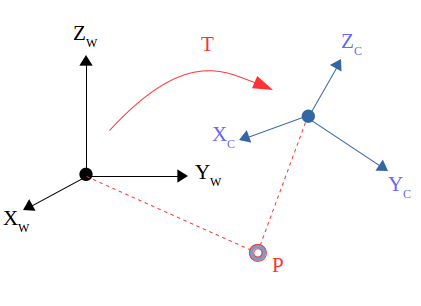
\includegraphics[scale=0.5]{./fig/wcT.png}
\caption{Transformation between coordinate systems}
\label{fig:wcT}
\end{figure}

One euclidean transformation consists of rotation and translation. First we consider rotation, we assume that one orthonormal basis $(e_1, e_2, e_3)$ after rotating becomes $(e_1^{\prime}, e_2^{\prime}, e_3^{\prime})$. In this way, for one same vector \textit{a}(this vector does not move!), the coordinates of vector \textit{a} in both system are $\begin{bmatrix} a_1,& a_2,& a_3 \end{bmatrix}^T$ and $\begin{bmatrix} a_1^{\prime}, & a_2^{\prime}, & a_3^{\prime} \end{bmatrix}^T$. According to the definition of coordinate we get:

\begin{equation*}\label{equet1}
 \begin{bmatrix} e_1 & e_2 & e_3 \end{bmatrix} 
 \begin{bmatrix} a_1 \\ a_2 \\ a_3 \end{bmatrix}
 = 
     \begin{bmatrix} e_1^{\prime} & e_2^{\prime} & e_3^{\prime} \end{bmatrix} 
     \begin{bmatrix} a_1^{\prime} \\ a_2^{\prime} \\ a_3^{\prime} \end{bmatrix}             
\end{equation*}

In order to describe the relationship of both coordinate systems, the above equation should multiply by $\begin{bmatrix} e_1^T \\ e_2^T \\ e_3^T \end{bmatrix}$ on both left and right sides, and we get a unit matrix on the left side:

\begin{equation}\label{eq:equet2}
 \begin{bmatrix} a_1 \\ a_2 \\ a_3 \end{bmatrix}
 = 
     \begin{bmatrix} e_1^Te_1^{\prime} & e_1^Te_2^{\prime} & e_1^Te_3^{\prime}\\
                     e_2^Te_1^{\prime} & e_2^Te_2^{\prime} & e_2^Te_3^{\prime}\\
                     e_3^Te_1^{\prime} & e_3^Te_2^{\prime} & e_3^Te_3^{\prime}
     \end{bmatrix}      
     \begin{bmatrix} a_1^{\prime} \\ a_2^{\prime} \\ a_3^{\prime} \end{bmatrix}             
 = Ra^{\prime}    
\end{equation}

So the matrix \textit{R} from equation \ref{eq:equet2} is called \textbf{rotation matrix}. We can find that the rotation matrix is composed of the inner product of two sets of orthonormal bases, it represents the transformation relationship of one same vector before and after rotating. we can use rotation matrix to describe camera rotation.

In addition to rotation there is also translation in euclidean transformation. One vector \textit{a} in world coordinate system becomes \textit{$a^{\prime}$} after one time rotation and one time translation \textit{t}, we can combine both rotation and translation as:

\begin{equation*}
a^{\prime} = Ra + t
\end{equation*}

Through the above formula, we describe coordinate transformation with rotation matrix \textit{R} and translation vector \textit{t} in euclidean space completely. 


\subsection{Elemental rotation matrix}
A elemental rotation is a rotation about one of the axes of a coordinate system. The following elemental rotation matrix rotates vectors by an angle $\alpha$ about the x-axis in three dimensions and the right-hand rule is used.

\texttt{Right-hand rule}: right thumb points along the axis of rotation in the positive direction, and the direction of the rest curved fingers corresponds to the positive rotation direction.

\begin{figure}[h]
\centering
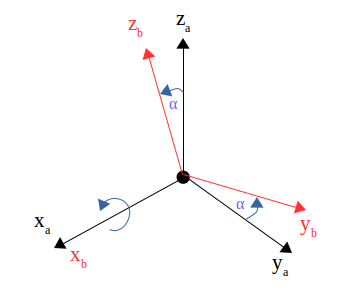
\includegraphics[scale=0.5]{./fig/rotationx.png}
\caption{Rotation about x-axis by angle $\alpha$}
\label{fig:rotationx}
\end{figure}

\begin{equation*}
R_x(\alpha) = R(x;\alpha)
      = \begin{bmatrix} 1 & 0 & 0\\
                        0 & cos(\alpha) & -sin(\alpha)\\
                        0 & sin(\alpha) & cos(\alpha) \end{bmatrix}                
\end{equation*}

Analog formulas also work for the elemental rotation matrix by an angle $\beta$, $\gamma$ about the \textit{y}-axis and \textit{z}-axis in 3D.
\begin{equation*}
R_y(\beta) = R(y;\beta)
      = \begin{bmatrix} cos(\beta) & 0 & sin(\beta)\\
                        0 & 1 & 0\\
                        -sin(\beta) & 0 & cos(\beta) \end{bmatrix}                
\end{equation*}
 
\begin{equation*}
R_z(\gamma) = R(z;\gamma)
      = \begin{bmatrix} cos(\gamma) & -sin(\gamma) & 0\\
                        sin(\gamma) & cos(\gamma) & 0\\
                        0 & 0 & 1 \end{bmatrix}                
\end{equation*}

\subsection{Euler angles}
The Euler angles are three angles to describe the orientation of a rigid body with respect to a fixed coordinate system. They can also represent the orientation of a mobile frame of reference in physics or the orientation of a general basis in 3-dimensional linear algebra. Any orientation can be achieved by composing three elemental rotations, i.e. rotations about the axes of a coordinate system. Euler angles can be defined by three of these rotations\cite{wiki_ea}.
% WIKI https://en.wikipedia.org/wiki/Euler_angles

In this thesis we denote euler angles as $\alpha$, $\beta$, $\gamma$

The three elemental rotations may be extrinsic (rotations about the axes xyz of the original coordinate system, which is assumed to remain motionless), or intrinsic (rotations about the axes of the rotating coordinate system XYZ, solidary with the moving body, which changes its orientation after each elemental rotation)\cite{wiki_ea}.
% WIKI https://en.wikipedia.org/wiki/Euler_angles

In general, euler angels can be divided in two groups(Proper Euler angles and Tait-Bryan angles):

\begin{itemize}
\item Proper Euler angles:

\begin{center}
    \begin{tabular}{ | l | l | l | p{5cm} |}
    \hline
      & Intrinsic rotations & Extrinsic rotations\\ \hline 
    1 & $z-x^{\prime}-z^{\prime\prime}$ & $z-x-z$ \\ \hline
    2 & $x-y^{\prime}-x^{\prime\prime}$ & $x-y-x$ \\ \hline
    3 & $y-z^{\prime}-y^{\prime\prime}$ & $y-z-y$ \\ \hline
    4 & $z-y^{\prime}-z^{\prime\prime}$ & $z-y-z$ \\ \hline
    5 & $x-z^{\prime}-x^{\prime\prime}$ & $x-z-x$ \\ \hline
    6 & $y-x^{\prime}-y^{\prime\prime}$ & $y-x-y$ \\ \hline
    \end{tabular}
\end{center}

\item Tait-Bryan angles(Tait-Bryan angles are also called yaw, pitch, and roll)

\begin{center}
    \begin{tabular}{ | l | l | l | p{5cm} |}
    \hline
      & Intrinsic rotations & Extrinsic rotations\\ \hline 
    1 & $x-y^{\prime}-z^{\prime\prime}$ & $x-y-z$ \\ \hline
    2 & $y-z^{\prime}-x^{\prime\prime}$ & $y-z-x$ \\ \hline
    3 & $z-x^{\prime}-y^{\prime\prime}$ & $z-x-y$ \\ \hline
    4 & $x-z^{\prime}-y^{\prime\prime}$ & $x-z-y$ \\ \hline
    5 & $z-y^{\prime}-x^{\prime\prime}$ & $z-y-x$ \\ \hline
    6 & $y-x^{\prime}-z^{\prime\prime}$ & $y-x-z$ \\ \hline
    \end{tabular}
\end{center}
\end{itemize}

\begin{equation*}
 \text{Proper Euler angles} 
 \left\{
 \begin{aligned}
        \text{Intrinsic rotations: $\overbrace{R = Z_1(\alpha)X_2(\beta)Z_3(\gamma)}^\text{post-multiply: $Z_1 \to X_2' \to Z_3''$}$}\\
        \text{Extrinsic rotations: $\underbrace{R = Z_3(\alpha)X_2(\beta)Z_1(\gamma)}_\text{pre-multiply: $Z_1 \to X_2 \to Z_3$}$}
 \end{aligned}
 \right.\
 \qquad
\end{equation*}

\begin{equation*}
 \text{Tait Bryan angles} 
 \left\{
 \begin{aligned}
        \text{Intrinsic rotations: $\overbrace{R = X_1(\alpha)Y_2(\beta)Z_3(\gamma)}^\text{post-multiply: $X_1 \to Y_2' \to Z_3''$}$}\\
        \text{Extrinsic rotations: $\underbrace{R = X_3(\alpha)Y_2(\beta)Z_1(\gamma)}_\text{pre-multiply: $Z_1 \to Y_2 \to X_3$}$}
 \end{aligned}
 \right.\
 \qquad
\end{equation*}

There are two interpretations for chained rotations:
\begin{itemize}
\item pre-multiply: $R = (R_n \cdot (R_{n-1} \cdot ... \cdot (R_2 \cdot R_1))))$, rotation in the order 1, 2, ...,n-1, n
\item post-multiply: $R = (((R_n \cdot R_{n-1}) \cdot ...R_2) \cdot R_1)$, rotation in the order n, n-1, ..., 2, 1
\end{itemize}

Sometimes, all kinds of sequences from \textit{Proper Euler angles} and \textit{Tait-Bryan angles} are called "Euler angles". In this thesis we give a example of derivation for \textit{Proper Euler angles, intrinsic rotations}:

\begin{equation}
\begin{aligned}
R &= R(z;\alpha)R(y;\beta)R(z;\gamma)
  = \begin{bmatrix} R_{11} & R_{12} & R_{13}\\
                     R_{21} & R_{22} & R_{23}\\
                     R_{31} & R_{32} & R_{33} \end{bmatrix} \\                  
      &= \begin{bmatrix} cos(\alpha)cos(\beta)cos(\gamma)-sin(\alpha)sin(\gamma) & -cos(\alpha)cos(\beta)sin(\gamma)-sin(\alpha)cos(\gamma) & cos(\alpha)sin(\beta)\\
                         sin(\alpha)cos(\beta)cos(\gamma)+cos(\alpha)sin(\gamma) & -sin(\alpha)cos(\beta)sin(\gamma)+cos(\beta)cos(\gamma)  & sin(\alpha)sin(\beta) \\
                         -sin(\beta)cos(\gamma) & sin(\theta)sin(\gamma) & cos(\beta) \end{bmatrix}   
\end{aligned}                   
\end{equation}

\subsection{Transform matrix and homogeneous matrix representation}
In our case, we use rigid transformation to describe the 3D spacial transformation of one spacial point between two different coordinate systems, which is shown in figure \ref{fig:rt}.

\begin{figure}[h]
\centering
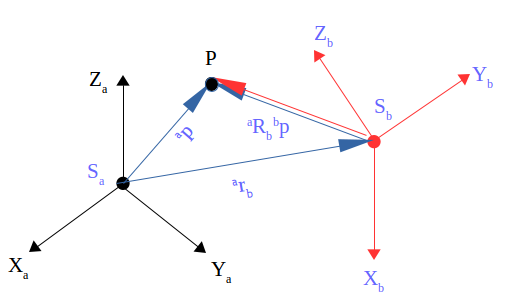
\includegraphics[scale=0.5]{./fig/rt.png}
\caption{Transformation from $S_a$ to $S_b$}
\label{fig:rt}
\end{figure}

And the transformation of point \textit{P} from $S_a$ to $S_b$ is:
\begin{align}\label{eq:equTM1}
\Aboxed{ \tensor*[^a]{p}{} = \tensor*[^a]{r}{_b} + \tensor*[^a]{R}{_b}\tensor*[^b]{p}{}}
\end{align}

\begin{itemize}
\item $\tensor*[^a]{p}{} \in \mathbb{R}^{3}$: P coordinate in system $S_a$
\item $\tensor*[^b]{p}{} \in \mathbb{R}^{3}$: P coordinate in system $S_b$
\item $\tensor*[^a]{r}{_b} \in \mathbb{R}^{3}$: translation-vector
\item $\tensor*[^a]{R}{_b} \in \mathbb{R}^{3\times3}$: rotation between $S_a$ and $S_b$
\end{itemize}

Equation \ref{eq:equTM1} represents the rotation and translation in euclidean space. But there is still a little problem: the transformation is not linear. We assume that we make two times rotations continuously: $R_1, t_1$ and $R_2, t_2$:

\begin{align*}\label{eq:equTM2}
     b = R_1a + t_1, c = R_2a + t_2               
\end{align*}

But the transformation from $a$ to $c$ is:

\begin{equation*}
     c = R_2(R_1a + t_1) + t_2            
\end{equation*}

This kind of form is too complicated after many times transformations. We turn the n-dimensional euclidean space from $R^n$ to $n+1$-dimensional by adding 1 at the end of the n-dimensional vector. It is called homogeneous coordinate.


\begin{equation*}
     \begin{bmatrix} x^{\prime} \\ 1 \end{bmatrix}
     =
     \begin{bmatrix} R & t\\
                     0^{T} & 1 \end{bmatrix}
     \begin{bmatrix} x \\ 1 \end{bmatrix}
     = T    
     \begin{bmatrix} x \\ 1 \end{bmatrix}                        
\end{equation*}

The matrix \textbf{T} is called \textbf{Transform Matrix}. Now we get a linear transformation which additionally fulfills the requirements of additivity and homogeneity, this matrix representation is easier to use. Through matrix product of the respective homogeneous matrices we can compute the concatenation of multiple rigid transformations. 


\chapter{Camera Model}
\label{chap:Camera Model}

The process of the camera mapping the coordinate points(the unit is meter) in the 3D world to the 2D image plane(the unit is pixel) can be described by a geometric model. There are many different models. The simplest of them is called the pinhole model. The pinhole model is a very common and effective model, it describes a beam of light after passing through the pinhole, its projection onto the image plane.

Now let's build a geometrically model for this simple pinhole model, which is shown in figure \ref{fig:pinhole_camera_model}. 

\begin{figure}[h!]
  \centering
  \begin{subfigure}[b]{0.6\linewidth}
    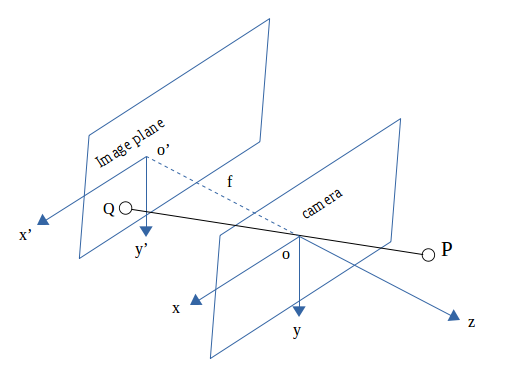
\includegraphics[width=\linewidth]{./fig/pinhole_camera.png}
    \caption{Camera coordinate system O-x-y-z}
  \end{subfigure}
  \begin{subfigure}[b]{0.3\linewidth}
    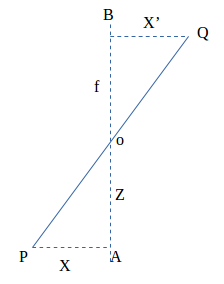
\includegraphics[width=\linewidth]{./fig/similar_triangles.png}
    \caption{Similar triangles}
  \end{subfigure}
  \caption{Pinhole camera model}
  \label{fig:pinhole_camera_model}
\end{figure}

\begin{figure}[h]
\centering
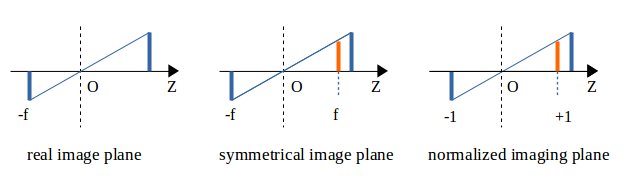
\includegraphics[scale=0.5]{./fig/3planes.png}
\caption{Real image plane, symmetrical image plane and normalized imaging plane}
\label{fig:3planes}
\end{figure}

We assume that o-x-y-z is camera coordinate system, z axis is pointing to the front of the camera, x axis is pointing to the right and y axis is pointing to down. The camera's optical center is \textit{o}, which is also the pinhole in the pinhole model. The real-world spatial point \textit{P} through the small pinhole is projected on physical image plane, the image point is \textit{Q}. We can assume that cartesian coordinate of \textit{P} is $\begin{bmatrix} X,Y,Z \end{bmatrix}^T$, \textit{Q} is $\begin{bmatrix} X',Y',Z' \end{bmatrix}^T$ and we assume that the distance from physical image plane to pinhole \textit{f}(camera focal length). Then, according to the triangle similarity theorems, we get equation \ref{eq:erla1}:

\begin{align}\label{eq:erla1}
&\frac{Z}{f} = -\frac{X}{X'} = -\frac{Y}{Y'}
\end{align}
The negative sign in equation \ref{eq:erla1} indicates that the image is inverted. In order to simplify this model, we can move the image plane to the front of the camera symmetrically, on the same side of the camera coordinate system together with the 3D spatial point. Now we can eliminate the negative sign as shown in figure \ref{fig:3planes}, make the equation more concise:
\begin{align}\label{eq:erla2}
&\frac{Z}{f} = \frac{X}{X'} = \frac{Y}{Y'}
\end{align}

After reforming equation \ref{eq:erla2}, we get the following equation which is equal to equation \ref{eq:erl5}(we will detailed explain the relationship between camera coordinate system and image plane coordinate system in section \ref{subsec:ccs_ics}):
\begin{equation}\label{eq:erla3}
 \left.\begin{aligned}
        X'=f\frac{X}{Z}\\
        Y'=f\frac{Y}{Z}
       \end{aligned}
 \right.
  \text{}
\end{equation}
Next the four plane coordinate systems in pinhole camera model and relationship between them would be introduced in the following sections:
\begin{enumerate}
\item Pixel plane coordinate system(u,v)
\item Image plane coordinate system(x,y)
\item Camera coordinate system($X_c,Y_c,Z_c$)
\item World coordinate system($X_w,Y_w,Z_w$)
\end{enumerate}

\section{The relationship between pixel plane coordinate system and image plane coordinate system}
Before determining their relationship, we can assume that the physical dimensions of each pixel in the u-axis and v-axis directions are dx and dy. Based on their model from figure \ref{fig:image_cs} we can derive the following formula:\\
\begin{align}\label{eq:erl1}
u & = \frac{x}{dx}+u_0
\end{align}
\begin{align}\label{eq:erl2}
v & = \frac{y}{dy}+v_0
\end{align}

\begin{figure}[h]
\centering
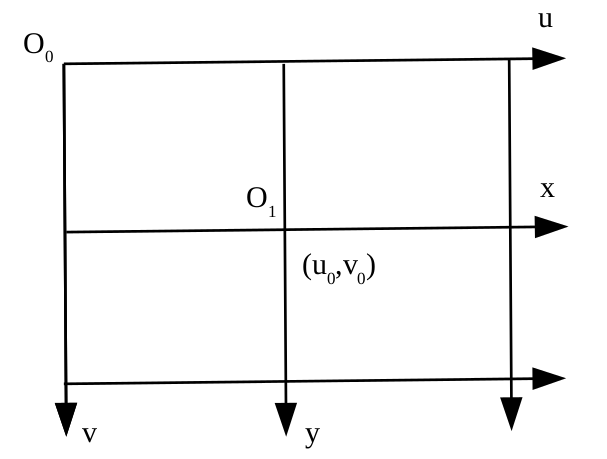
\includegraphics[scale=0.5]{./fig/image_cs.png}
\caption{Image plane coordinate system}
\label{fig:image_cs}
\end{figure}

dx, dy, u0, v0 are the parameters that we assume. dx, dy represent the actual size of the pixel on the light sensor chip. It is connected to the pixel coordinate system and the real size coordinate system. u0, v0 is the center of the image plane.

We can use the knowledge of linear algebra to represent equation \eqref{eq:erl1} and \eqref{eq:erl2} in matrix form:

\begin{equation}\label{eq:erl3}
\begin{bmatrix} u \\ v \\ 1 \end{bmatrix}
      = \begin{bmatrix} \frac{1}{dx} & 0 & u_0\\
                        0 & \frac{1}{dy} & v_0\\
                        0 & 0 & 1 \end{bmatrix}
        \begin{bmatrix} x \\ y \\1 \end{bmatrix}                 
\end{equation}

\section{The relationship between camera coordinate system and world coordinate system}

The relationship between these two coordinate systems we can rotate matrix \textit{R} and translation matrix \textit{t} to get the following relationship:
\begin{equation}\label{eq:erl4}
\begin{bmatrix} X_C \\ Y_C \\ Z_C \\ 1 \end{bmatrix}
      = \begin{bmatrix} R & t \\
                        0^T & 1 \end{bmatrix}
        \begin{bmatrix} X_W \\ Y_W \\ Z_W \\ 1 \end{bmatrix}                 
\end{equation}
In this equation, $R \in \mathbb{R}^{3\times3}$ rotates corresponding axes of each frame into each other and \textit{R} is orthogonal($R^TR = RR^T = I$), $t \in \mathbb{R}^{3\times1}$ defines relative positions of each frame.

\section{The Relationship between camera coordinate system and image plane coordinate system}
\label{subsec:ccs_ics}

In figure \ref{fig:ccs}, $O-X_CY_CZ_C$ is camera coordinate system and $o_1-xy$ is image plane coordinate system. According to the principle of triangle similarity theorems, we can derive following equations:

\begin{equation}\label{eq:erl5}
 \left.\begin{aligned}
        \frac{x}{f}=\frac{X_C}{Z_C}\\
        \frac{y}{f}=\frac{Y_C}{Z_C}
       \end{aligned}
 \right\} \Rightarrow
  \text{}
   \left\{\begin{aligned}
        Z_C \cdot x=f \cdot X_C\\
        Z_C \cdot y=f \cdot Y_C
       \end{aligned}
 \right.
  \text{}
\end{equation}

Also we can use the matrix form to represent this equations:
\begin{equation}\label{eq:erl6}
Z_C \begin{bmatrix} x \\ y \\ 1 \end{bmatrix}
      = \begin{bmatrix} f & 0 & 0 & 0 \\
                        0 & f & 0 & 0 \\
                        0 & 0 & 1 & 0 \\ \end{bmatrix}
        \begin{bmatrix} X_C \\ Y_C \\ Z_C \\ 1 \end{bmatrix}                 
\end{equation}

\begin{figure}[h]
\centering
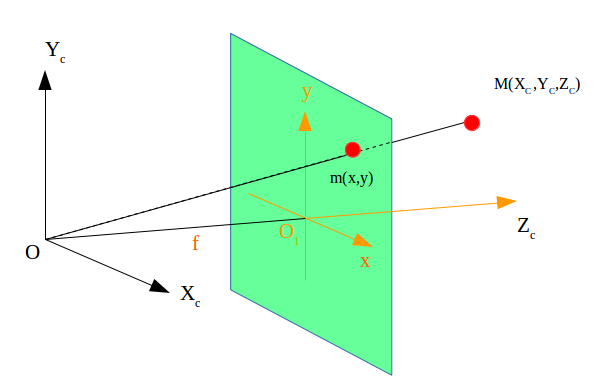
\includegraphics[scale=0.5]{./fig/ccs.png}
\caption{Image projection relationship}
\label{fig:ccs}
\end{figure}

And we can get the new formula from equations \ref{eq:erl3}, \ref{eq:erl4} and \ref{eq:erl6}:
\begin{equation}\label{eq:erl7}
Z_C \begin{bmatrix} u \\ v \\ 1 \end{bmatrix}
      = \underbrace{  
        \begin{bmatrix} \frac{1}{dx} & 0 & u_0\\
                        0 & \frac{1}{dy} & v_0\\
                        0 & 0 & 1 \end{bmatrix}
        \underbrace{                   
        \begin{bmatrix} f & 0 & 0 & 0 \\
                        0 & f & 0 & 0 \\
                        0 & 0 & 1 & 0 \\ \end{bmatrix}
        \underbrace{                 
        \begin{bmatrix} R & t \\
                        0^T & 1 \end{bmatrix}                                          
        \begin{bmatrix} X_W \\ Y_W \\ Z_W \\ 1 \end{bmatrix}
        }_\text{camera and world}    
        }_\text{projection relationship} 
        }_\text{pixel and image}                  
\end{equation}
So the camera intrinsic parameters can be described as a matrix \textit{K}:
\begin{equation}\label{eq:erl8}
K = \begin{bmatrix} f_x & 0 & u_0 & 0 \\
                    0 & f_y & v_0 & 0 \\
                    0 & 0 & 1 & 0 \\ \end{bmatrix}
  =
    \begin{bmatrix} \frac{1}{dx} & 0 & u_0\\
                     0 & \frac{1}{dy} & v_0\\
                     0 & 0 & 1 \end{bmatrix}                 
    \begin{bmatrix} f & 0 & 0 & 0 \\
                    0 & f & 0 & 0 \\
                    0 & 0 & 1 & 0 \\ \end{bmatrix}                  
\end{equation}
And \textit{R}, \textit{t} are the extrinsic parameters which denote the coordinate system transformations from 3D world coordinates to 3D camera coordinates. The extrinsic matrix can be described as:
$ \begin{bmatrix} R & t\\
                0^T & 1 \end{bmatrix}                  
$. Compared to the constant camera internal parameters, the extrinsic parameters will change with camera movement, \textit{R} and \textit{t} also denote the position of robot.

\begin{figure}[h]
\centering
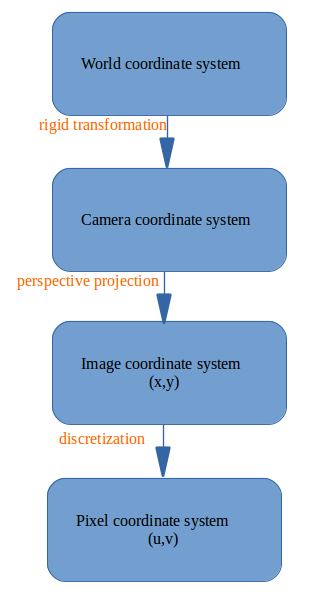
\includegraphics[scale=0.5]{./fig/4process.png}
\caption{Four coordinate systems and their relationships}
\label{fig:4process}
\end{figure}

\section{Camera distortion and image}
In geometric optics, distortion is a deviation from rectilinear projection; a projection in which straight lines in a scene remain straight in an image. It is a form of optical aberration\cite{wiki_do}.
% https://en.wikipedia.org/wiki/Distortion_(optics) 

We do not consider the camera distortion in this thesis.

In mathematics images can be described by a matrix. In the computer, they occupy a continuous disk or memory space and they can be represented by a two-dimensional array. Figure \ref{fig:image} shows a image, which height is 480 pixels and width is 640 pixels:
\begin{figure}[h]
\centering
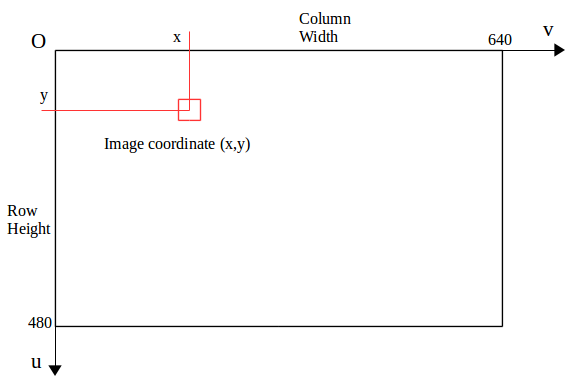
\includegraphics[scale=0.5]{./fig/image.png}
\caption{Image coordinate with 480 height and 640 width}
\label{fig:image}
\end{figure}


\chapter{Non-linear Optimization}
\label{chap:Non_linear_Optimization}

In the previous chapters, we introduce the function about camera model, and we know that we can use the transformation matrix \textbf{T} to describe camera pose. The measured equation is given by the camera's image model, the intrinsic parameters are fixed with the camera, but the extrinsic parameters are the pose of camera.

However, because of the noises, the real function and the measured function must be not exactly equal. Although the camera can be perfectly fitted with the pinhole model, but unfortunately, the data which we get is usually affected by various unknown noises. Even if we have a high-precision camera, the real function and measured function can only be approximately equal. So we have this question: how to make a camera pose estimation from noisy data accurately? This section will introduce how to handle noise data through optimization.

\section{Gradient descent method}

\textbf{Gradient descent} is also known as \textbf{steepest descent}, is first-order iterative optimization algorithm to find the minimum of a function.

\textbf{Derivative:}\\

\begin{figure}[h]
\centering
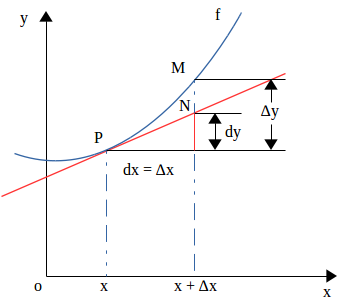
\includegraphics[scale=0.5]{./fig/derivative.png}
\caption{Derivative}
\label{fig:derivative}
\end{figure}

\begin{equation*}
f^{\prime}(x_0) = \lim_{\Delta x \to 0} \frac{\Delta y}{\Delta x} = \lim_{\Delta x \to 0} \frac{f(x_0 + \Delta x) - f(x_0)}{\Delta x}      
\end{equation*}

\textbf{Partial Derivative:}\\

\begin{equation*}
 \frac{\partial }{\partial x_j}f(x_0,x_1,\dots,x_n)= \lim_{\Delta x \to 0} \frac{\Delta y}{\Delta x} = \lim_{\Delta x \to 0} 
 \frac{f(x_0, \dots ,x_j + \Delta x,\dots,x_n) - f(x_0, \dots ,x_j,\dots,x_n)}{\Delta x}      
\end{equation*}

The derivative and the partial derivative are essentially same. Intuitively, the partial derivative is the rate of change of the function at a certain point along the positive direction of the coordinate axis. The partial derivative is the derivative with respect to one of the variables in a multivariate function.

\textbf{Directional Derivative:}\\

\begin{align*}
 \frac{\partial }{\partial l}f(x_0,x_1,\dots,x_n)&= \lim_{\rho \to 0} \frac{\Delta y}{\Delta x} \\
 &= \lim_{\rho \to 0} 
 \frac{f(x_0+\Delta x_0, \dots ,x_j + \Delta x_j,\dots,x_n+\Delta x_n) - f(x_0, \dots ,x_j,\dots,x_n)}{\rho}     \\
  \rho &= \sqrt{(\Delta x_0)^2 + \dots+(\Delta x_j)^2+\dots+(\Delta x_n)^2}
\end{align*}

In the definition of the preceding derivative and partial derivative, the change rate of the function is discussed along the positive direction of the coordinate axis. Then when we discuss the rate of change of the function in any direction, it also leads to the definition of the directional derivative, that is, the derivative value of a certain point in a direction of approach.

We must not only know the rate of change of the function in the positive direction of the coordinate axis (that is, the partial derivative), but also try to find the rate of change of the function in other specific directions. The directional derivative is the rate of change of the function in other specific directions.

\textbf{Gradient:}\\

\begin{equation*}
\mathbf{grad}f(x_0,x_1,\dots,x_n) = (\frac{\partial f}{\partial x_0},\dots,\frac{\partial f}{\partial x_j},\dots,\frac{\partial f}{\partial x_n})      
\end{equation*}

The gradient of a function at a point is such a vector whose direction is the same as the direction in which the maximum directional derivative, and its modulus is the maximum of the directional derivative.

\textbf{Gradient Descent:}\\

\begin{figure}[h]
\centering
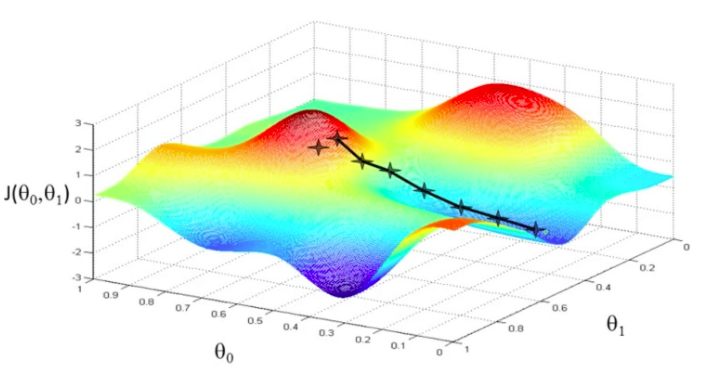
\includegraphics[scale=0.5]{./fig/gradient_descent.png}
\caption{Minimize cost function $J(\theta_0,\theta_1)$ with gradient descent}
\label{fig:gradient_descent}
\end{figure}

Since at some point in the variable space, the function has the greatest rate of change along the gradient direction, then when optimizing the objective function, it is natural to decrease the function value along the direction of the negative gradient to achieve our optimization goal.

\begin{equation*}
\mathbf{grad}f(x_0,x_1,\dots,x_n) = (\frac{\partial f}{\partial x_0},\dots,\frac{\partial f}{\partial x_j},\dots,\frac{\partial f}{\partial x_n})      
\end{equation*}

\begin{align*}
\textbf{repeat\{}\\
x_0 &:= x_0 - \alpha\frac{\partial f}{\partial x_0} \\
& \dots  \\
x_j &:= x_j - \alpha\frac{\partial f}{\partial x_j} \\
& \dots  \\
x_n &:= x_n - \alpha\frac{\partial f}{\partial x_n} \\
\}
\end{align*}

The condition for using the gradient descent method is that the direction of gradient points to the optimal solution direction, so the gradient direction is close to the optimal solution, and the gradient is very effective information about the optimal solution. On the simpler issues such as convex function and quasi convex function, it is indeed able to satisfy this condition, so the gradient descent can work well. However, when the optimization target has a large number of local extrema, most gradient directions of the solution space no longer point to the optimal solution, so in such cases the gradient method cannot get the optimal solution any more.

\section{Non-linear least squares}
The purpose of the \textbf{least squares} method is to find the least squares of error. There are two kinds of the \textbf{least squares} method: \textbf{linear} and \textbf{non-linear}. In this thesis we only consider the \textbf{non-linear} case. We usually use iterative methods(e.g. Gradient descent method; Gauss-Newton method) to solve \textbf{non-linear least squares} problem. We update the unknown variables to get closer to the approximation solution at each step with iterative method.

\begin{align*}
 \operatorname*{min}_x \norm{f(x)}^2_2  
\end{align*}

Now recall the camera model in previous section. Assume that we have \textit{n} object points in world coordinate, the \textit{i}-th point has it's corresponding projection on a plane with normalized image coordinate $x_i = [x_i,y_i]^T$. After adding the noise $\varepsilon_i$ on the error-free image coordinates $x_i$ we get noisy measurements of the image coordinates $ \tilde{x}= x_i + \varepsilon_i$. Thus, we can solve this reprojection error $\norm{\varepsilon_i}^2_2 = \norm{\tilde{x_i} - x_i}^2_2$ of each points with \textbf{least squares} method for the optimal pose $(\hat{R},\hat{t})$\cite{dynamic_markers}
%Dynamic Markers: Optimal control point configurations for homography and pose estimation
\begin{align*}
 (\hat{R},\hat{t}) = \operatorname*{argmin}_{R,t} \sum_{i=1}^{n}\norm{\varepsilon_i}^2_2  ,\qquad n \geq 3
\end{align*}


\begin{figure}[h]
\centering
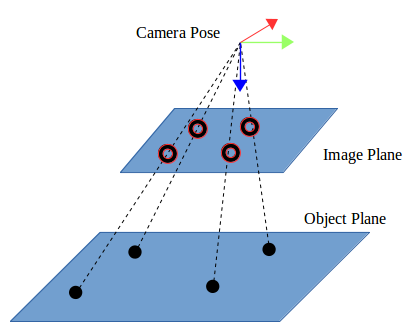
\includegraphics[scale=0.5]{./fig/least_squares.png}
\caption{Four Object points and their corresponding projection points in image plane with noisy, using least squares method to calculate the optimal camera post \textbf{R}, \textbf{t}}
\label{fig:least_squares}
\end{figure}
\chapter{Pose Estimation Algorithm}
\label{chap:Pose_Estimation_Algorithm}

%TODO
The camera pose consists of 6 degrees-of-freedom (DOF) which are made up of the rotation (roll, pitch, and yaw) and 3D translation of the camera with respect to the world.%wiki
\section{3D-2D: PnP}

\textbf{PnP(Perspective-n-Point)} is a problem of determining the pose of a calibrated camera, which given a set of n 3D points in the world coordinate system and their corresponding 2D projections in the image\cite{wiki_pnp}.
% https://en.wikipedia.org/wiki/Perspective-n-Point

There are many methods to solve \textbf{PnP} problem, for example: we can use 3 pairs of pints to determine the camera pose(\textbf{P3P}); \textbf{Direct Linear Transformation(DLT)}; \textbf{Efficient PnP(EPnP)}; \textbf{EPnP Iterative} and so on. In addition, we can also use non-linear method to build a least squares problem and solve it iteratively, that is \textbf{Bundle Adjustment}(we did not use \textbf{Bundle Adjustment} method in this thesis). 

\subsection{Direct linear transformation}
In projective geometry, \textbf{Direct linear transformation (DLT)} s an algorithm to solve a set of variables from linear equation:

\begin{align*}
   x_n = Ay_n,  & \text{ for n = 1,...,N}          
\end{align*}

where $\boldsymbol{x_n}$ and $\boldsymbol{y_n}$ are the known vectors and \textbf{A} is the matrix which contains the unknown variables need to be solved.

Considering one 3D point \textbf{P} in world, its homogeneous coordinate is $\boldsymbol{P} = (X,Y,Z,1)$. The projective points in image is $\boldsymbol{x_1} = (u_1,v_1,1)$(normalized homogeneous coordinate). At this moment, the camera pose \textbf{R}, \textbf{t} is unknown. We assume that augmented matrix 
$ \boldsymbol{\begin{bmatrix} R|t \end{bmatrix}} $ is a $3 \times 4$ matrix which contains the information of rotation and translation(it is a little different to transformation matrix \textbf{T}). We write down its expanded form:

\begin{equation}
 s \begin{bmatrix} u_1 \\ v_1 \\ 1 \end{bmatrix}
  =
    \begin{bmatrix} t_1 & t_2 & t_3 & t_4 \\
                    t_5 & t_6 & t_7 & t_8 \\
                    t_9 & t_{10} & t_{11} & t_{12} \\ \end{bmatrix}                 
    \begin{bmatrix} X \\ Y \\ Z \\ 1 \end{bmatrix}                  
\end{equation}

Use the last row of above equation to eliminate \textit{s}, we get 2 constraints:

\begin{align}
 u_1 &= \frac{t_1X + t_2Y + t_3Z + t_4}{t_9X + t_{10}Y + t_{11}Z + t_{12}}, & 
 v_1 &= \frac{t_5X + t_6Y + t_7Z + t_8}{t_9X + t_{10}Y + t_{11}Z + t_{12}}              
\end{align}

We reform the formulas and get:

\begin{align*}
 \begin{bmatrix} t_1 & t_2 & t_3 & t_4 \end{bmatrix} P -
 \begin{bmatrix} t_9 & t_{10} & t_{11} & t_{12} \end{bmatrix} u_1 &= 0,\\
 \begin{bmatrix} t_5 & t_6 & t_7 & t_8 \end{bmatrix} P -
 \begin{bmatrix} t_9 & t_{10} & t_{11} & t_{12} \end{bmatrix} v_1 &= 0.         
\end{align*}

We notice that \texttt{t} is the variable to be solved, we can find that each feature 
point(\texttt{P} and $\boldsymbol{x_1}$) provide two linear constrains about \texttt{t}.
Assume that we have N feature points all together, we can get following set of equations:

\begin{align}\label{equ:dlt}
 \begin{bmatrix} P_1^T & 0 & -u_1P_1^T\\
                 0 & P_1^T & -v_1P_1^T\\
                 \vdots & \vdots & \vdots\\
                 P_N^T & 0 & -u_NP_N^T\\
                 0 & P_N^T & -u_NP_N^T\\ \end{bmatrix} 
 \begin{bmatrix} t_1 \\ t_2 \\ t_3 \\ t_4 \\
                 t_5 \\ t_6 \\ t_7 \\ t_8 \\
                 t_9 \\ t_{10} \\ t_{11} \\ t_{12} \\ \end{bmatrix} 
 = 0.         
\end{align}

Because \texttt{t} has total 12 variables, so we need at least 6 pairs of feature points to solve this \texttt{t} responding to transformation matrix \texttt{T}. If we have more than 6 pairs of feature points, we can use \texttt{SVD} to solve overdetermined system of linear equations with least squares method.

Normally, \texttt{DLT} is a useful method to solve \textbf{PnP} problem. Also in our case we used \texttt{DLT} to solve the condition number later.
\chapter{Visual Mobile Marker Odometry}
\label{chap:Visual Mobile Marker Odometry}


Visual pose estimation and localization is very important not only for robotic applications but also useful for augmented reality. Through camera configuration(monocular,
stereoscopic or multi-camera) in different environment as well as the amount of cognition about the structure and geometry of the environment 
we can find relatively reliable solutions to this problem.

A mobile multi-robot system which was firstly introduced in \cite{kurazume1994cooperative}
can obviously speed-up and improve the accuracy of the localization
of each of the robots. In this case, the concept of \textbf{Visual Mobile Marker Odometry}(\textbf{MOMA}) was proposed with the idea of cooperative positioning for multiple robots\cite{acuna2017moma}. 
%Visual Mobile Marker Odometry

Visual pose estimation can be divided into two different categories:

\begin{enumerate}
\item Marker-based(\textbf{MA}): using some detectable visual landmarks such as fiducial markers or 3D scene models with known coordinates of its features/keypoints\cite{acuna2017moma}. 
\item Markerless(\textbf{MAL}): based on static scene features with unknown absolute coordinates in the scene(without any knowledges of 3D scene).
\end{enumerate}

In figure \ref{fig:ma_mal} are shown both cases of pose estimation.
\begin{figure}[H]
\centering
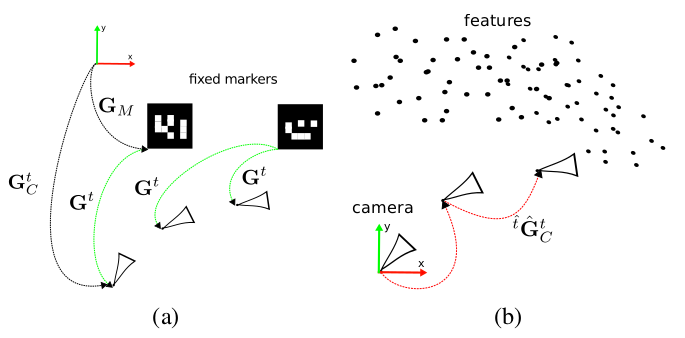
\includegraphics[scale=0.5]{./fig/ma_mal.png}
\caption{Marker-based(\textbf{MA}) pose estimation and markerless environment(\textbf{MAL-VO}) pose estimation\cite{acuna2017moma}.} 
\label{fig:ma_mal}
\end{figure}

Following we make a comparison of marker-based method and markerless method in some aspects: 
\begin{center}
   \begin{tabular}{ | l | p{5cm} | p{5cm} |}
    \hline
      & Pros & Cons\\ \hline 
    MA & not drift; reduce error from 3D to 2D only on image plane; relatively higher accuracy and lower computational complexity & require artificial markers in the environment \\ \hline
    MAL & without modification of artificial marker; can be used to detect real-world objects  & unavoidable drift; additional errors; need enough brightness and contrast of the environment   \\ \hline
    \end{tabular}
\end{center}


For our current work we only considered the case of marker-based(\textbf{MA}) method and we did the future work based on \textbf{MOMA} with two-robot caterpillar: one robot is carried with camera(monocular) as observer and the other robot is set with fiducial marker(\textbf{MA}).

The robot with camera and the robot with marker both have two states:

\begin{itemize}
\item \textbf{Mobile}: the robot is moving or permitted to move.
\item \textbf{Static}: otherwise.
\end{itemize}

The motion pattern for two-robot caterpillar is shown in figure \ref{fig:moma}. This is the background of our simulation scene.

\begin{figure}[h]
\centering
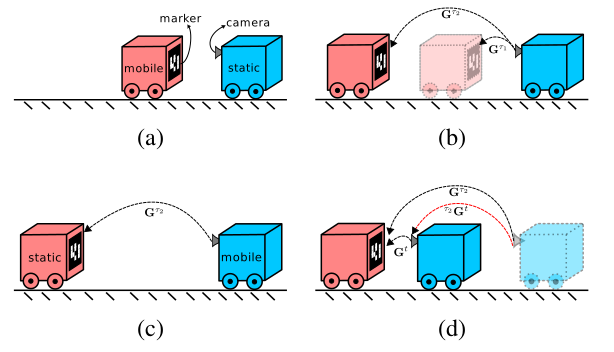
\includegraphics[scale=0.5]{./fig/moma.png}
\caption{Two-robot caterpillar. At the beginning, the robot with camera is static and the robot with marker is mobile. And then, the marker and camera exchange states which means move in turns, now the camera is mobile and marker is static. Finally, we can get the pose estimation between them\cite{acuna2017moma}.}
\label{fig:moma}
\end{figure}

\chapter{Accuracy in Optical Tracking with Fiducial Markers using Condition Number}
\label{chap:Accuracy in Optical Tracking with Fiducial Markers using Condition Number}

%New chapter
In this thesis we only consider the planar control points.
It was already proven that a square is a very stable and robust configuration for all camera poses in planar fiducial markers. Using four optimal control points with maximal equal distance to each other has the biggest influence on the improvement of accuracy\cite{dynamic_markers}.
Based on this conclusion, we also placed four control points on a planar visual fiducial marker, which are set as features in the world coordinate system.

We already know that the optical tracking with fiducial markers is commonly used in robotic applications or in augmented reality systems. One part of our work based on the \textbf{MOMA} odometry system which was shown in figure \ref{fig:moma} was to find the \textbf{accuracy function}. The \textbf{accuracy function} in our case was used to describe the specific distribution of tracking
accuracy dependent on positional relationship(such as distance or angle) between camera and marker. With this \textbf{accuracy function} we can calculate how the robot with camera and marker should be located and oriented, so we can get a optimal camera pose with minimal transformation error($\Delta R, \Delta t$).

%TODO
In previous analysis from other researchers it is already clear proven that the error in homography estimation is dependent on the singular values of the A matrix in the DLT algorithm\cite{chen2009error}.
Furthermore in \cite{dynamic_markers}
there is a research for optimal control point configurations for homography and pose estimation. The authors investigated a approach to find the optimal control point based on condition number of the A matrix in the DLT algorithm. There is a detailed derivation why we can use condition number of the A matrix in the DLT algorithm as the solution to get the optimal control point configurations and Research result
their research results indicate that there is a relationship between the rotational error, translational error of pose estimation and condition number of A matrix: They have the same trend, which means if the condition number gets larger the rotational error, translational error also get larger.
According to their research results we proposed our assumption:

\texttt{The condition number of A matrix in the DLT algorithm can be used to interpreted as the accuracy function.}
\begin{itemize}
\item If one camera pose has larger condition number we can assume that this pose estimation of this position has low accuracy.
\item If one camera pose has small condition number we can assume that this pose estimation of this position has high accuracy.
\end{itemize}

Following through building program simulations like the scheme in \cite{dynamic_markers}
,we would verify this assumption step by step.  


\section{The Accuracy function}

The accuracy function is used to describe: 

In one given detected area of a fiducial marker how accurate one position is for a given tracking situation. The ultimate goal of accuracy function is in order to
calculate how virtual objects should be located and oriented.

We wanted to find an accuracy function depending on the distance and angle between marker and camera.

\subsection{Accuracy function in past studies}
Due to the widespread use of monocular tracking systems, several groups have already worked on analyzing the accuracy of planar marker tracking systems. 
In the past studies about tracking accuracy in optimal tracking with fiducial markers are all based on experimental data, their accuracy functions were based on rotational error and translational error. Nobody actually proposed a general function to describe the tracking accuracy.  

In \cite{abawi2004accuracy} the researchers described the accuracy as a function with experimental data, they used ARToolKit to track a
single cardboard marker. They set the marker on a
stable construction as fixed and allowed a variation around the
y-axis. They mounted the camera in a mechanical jig
and adjusted in a way that the center of the lens and the
center of the marker were on the same height\cite{abawi2004accuracy}.

Their "accuracy function" assesses how accurate the tracking
parameters delivered by ARToolKit are in the specific
distance and angle to the marker if the marker was
correctly recognized in the first place.

Their results show a specific distribution of tracking
accuracy dependent on distance as well as angle
between camera and marker. Their result is shown in figure \ref{fig:acc_func}.

\begin{figure}[h]
\centering
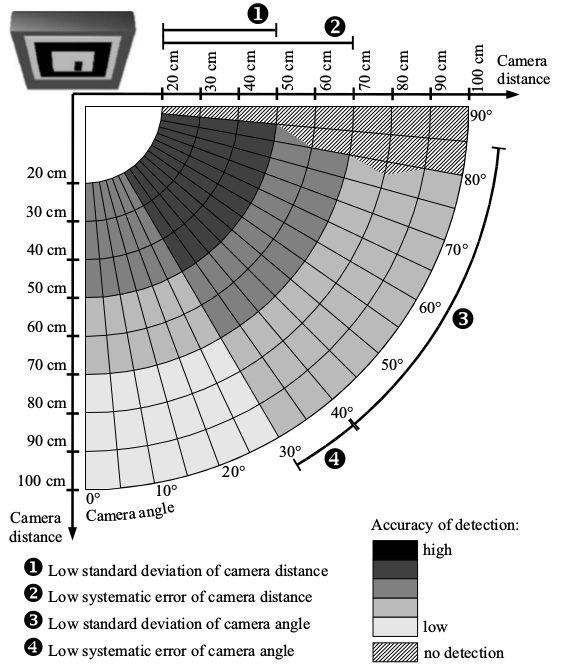
\includegraphics[scale=0.5]{./fig/acc_func.png}
\caption{Accuracy as a function of camera
distance and relative camera angle\cite{abawi2004accuracy}}
\label{fig:acc_func}
\end{figure}

Another research "Analysis of Tracing Accuracy for Single-Camera Square-Marker-Based Tracking"\cite{pentenrieder2006analysis} also presented a tracking accuracy analysis based on simulated ground truth data. Their accuracy evaluation of the visual marker based tracking system are based on the error and standard deviation. Their study only looks at the corner detection error but not consider pose estimation errors. Their experimental design follows "one-factor-at-a-time" principle and then also consider the combinations of all input factors. I also learned from this idea, which means firstly I studied the influence of \textbf{height}(distance of the marker) and \textbf{angle}(viewing angles) separately, after that I studied the combination of these influenced factors which means \textbf{height} and \textbf{angle} would be considered at the same time. They provided the following results:

\begin{itemize}
\item For larger distances the translational pose error and rotational pose error both increase. 
\item When the camera and marker form a certain small angle, it gets the smallest translational pose error and rotational pose error. But if the angle too small or the camera gradually becomes vertical to the marker, the translational pose error and rotational pose error would get bigger.
\end{itemize}

These results are shown in figure \ref{fig:Error_distance_angle} which are actually similar to the results in \cite{abawi2004accuracy}, but just in different form to represent it.

We can find that both researches \cite{abawi2004accuracy} and \cite{pentenrieder2006analysis}
were based on experimental data to describe the tracking accuracy, but they actually did not provide a "traditional function" to describe the accuracy, just like this simple form $f(x,y,z) = ax+by+cz$, where \texttt{f} is the desired accuracy function, \texttt{x}, \texttt{y}, \texttt{z} are the possible influencing factors of the accuracy function. 

\begin{figure}[H]
\centering
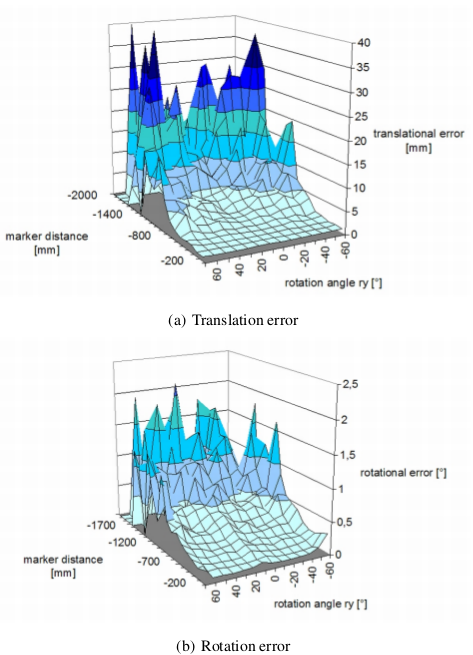
\includegraphics[scale=0.7]{./fig/Error_distance_angle.png}
\caption{Error for camera distance and rotation angle\cite{pentenrieder2006analysis}}
\label{fig:Error_distance_angle}
\end{figure}

\subsection{The desired accuracy function}
To fill this gap in this field, in our project we created the real "accuracy function", which means in the detection area of the given marker and camera, if one position coordinate is given we can obtain the information of accuracy at this corresponding position from the "accuracy function".

\begin{figure}[H]
\centering
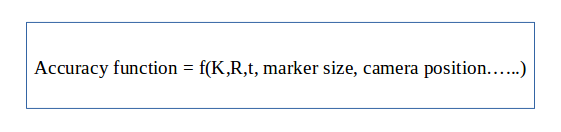
\includegraphics[scale=0.8]{./fig/acc_simple.png}
\caption{One simple example for the form of accuracy function, the influencing factors could be the camera intrinsic parameters; camera extrinsic parameters; the size of planar marker; the position of camera and so on}
\label{fig:acc_simple}
\end{figure}
%------------------------------------------
In this project we proposed the assumption that the condition number distribution can be interpreted as our desired accuracy function. 

Firstly, we convert the selected grid-based rectangle region which contains the detection region of the marker into a $m \times n$ matrix. This process is shown in figure \ref{fig:mncells}.

\begin{figure}[H]
\centering
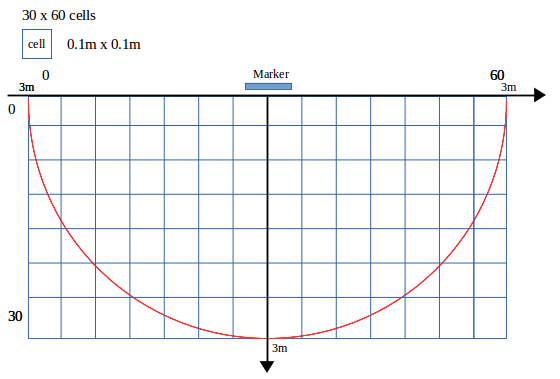
\includegraphics[scale=0.8]{./fig/mncells.png}
\caption{The detection region of the marker is defined as a semicircle with radius 3 meter, the $3m \times 6m$ rectangle region is grid-based and each cell is $0.1m \times 0.1m$, this region would be converted into a $30 \times 60$ matrix.}  
\label{fig:mncells}
\end{figure}

For each grid-cell there maybe several camera poses locate on it. Then we compute the average value \texttt{c} of all condition numbers of these camera poses fall onto the same cell, this average value \texttt{c} can be treated as the condition number of this cell. This process is shown in figure \ref{fig:cell_cn}.

\begin{figure}[H]
\centering
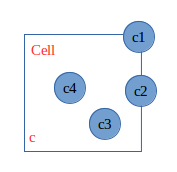
\includegraphics[scale=0.8]{./fig/cell_cn.png}
\caption{The blue square represents one cell and each blue circle represents one camera position. Condition number of this cell: $c = mean(c_1 + c_2 +c_3 + c_4)$}  
\label{fig:cell_cn}
\end{figure}

After that we can get a similar condition number distribution like the matrix shown in figure \ref{fig:conditionNum_mat}.
\begin{figure}[H]
\centering
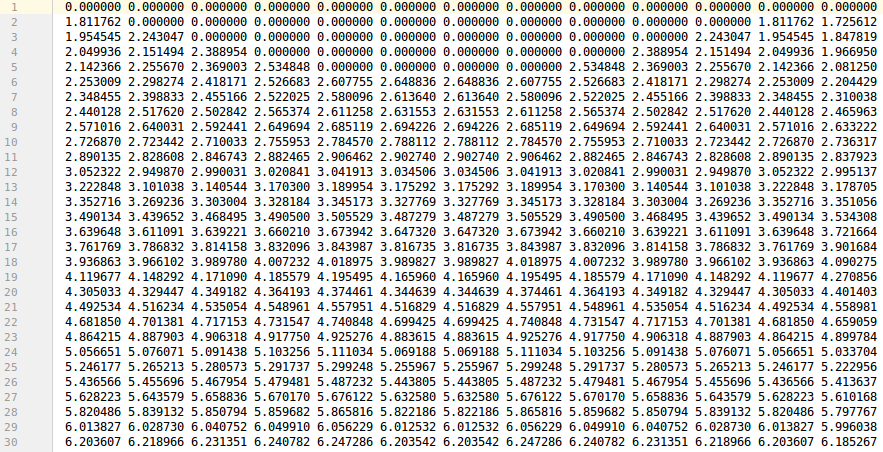
\includegraphics[scale=0.5]{./fig/conditionNum_mat.png}
\caption{An simple example of condition number distribution matrix, which is a $30 \times 60$ matrix, the above only shows part of the condition number distribution matrix}  
\label{fig:conditionNum_mat}
\end{figure}

After that if we want, we can divide the condition numbers into several degrees between the maximum and minimum, treating them as accuracy distribution. Finally, we can get the accuracy degree at given camera position. This whole precess is shown in figure \ref{fig:mc_process}.

\begin{figure}[H]
\hspace*{3cm}
\centering
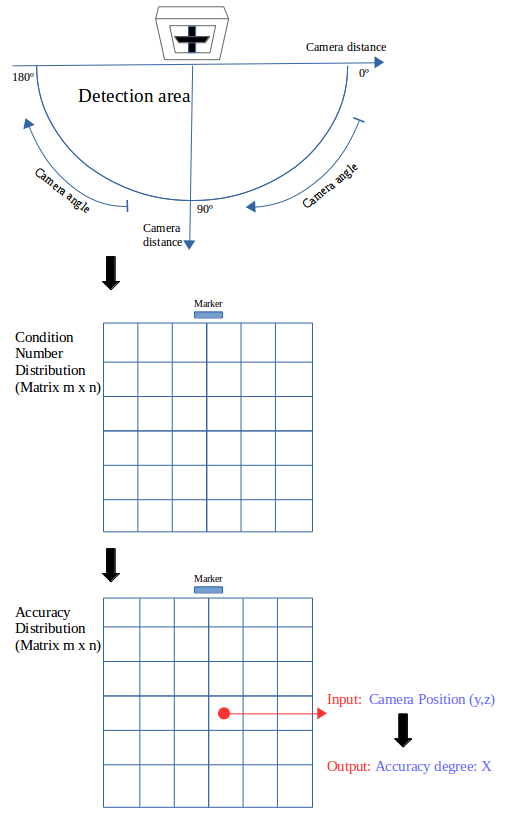
\includegraphics[scale=0.8]{./fig/mc_process.png}
\caption{Process...TODO}  
\label{fig:mc_process}
\end{figure}

From this we can find that the accuracy distribution(accuracy function) is affected by camera intrinsic, extrinsic parameters, the size of marker and the camera pose. And the key to find the accuracy function is : \texttt{Find out the condition number distribution.} 

Also the condition number distribution was used for our motion planning algorithms in chapter \ref{chap:Motion_planning}. In the following sections I will explain detailedly why the condition number distribution can be interpreted as the accuracy function and how we can get the condition number distribution in our simulations.

\subsection{Homography estimation}
\textbf{What is a homography?} 

A 2D point $(x,y)$ in the image plane can be represented as $(x_i,y_i,z_i)$ in 3D plane, where $x = \frac{x_i}{z_i}$ and $y = \frac{y_i}{z_i}$. This process is called homogeneous
representation of a 2D point. And the \textbf{homography matrix} is a non-singular $3 \times 3$ matrix which describes the linear mapping relationship between two planes in 2D homogenous coordinates(usually describes the transformation of some points in the common plane between two images, shown in figure \ref{fig:homo_es}). 

\begin{figure}[h]
\centering
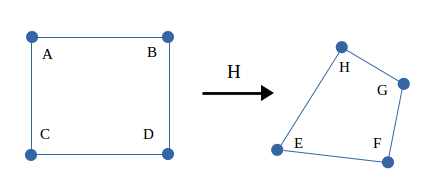
\includegraphics[scale=0.5]{./fig/homo_es.png}
\caption{Homography matrix}  
\label{fig:homo_es}
\end{figure}

We assume that there is a pair of matched feature points $p_1$ and $p_2$ in two different planes. Directly we can use homography matrix to describe the transformation between $p_1$ and $p_2$:
\begin{align*}
 p_2 = Hp_1  
\end{align*}
\begin{align*}
\begin{bmatrix} u_2 \\ v_2 \\ 1  \end{bmatrix}
=
\begin{bmatrix} h_1 & h_2 & h_3 \\
                h_4 & h_5 & h_6 \\
                h_7 & h_8 & h_9 \end{bmatrix}
\begin{bmatrix} u_1 \\ v_1 \\ 1  \end{bmatrix}
\end{align*}
where \textbf{H} is the homography matrix. We set $h_9 = 1$ and then reform the above formula:
\begin{align*}
h_1u_1 + h_2v_1 + h_3 - h_7u_1u_2 - h_8v_1u_2 &= u_2 \\
h_4u_1 + h_5v_1 + h_6 - h_7u_1v_2 - h_8v_1v_2 &= v_2 
\end{align*}

From above equations we find that there are now 8 unknowns($h_1 \sim h_8$) existed in 2 equations. In order to solve \texttt{H} we still need additional six equations, which means we need totally 4 pairs of points.

The Direct Linear Transform(DLT) is a common standard algorithm used
to solve for the homography matrix \texttt{H} given a sufficient set of corresponding point.
We notice that \texttt{H} can be changed by multiplying by an arbitrary
non-zero constant without altering the projective transformation. So usually $h_9$ should be set as $h_9 = 1$. In this case a homogeneous matrix only has 8 degrees of freedom even
though it contains 9 elements, which means we only need to solve these 8 unknown variables. From above equation we know that each pair of matched points can build one constrain for DLT. So we need 4 pairs of matched points to solve homography matrix \texttt{H}. And in our project the detected marker has 4 corner points for estimating of homography.
After estimating the homography we can get our expected rotation matrix \textbf{R} and translation vector \textbf{t} from corresponding homography matrix \textbf{H}.

\texttt{Normalizing transformations:}

For DLT algorithm the normalization of the measurements is a important step to improve the quality of the estimated homography. Normalization of the data consists of translation and scaling of image coordinates. This normalization should be carried out before applying the DLT algorithm.

Recall that the DLT formula \ref{equ:dlt} for 6 pairs of points, we can derive a similar formula for 4 pairs of points:
\begin{align}\label{equ:ah4}
 Ah = \begin{bmatrix} P_1^T & 0 & -u_1P_1^T\\
                 0 & P_1^T & -v_1P_1^T\\
                 \vdots & \vdots & \vdots\\
                 P_4^T & 0 & -u_4P_4^T\\
                 0 & P_4^T & -u_4P_4^T\\ \end{bmatrix} 
 \begin{bmatrix} t_1 \\ t_2 \\ t_3 \\ t_4 \\
                 t_5 \\ t_6 \\ t_7 \\ t_8 \\ \end{bmatrix} 
 = 0.         
\end{align}
The normalization is basically a preconditioning to decrease condition number of the matrix A(when there is noise in the measurement data, the more severe the change in the condition number, the more sensitive the method is to errors, and the less robust the method is. So low condition number of matrix \texttt{A} for our simulation is desired).
And it is already proven that the DLT algorithm is in practice invariant to similarity transformations\cite{hartley2000multiple}.

"Apart from improved accuracy of results, data normalization provides a second desirable benefit, namely that an algorithm that incorporates an initial data normalization step will be invariant with respect to arbitrary choices of the scale and coordinate origin. This is because the normalization step undoes the effect of coordinate changes, by effectively choosing a canonical coordinate frame for the measurement data.\cite{hartley2000multiple}"

For our case we also used the \texttt{isotropic scaling.} method which is also mentioned in \cite{hartley2000multiple}.
We can summarize the steps of isotropic scaling as follows:
\begin{enumerate}
\item The four image points(also the four object points) are translated so that their centroid is at the origin.
\item Then the four points are scaled so that the mean distance from the origin is $ \sqrt{2}$.
\end{enumerate}

This process is shown in figure \ref{fig:normalization}.
\begin{figure}[h]
\centering
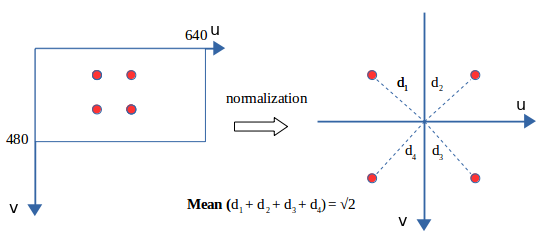
\includegraphics[scale=0.8]{./fig/normalization.png}
\caption{Normalization of 4 image points, this process can reduce condition number of matrix \texttt{A} and maximize the robustness of the DLT
homography estimation against noise}  
\label{fig:normalization}
\end{figure}

\texttt{Why is normalization essential?} %TODO

There is already a complete good answer in \cite{hartley2000multiple}. All in all we apply normalization is in order to set all entries in matrix \texttt{A} have similar magnitude and increase the robustness of accuracy function.

However, the normalization still has some disadvantages:
\begin{itemize}
\item The estimated homography depends on the similarity transforms.
\item The normalization matrices are computed from
noisy pixel measurements, and therefore sensitive to outliers.
\end{itemize}

To overcome these disadvantages a (non-iterative)method for estimating homographies does not
rely on coordinate normalization is proposed in \cite{rangarajan2009estimating} which is by avoiding normalization and instead using a \texttt{Taubin estimator}, that is unaffected by similarity transformations of the correspondences in the two views. 

In our project we will compare the results of the accuracy function for estimating homographies without normalization and with normalization.

\subsection{Connect accuracy function with condition number}
In this section I will explain why the condition number distribution can be interpreted as the accuracy function.\\

\texttt{Planar Point Configuration for Pose Estimation:}

In previous section we already introduced the pinhole camera model and the pose estimation from 3D points. And in our project we applied a planar marker to estimate the camera pose. Specially if the control points are all on a plane, we can reduce the degree of freedom of the rotational matrix \texttt{R}.(Now we can use two angles instead of three angles to represent rotational matrix \texttt{R}:
\begin{align*}
\Aboxed{R = [r_1, r_2, r_3] \to R = [r_1, r_2]}
\end{align*}
Because all control points are located on a plane, we can define a 2D subspace instead of three-dimensional coordinates in 3D world, set the Z-coordinate as 0:
\begin{align*}
X_i^W = \begin{bmatrix} X_i^W \\ Y_i^W \\ Z_i^W \end{bmatrix} \implies 
X_i^W = \begin{bmatrix} X_i^W \\ Y_i^W \\ 0 \end{bmatrix}
\end{align*}
Under the perspective projection model, through the projection matrix \texttt{P} mapping three-dimensional space points \texttt{X} onto \texttt{u} on the image plane. The transformation can be represented as following equation:  
\begin{align*}
s\overline{u} &= P\overline{X} \\
s \begin{bmatrix} u \\ v \\ 1 \end{bmatrix} &= P \begin{bmatrix} X^W \\ Y^W \\ Z^W \\ 1 \end{bmatrix} = \begin{bmatrix} p_1 & p_2 & p_3 & p_4 \end{bmatrix} \begin{bmatrix} X^W \\ Y^W \\ Z^W \\ 1 \end{bmatrix}
\end{align*}
where $\overline{u} = \begin{bmatrix} u,&v,&1 \end{bmatrix}$, $\overline{X}=\begin{bmatrix} X^W, &Y^W, &Z^W, &1 \end{bmatrix}$ are represented as homogeneous coordinates and \texttt{s} is the non-zero scale factor. We assume that plane $\pi$ is the plane where our fiducial marker are located(plane $\pi$ is the \texttt{XOY} plane of the object coordinate system). For points on the plane $\pi$, there is $Z_i = 0$, then we can get following deformation:
\begin{align*}
s \begin{bmatrix} u \\ v \\ 1 \end{bmatrix} &= P \begin{bmatrix} X^W \\ Y^W \\ 0 \\ 1 \end{bmatrix} = 
\underbrace{\begin{bmatrix} p_1 & p_2 & p_3 \end{bmatrix}}_\text{H}
 \begin{bmatrix} X^W \\ Y^W \\ 1 \end{bmatrix}
\end{align*}
where $H = \begin{bmatrix} p_1,&p_2,&p_3 \end{bmatrix}$, we can describe $\overline{X_{\pi}}$ as $\overline{X_{\pi}} = \begin{bmatrix} X^W,&Y^W,&1 \end{bmatrix}$, then we get following equation:
\begin{align}\label{equ:suhx}
s\overline{u} &= H\overline{X_{\pi}}
\end{align}

Similar to 6 pairs of points DLT algorithm derivation in previous section and in our project we used a fiducial marker with four control points(any 3 points are not collinear) on a plane. Solving equation \ref{equ:suhx} is equal to solve the following equation, which has the similar form as formula \ref{equ:ah4}:
\begin{align*}
\Aboxed{Ah = 0}
\end{align*}
\begin{align*}
A =
\begin{bmatrix} 0 & 0 & 0 & -X_1 & -Y_1 & -1 & v_1 X_1 & v_1 Y_1 & v_1 \\
                X_1 & Y_1 & 1 & 0 & 0 & 0 & -u_1 X_1 & -u_1 Y_1 & -u_1 \\
                0 & 0 & 0 & -X_2 & -Y_2 & -1 & v_2 X_2 & v_2 Y_2 & v_2 \\
                X_2 & Y_2 & 1 & 0 & 0 & 0 & -u_2 X_2 & -u_2 Y_2 & -u_2 \\
                0 & 0 & 0 & -X_3 & -Y_3 & -1 & v_3 X_3 & v_3 Y_3 & v_3 \\
                X_3 & Y_3 & 1 & 0 & 0 & 0 & -u_3 X_3 & -u_3 Y_3 & -u_3 \\
                0 & 0 & 0 & -X_4 & -Y_4 & -1 & v_4 X_4 & v_4 Y_4 & v_4 \\
                X_4 & Y_4 & 1 & 0 & 0 & 0 & -u_4 X_4 & -u_4 Y_4 & -u_4 \\
\end{bmatrix}
\end{align*}

where $A \in \mathbb{R}^{8 \times 9}$ and $h = \begin{bmatrix}
r_1^T,&r_2^T,&t^T
\end{bmatrix}^T \in  \mathbb{R}^9$.
Under additional constraint $ \norm{h} = 1$, \texttt{h} is the homography matrix with 8 unknowns.

However in the actual situation we set noisy(Gaussian distribution) for each image points, again assuming noisy measurements for image points $\widetilde{u_i} = u_i + \xi_i$, we get the matrix $\widetilde{A} = A + E$ with noise. Due to the presence of noise, in the most cases $\widetilde{A} h \neq 0$, so \texttt{h} would be estimated by minimization of $\widetilde{A} h$, due to $Ah = 0$,  this problem can be solved also by minimization of $\norm{Eh}_2^2$:
\begin{align}\label{equ:aheh}
h = argmin_h \norm{\widetilde{A}h}_2^2 = argmin_h \norm{Eh}_2^2,\quad with  \quad \norm{h} = 1
\end{align}

Solving equation \ref{equ:aheh} is actually equivalent to apply a singular value decomposition(SVD) of $\widetilde{A} = \widetilde{U}\widetilde{S}\widetilde{V}$ for this DLT algorithm, where the solution of equation \ref{equ:aheh} is $ h = \widetilde{v_9}$ with $\widetilde{v_9}$ being the right singular vector of $\widetilde{A}$, associated with the least singular value $\widetilde{s_9}$.

\begin{figure}[H]
\centering
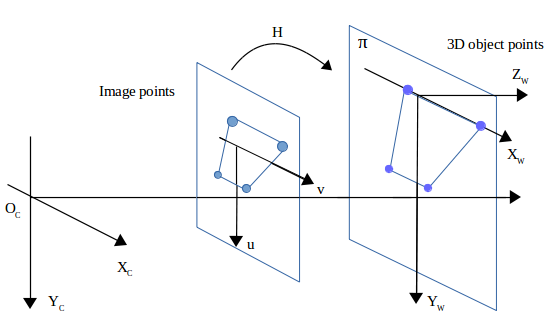
\includegraphics[scale=0.5]{./fig/H.png}
\caption{The perspective projection of the 3D plane}  
\label{fig:H}
\end{figure}

\texttt{Why is condition Number?}
 
For the linear problem, the condition number of the measurement matrix is an important factor affecting its numerical stability.

If the singular values of matrix \textit{A} are $d_1,d_2,\dotsm ,d_9(d_1 \geq d_2 \dotsm \geq d_9 = 0)$, then the condition number of matrix \textit{A} is:
\begin{align*}
c(A) = \frac{d_1}{d_8}
\end{align*}

In previous researches from \cite{abawi2004accuracy} and \cite{pentenrieder2006analysis} they described the accuracy function with the rotational error and translational error. And in \cite{dynamic_markers} there is a interesting results, when the rotational error and translational error decrease or increase, the condition number at corresponding position also becomes smaller or bigger. They have a similar trend in terms of different camera pose. Through this discovery we therefore made our assumption that we can use condition number to describe the accuracy function. And through our simulations we already verified this assumption.

In following sections I will explain how our simulations were performed.

\section{Simulation design}
\subsection{Simulation frame setup}

For the simulation the two most important objects are: \texttt{marker} and \texttt{camera}. 
In order to make simulation between marker and camera, we need to set some properties of both.
\subsubsection{Marker}
We used a square fiducial marker for camera pose estimation. More precisely the four vertices of the square marker are defined as the control points, which are then needed to project onto the camera image. Because in \cite{dynamic_markers} it was already verified that for 4 points in most cases the vertices of a square marker are the optimal control points, therefore these four vertices are represented as our detected features for camera.

We set that the center of the marker is the origin of world coordinate system($O-X_W Y_W Z_W$). And the fiducial planar marker was located on \texttt{XOY} plane in the world coordinate system. The positive direction of Z-axis points to the region where the cameras should be located on. The coordinates of the four control points under world coordinate system are:
\begin{enumerate}
\item Point 1: $(0.15,0.15)$
\item Point 2: $(0.15,-0.15)$
\item Point 3: $(-0.15,-0.15)$
\item Point 4: $(-0.15,0.15)$
\end{enumerate}
In the simulation the default size of the marker was set as $0.3m \times 0.3m$ and we set the marker as fixed at the origin of the coordinate system, of course we can change different size of the marker to fit more testing scenarios. 

The simulation scene of the planar marker is illustrated in figure \ref{fig:marker}.
\begin{figure}[H]
\centering
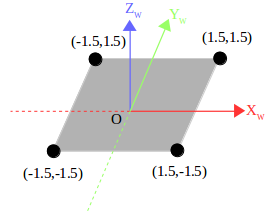
\includegraphics[scale=0.5]{./fig/marker.png}
\caption{A marker with size $0.3m \times 0.3m$, four features at each corner.}  
\label{fig:marker}
\end{figure}

  
\subsubsection{Camera}
We already introduce the camera model in previous section and it is well-known that we often use 
$\begin{bmatrix}
u & v & 1
\end{bmatrix}^T$ to represent the position of a 2D point in pixel coordinates, corresponding 
$\begin{bmatrix}
X_W & Y_W & Z_W & 1
\end{bmatrix}^T$ is used to represent the position of 3D point in world coordinate system. According to the pinhole camera model, we know the following projective mapping from world coordinate system to pixel coordinate system:
\begin{equation}
Z_C \begin{bmatrix} u \\ v \\ 1 \end{bmatrix}
      = K 
        \begin{bmatrix} R | t \end{bmatrix}                                          
        \begin{bmatrix} X_W \\ Y_W \\ Z_W \\ 1 \end{bmatrix}
\end{equation}
where \textit{K} is the intrinsic parameters and we set it's default value as
$\mathbf{K} = \begin{bmatrix} 800 & 0 & 0\\
                 0 & 800 & 240\\
                 0 & 0 &1\end{bmatrix}$, the extrinsic parameters \texttt{R} and \texttt{t} are the variables we are interested in. By setting different camera positions in our simulation we obtain different camera pose, that is the rotation matrix \texttt{R} and translation vector \texttt{t}. It is worth noting that in our project we did not consider the camera distortion problem for now. 

We set the image default size as $\mathit{640 \times 480[pixel^2]}$, through derivation of camera intrinsic parameters \texttt{K} in previous section we can easily find that parts of \texttt{K} parameters are related to the height and width of the image. Therefore if we change the size of the image, we also need to change the camera intrinsic parameters \texttt{K} correspondingly.   
 
Although we do not need to consider the camera distortion problem, in the real environment camera noise is an unavoidable factor. In order to simulate the reality of camera we set the image noise manually. For each image point we added a 2-dimensional Gaussian distribution:
\begin{python}
    def addnoise_imagePoints(self, imagePoints, mean = 0, sd = 2):
        """ Add Gaussian noise to image points
        imagePoints: 3xn points in homogeneous pixel coordinates
        mean: zero mean
        sd: pixels of standard deviation
        """
        imagePoints = np.copy(imagePoints)
        if sd > 0:
            gaussian_noise = np.random.normal(mean,sd,(2,imagePoints.shape[1]))
            imagePoints[:2,:] = imagePoints[:2,:] + gaussian_noise
        return imagePoints
\end{python}

\texttt{camera distribution:}\\
Normally each camera has a fixed detection range, in our simulation we fixed the position of planar marker, in this way we can image that each marker has a detection area just like the camera. Therefore the cameras can be treated as moved in the detection region of the marker. This idea is shown in figure \ref{fig:cm_invert}.
\begin{figure}[H]
\centering
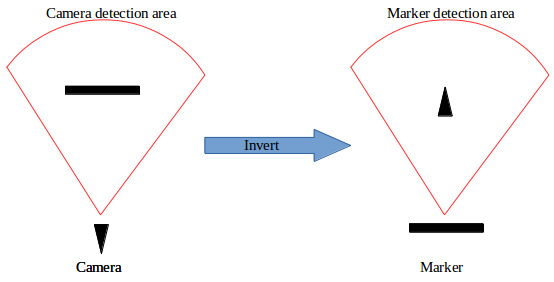
\includegraphics[scale=0.7]{./fig/cm_invert.png}
\caption{Invert camera and marker}  
\label{fig:cm_invert}
\end{figure}

Because in our situation the robot moves only on \textbf{YZ}-plane of world coordinates and the heights of the canter of the marker and camera lens always keep at the same level, this scenario is shown in figure \ref{fig:marker_camera}. Therefore we can simplify the 3D camera distribution shown in figure \ref{fig:cam3D2D}(a) into the 2D camera distribution shown in figure \ref{fig:cam3D2D}(b). 

\begin{figure}[H]
\centering
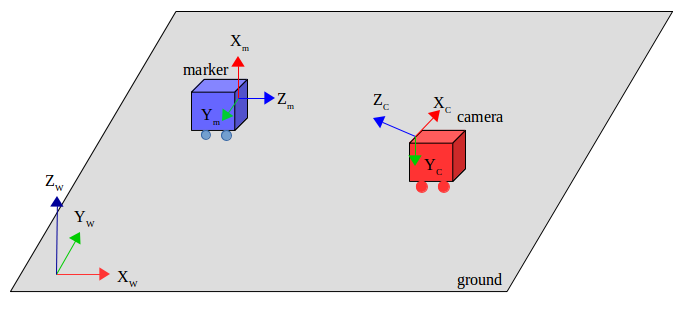
\includegraphics[scale=0.45]{./fig/marker_camera.png}
\caption{Two-robot Caterpillar}  
\label{fig:marker_camera}
\end{figure}

\begin{figure}[H]
  \centering
  \begin{subfigure}[b]{0.8\linewidth}
    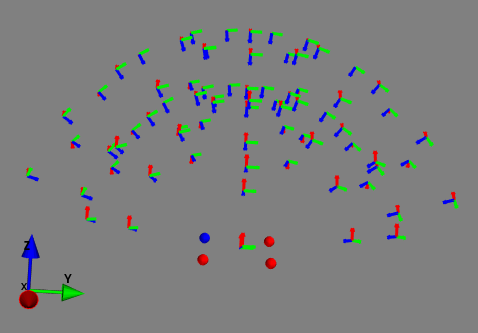
\includegraphics[width=\linewidth]{./fig/cam3D.png}
    \caption{An Example for camera distribution in 3D. The camera are distributed evenly on spheres of different radius. Each camera(positive direction of Z-axis) should look at the origin of the plane.}
  \end{subfigure}
  \begin{subfigure}[b]{0.8\linewidth}
    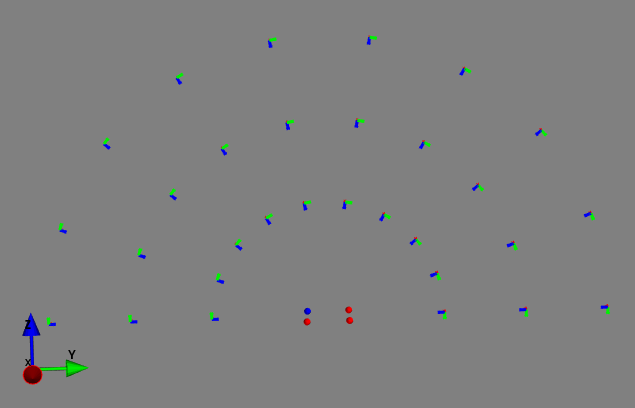
\includegraphics[width=\linewidth]{./fig/cam2D.png}
    \caption{An Example for camera distribution in 2D. The camera are distributed evenly on YZ-plane. Each camera(positive direction of Z-axis) should look at the origin of the plane. We apply this 2D case in our simulation.}
  \end{subfigure}
  \caption{Camera distribution}
  \label{fig:cam3D2D}
\end{figure}

In our simulation we set a very important rule:

\texttt{Each camera should look at the center of the planar marker!}

\subsection{Simulation approach}

A very common approach for simulations or experiments is the "one-factor-at-a-time" method\cite{wiki_ofaatm}, which means we should study only one affected factor while all others are kept constant. But this approach fails to consider the effect of multiple variable combinations on one system or on one function. So beyond this approach we also need to consider the combinations of all inputs. For example in our simulation we need to consider not only the influence of height and angle separately but also the interactions of height and angle.

Therefore we applied "one-factor-at-a-time" method at the beginning of the simulation, trying to find out some rules or clues for accuracy function, we can treat it as heuristics. On the basis of that we estimated interactions between different factors and trying to find out the final experimental conclusion from our simulation.

In our simulation we studied two important factors:
\begin{itemize}
\item \texttt{Height}: the distance between camera and marker, we can also call it \texttt{radius}. 
\item \texttt{Angle}: the angle between Z-axis of camera and marker plane.
\end{itemize}
\section{Results}
We have already pointed out that the condition number distribution can be interpreted as the accuracy function and later the condition number distribution can be used in our pathfinding. Therefore in this section we provide the results all about condition number distribution. 

Also according to the research in \cite{pentenrieder2006analysis}, our desired results are:
\begin{itemize}
\item If the angle between camera and marker plane is fixed, the closer the distance between camera and marker, the smaller the condition number is.
\item If the distance between camera and marker is fixed, the smaller the angle between camera and marker plane, the smaller the condition number is.
\end{itemize}

In previous sections we already mentioned that how important the normalization of homography is. In this part different results without normalization and with normalization would be compared detailedly. Then Therefrom we found out the best solution which is satisfied our desired results.

In order to compute the condition number distribution the object points and image points were transformed like follows in four ways: 
\begin{enumerate}
\item object points: no normalized, image points: no normalized
\item object points: regular normalized, image points: regular normalized
\begin{python} 
scale = np.sqrt(2) / meandist # Translation and scaling 
\end{python}
\item object points: regular normalized, image points: normalized
\begin{python} 
scale = 1 # Only translation, no scaling 
\end{python}
\item object points: regular normalized, image points: normalized
\begin{python}
scale = radius*np.sqrt(2) / meandist 
\end{python}

\end{enumerate}

where in the second case the \texttt{regular normalized} means the four points are scaled so that the mean distance from the origin is $ \sqrt{2}$, for the third case the four image points are only translated but not scaling, for the fourth case the four image points are scaled so that the mean distance from the origin is $ radius * \sqrt{2}$(radius is the distance from camera to marker).

In order to represent the results clearly, we used colormap \texttt{magma} form \texttt{matplotlib} library\cite{matplotlib} to represent our data set:
\begin{itemize}
\item Dark color(black) $\to$ small condition number
\item Light color(yellow) $\to$ big condition number
\end{itemize}

\begin{figure}[H]
\centering
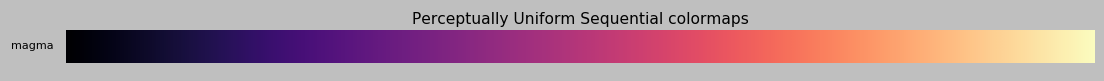
\includegraphics[scale=0.34]{./fig/magma.png}
\caption{Colormap \textit{magma} from \textit{matplotlib} library}  
\label{fig:magma}
\end{figure}
%======================================================================
\texttt{Condition number distribution without normalized homography:}

At first, we computed the condition number of each camera pose without normalization of the homography.

\begin{python}
# Compute the condition number without normalization
cond_num = gd.matrix_condition_number_autograd(*input_list, normalize = False)
\end{python} 

And we applied "one-factor-at-a-time" method that we made simulations for \texttt{angle} and \texttt{height} separately and we got the following results which are shown in figure \ref{fig:angle_height}: 

\begin{figure}[H]
  \centering
  \begin{subfigure}[b]{1.0\textwidth}
    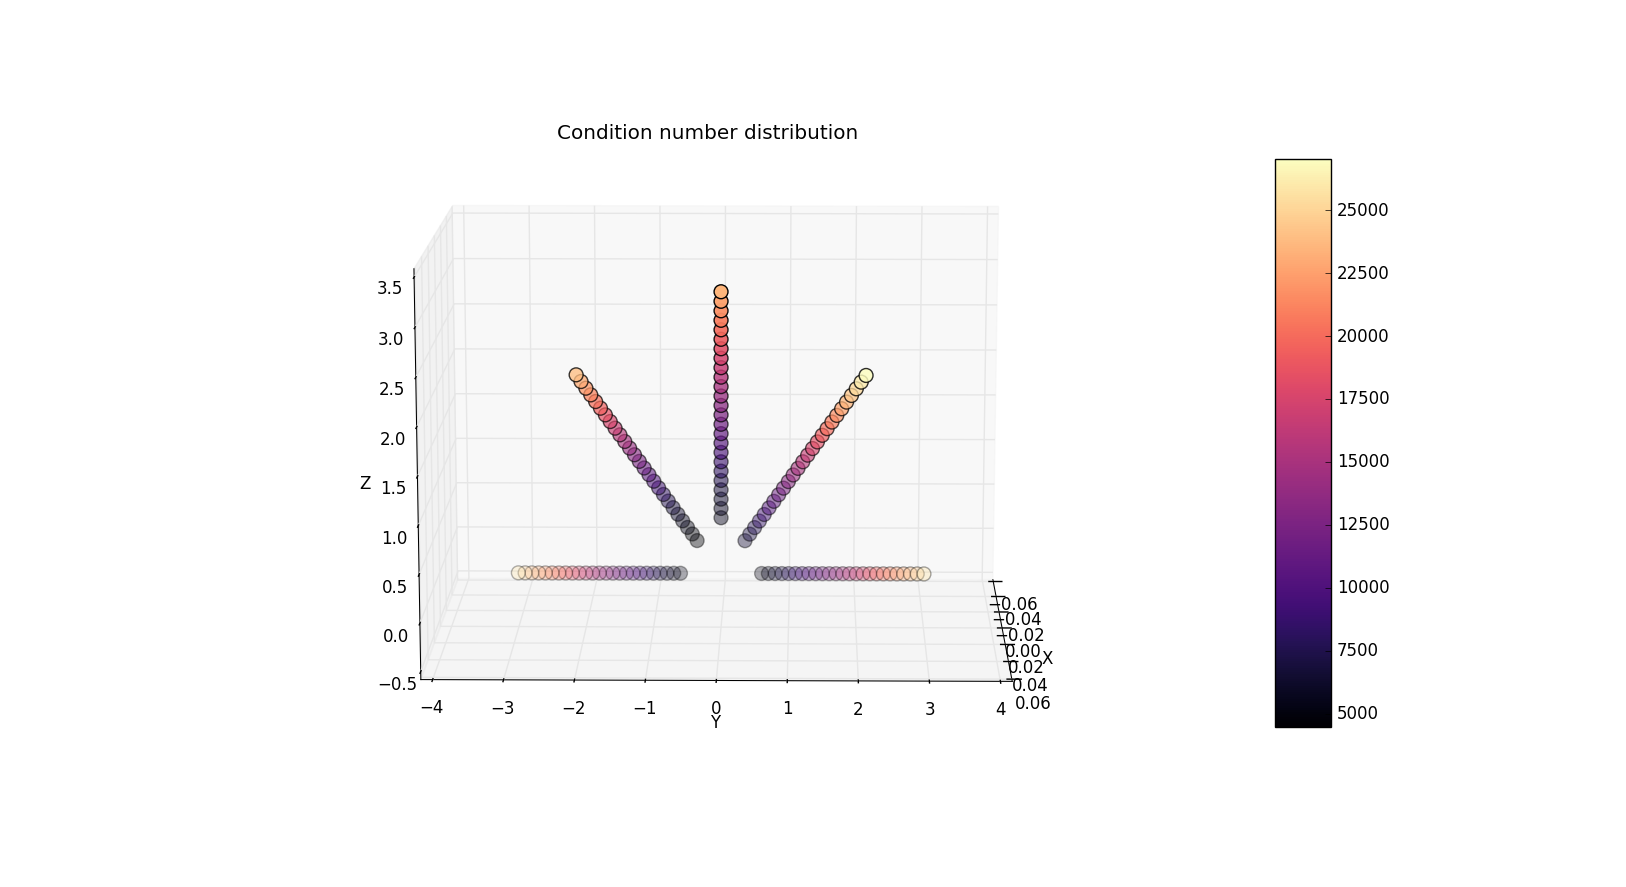
\includegraphics[width=\textwidth]{./fig/only_height.png}
    \caption{Influence of the height(distance between the cam1era and the marker) on the condition number of different camera positions while the angle is fixed as \SI{0}{\degree},\SI{45}{\degree},\SI{90}{\degree},\SI{135}{\degree} and \SI{180}{\degree}}
  \end{subfigure}
  \begin{subfigure}[b]{1.0\textwidth}
    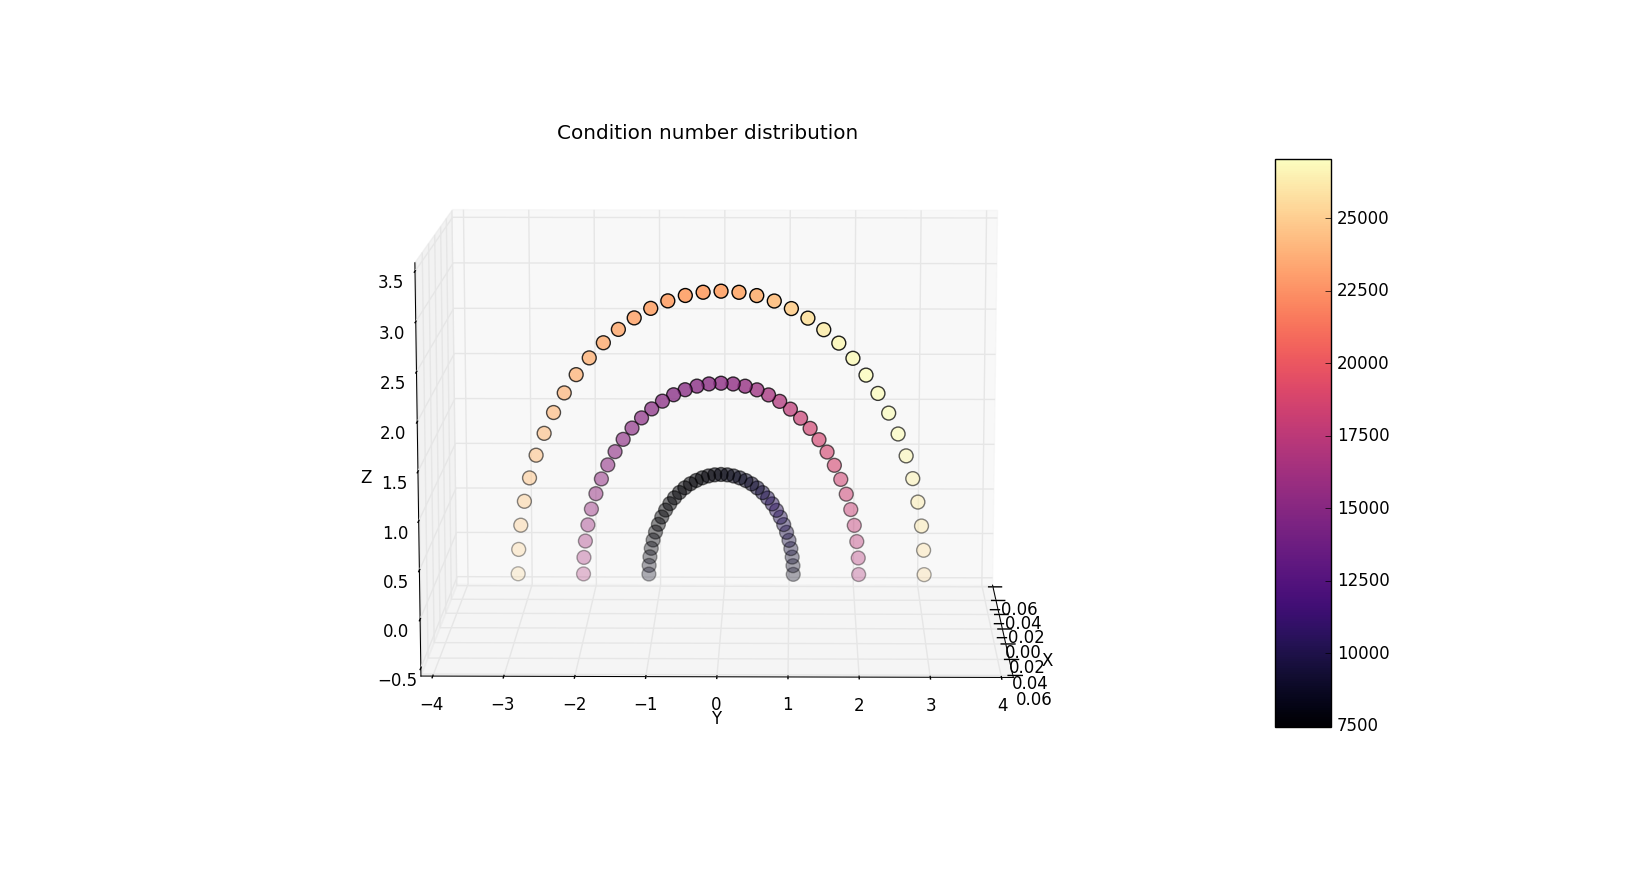
\includegraphics[width=\textwidth]{./fig/only_angle.png}
    \caption{Influence of the angle on the condition number of different camera positions while the height(distance between camera and marker) is fixed as 1.06666667m, 2.0333333 and 3m}
  \end{subfigure}
  \caption{Condition number distribution of different camera positions, each circle represents each camera position, different colors represent different values(figure \ref{fig:magma})}
  \label{fig:angle_height}
\end{figure}

\begin{figure}[H]
\hspace*{-4cm}
\centering
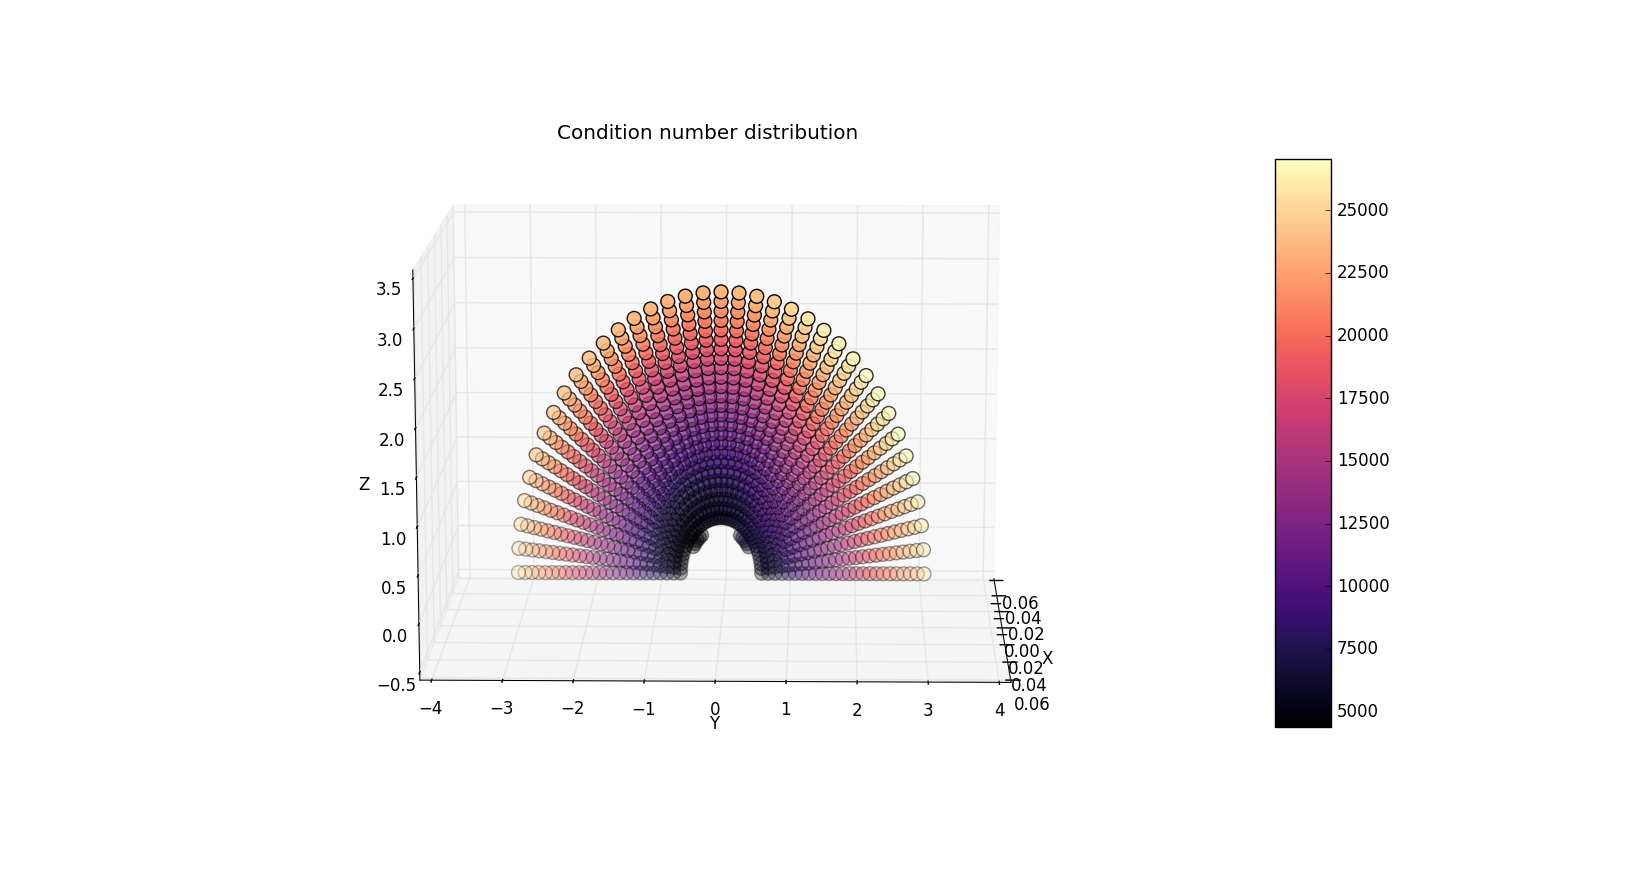
\includegraphics[scale=0.6]{./fig/cond_dis_noNor.png}
\caption{Condition number distribution(Interaction of \texttt{angle} and \texttt{height}), object points and image points are not normalized. The camera distribution is on YZ plane. The \texttt{angle} $\theta = [\SI{0}{\degree}, \SI{180}{\degree}]$, the step of angle is $\SI{5}{\degree}$, but in real world the angle can not be $\SI{0}{\degree}$ because of the constrain of DLT(three points that must be not collinear). The \texttt{height}(distance between camera and marker) as radius $ r= [0.1m, 3.0m]$, the step of radius is $0.1m$.}  
\label{fig:cond_dis_noNor}
\end{figure}

We can find that in figure \ref{fig:angle_height}(a) the condition number increases while the distance between camera and marker increases. This trend of condition number is consistent with previous results based on experiments in \cite{abawi2004accuracy} and \cite{pentenrieder2006analysis} and also is one of our desired result. 

However, in figure \ref{fig:angle_height}(b) it shows the condition number distribution is asymmetric. This is because that according to the equation mentioned in \cite{dynamic_markers}, we know that:
\begin{align*}
 c(A) = \norm{A}_2\norm{A^{-1}}_2 = \frac{s_{max}}{s_{min}}=\frac{s_1}{s_8}  
\end{align*}
and A is composed of four object points and four image points in our case,
we know that the object points are always set as constant(the coordinates in world coordinate system are fixed), so the only affected factor is related to the four image points. So we can see what is happened by image points:

Different camera position(Symmetrical cam position) on YZ plane has different rotation matrix \textbf{R}. And according to the corresponding rotation matrix \textbf{R} we can get different image points(camera model).

The symmetrical camera positions, which are closer to Z-axis ($\theta = 90$) and Y-axis ($\theta = 0$), get almost similar image points, similar image points lead to similar condition number. And the condition numbers on these symmetrical cam positions have smaller difference.
At somewhere $\theta$ between $0-90$, we get the biggest difference of condition number on symmetrical cam positions.

\begin{figure}[H]
\centering
\hspace*{-4cm}
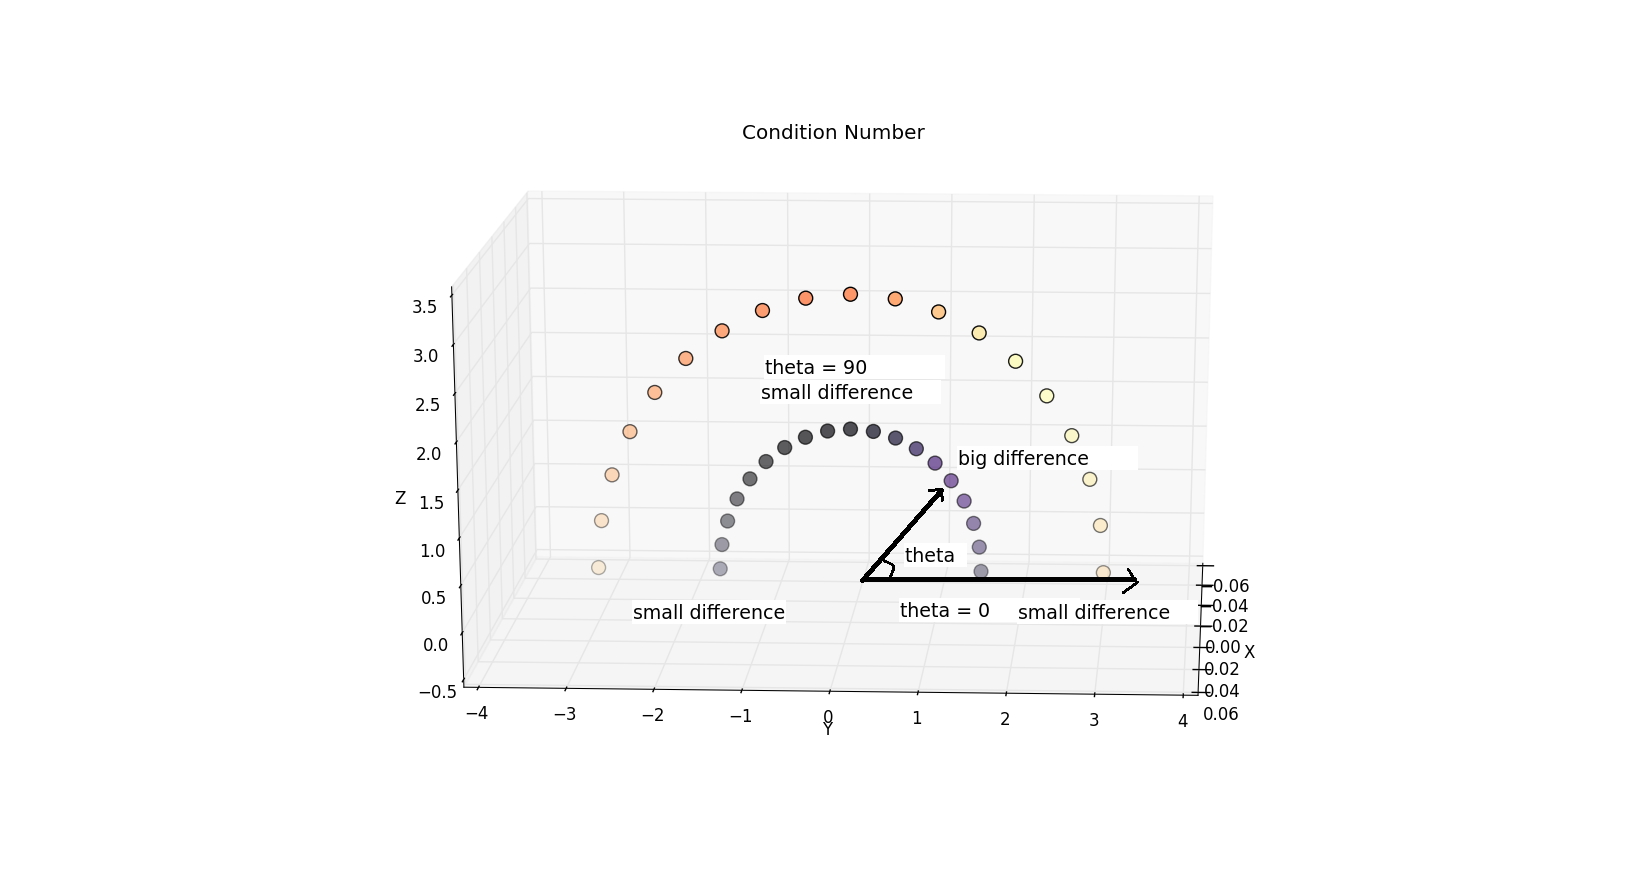
\includegraphics[scale=0.6]{./fig/connum_symm.png}
\caption{Symmetrical camera positions with different condition number}  
\label{fig:connum_symm}
\end{figure}

\begin{figure}[H]
  \centering
  \begin{subfigure}[b]{0.4\textwidth}
    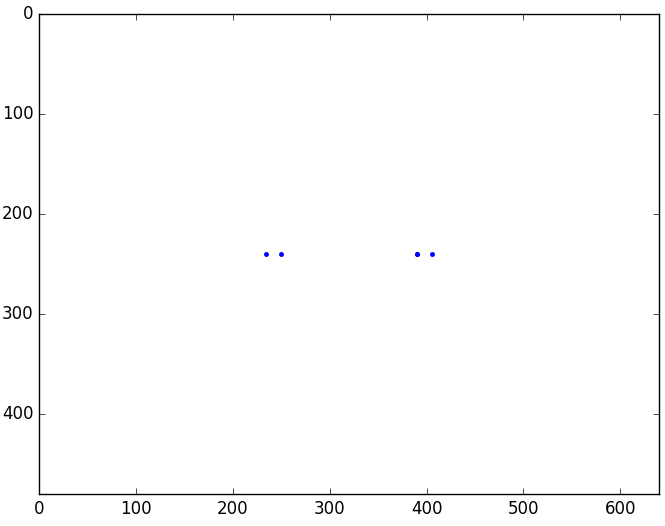
\includegraphics[width=\textwidth]{./fig/1.png}
    \caption{theta = $\SI{0}{\degree}$}
  \end{subfigure}
  \begin{subfigure}[b]{0.4\textwidth}
    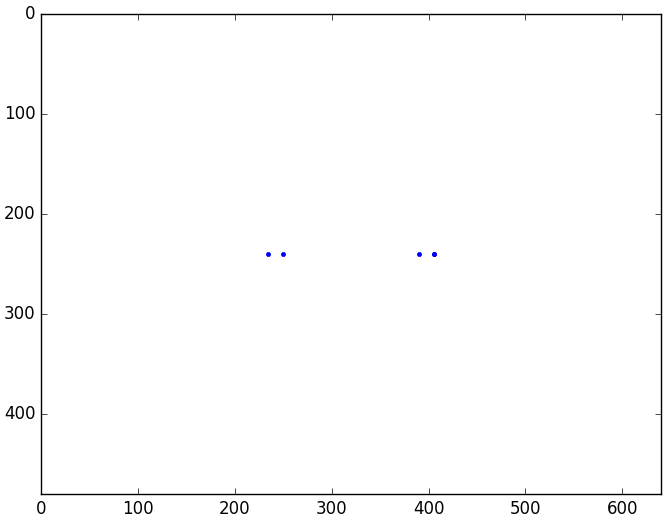
\includegraphics[width=\textwidth]{./fig/19.png}
    \caption{theta = $\SI{180}{\degree}$}
  \end{subfigure}
  
  \begin{subfigure}[b]{0.4\textwidth}
    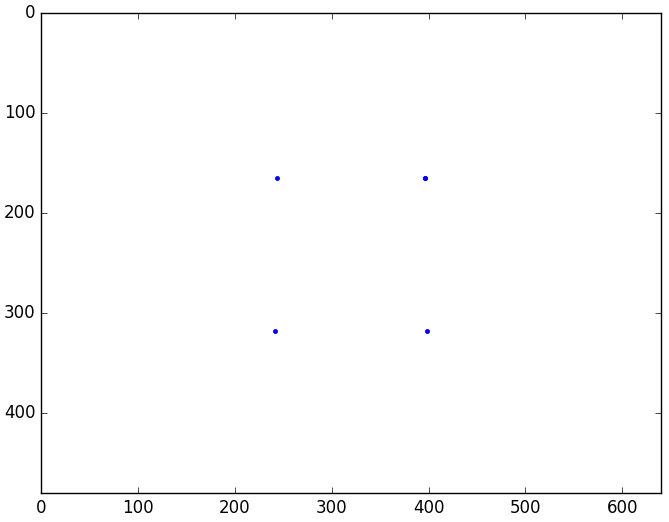
\includegraphics[width=\textwidth]{./fig/9.png}
    \caption{theta $\approx \SI{90}{\degree}, e.g. theta = \SI{89}{\degree}$}
  \end{subfigure}
  \begin{subfigure}[b]{0.4\textwidth}
    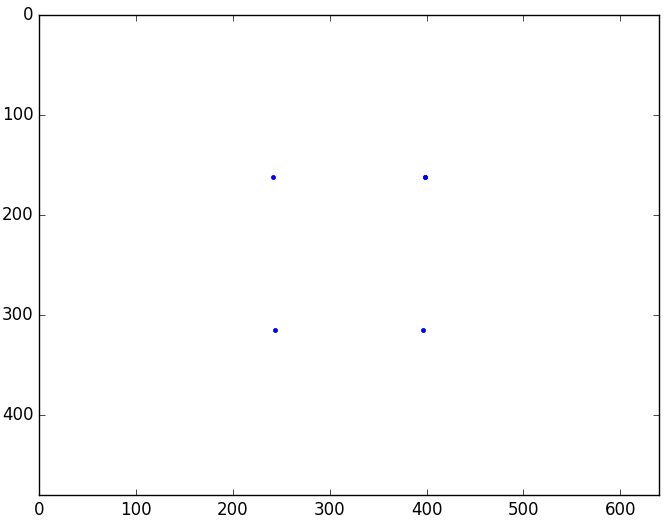
\includegraphics[width=\textwidth]{./fig/11.png}
    \caption{theta $\approx \SI{90}{\degree}, e.g. theta = \SI{91}{\degree}$}
  \end{subfigure}
    
    \begin{subfigure}[b]{0.4\textwidth}
    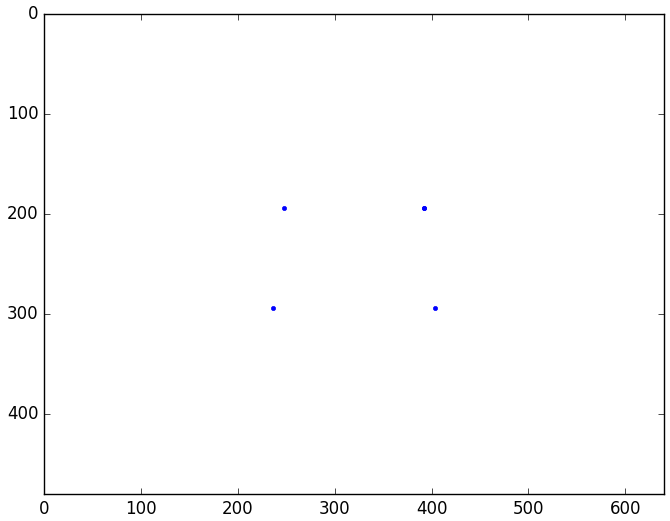
\includegraphics[width=\textwidth]{./fig/5.png}
    \caption{theta $\approx \SI{45}{\degree}$}
  \end{subfigure}
  \begin{subfigure}[b]{0.4\textwidth}
    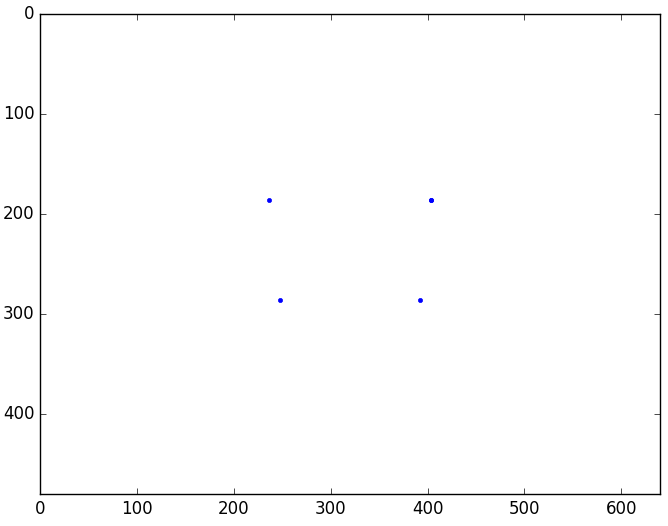
\includegraphics[width=\textwidth]{./fig/15.png}
    \caption{theta $\approx \SI{135}{\degree}$}
  \end{subfigure}
  \caption{When theta is equal to $\SI{0}{\degree}$ or $\SI{180}{\degree}$, image points exactly same. When theta closes to 90, image points exactly very similar. When theta closes to $\SI{45}{\degree}$ or $\SI{135}{\degree}$, image points have relative larger differences}
  \label{fig:119}
\end{figure}

In addition to asymmetric problem, there is another problem: 

The condition number is biggest when the angle of camera position is close to $\SI{90}{\degree}$, but this trend of condition number based on the change of angle is not a ideal and desired result. The reason for this problem is that without normalization of homography the differences of object points' order and image points' order are particularly large\cite{hartley2000multiple}. Therefore, we made regular normalization for both object points and image points in next step.\\

\texttt{Condition number distribution with normalized homography(regular normalization):}

We applied regular normalization for both object points and image points and made simulations under the same conditions as before.
 
\begin{python}\label{python:regular}
dist = []
pts = pts/pts[2, :]
for i in finiteind:
    c = np.mean(pts[0:2, i].T, axis=0).T
    newp1 = pts[0, i] - c[0]
    newp2 = pts[1, i] - c[1]
    dist.append(np.sqrt(newp1 ** 2 + newp2 ** 2))

dist = np.array(dist)
meandist = np.mean(dist)
scale = np.sqrt(2) / meandist # Translation and scaling
T = np.array([[scale, 0, -scale * c[0]], [0, scale, -scale * c[1]], [0, 0, 1]])
newpts = np.dot(T, pts)
return newpts,T
\end{python}

Figure \ref{fig:cond_dis_imageNor_angle_height} shows separately the condition number distribution in terms of \texttt{height} and \texttt{angle}, figure \ref{fig:cond_dis_imageNor} shows the condition number distribution at all positions.

\begin{figure}[H]
  \centering
  \begin{subfigure}[b]{1.0\textwidth}
    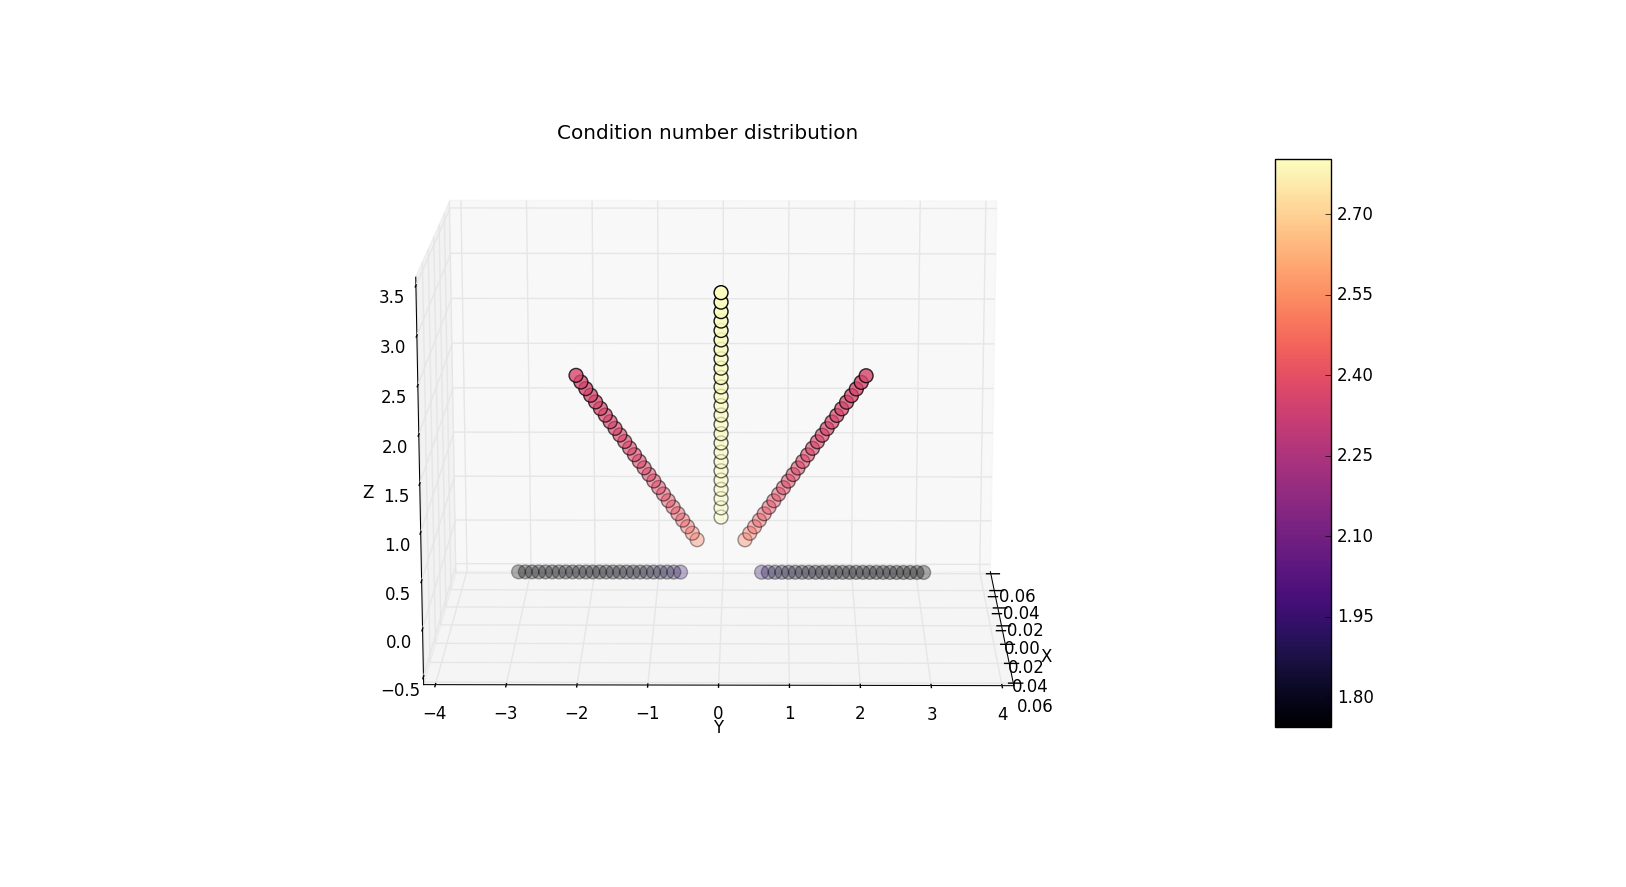
\includegraphics[width=\textwidth]{./fig/cond_dis_imageNor_height.png}
    \caption{Influence of the height(distance between the cam1era and the marker) on the condition number of different camera positions while the angle is fixed as \SI{0}{\degree},\SI{45}{\degree},\SI{90}{\degree},\SI{135}{\degree} and \SI{180}{\degree}}
  \end{subfigure}
  \begin{subfigure}[b]{1.0\textwidth}
    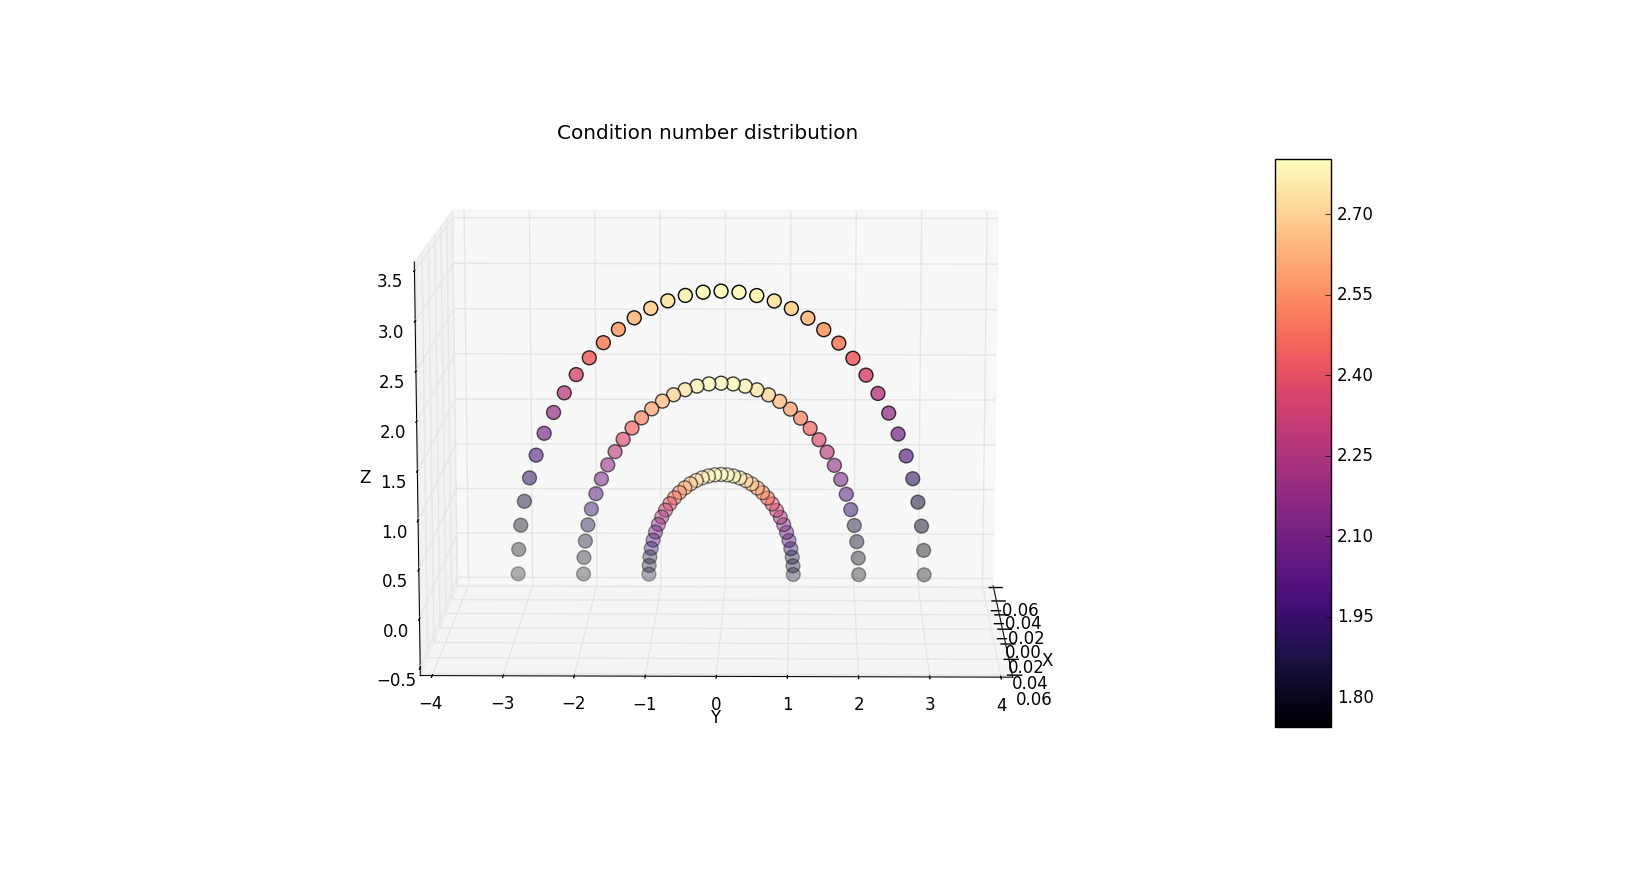
\includegraphics[width=\textwidth]{./fig/cond_dis_imageNor_angle.png}
    \caption{Influence of the angle on the condition number of different camera positions while the height(distance between camera and marker) is fixed as 1.06666667m, 2.0333333 and 3m}
  \end{subfigure}
  \caption{Condition number distribution of different camera positions, each circle represents each camera position, different colors represent different values(figure \ref{fig:magma})}
  \label{fig:cond_dis_imageNor_angle_height}
\end{figure}


\begin{figure}[H]
\hspace*{-4cm}
\centering
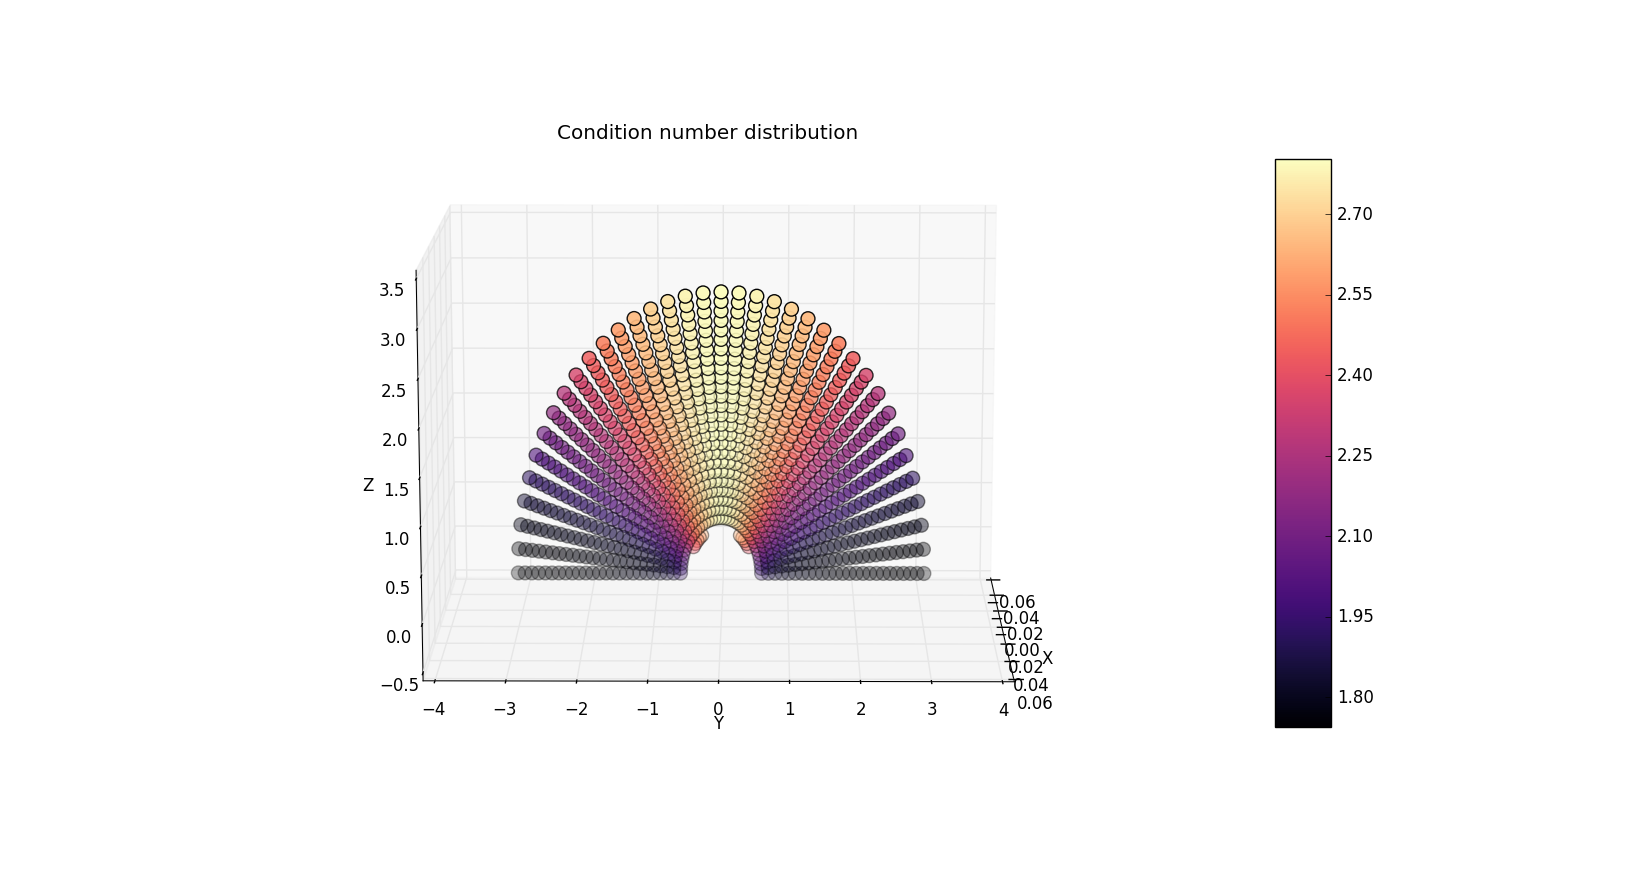
\includegraphics[scale=0.6]{./fig/cond_dis_imageNor.png}
\caption{Condition number distribution, object points and image points are both regular normalized}  
\label{fig:cond_dis_imageNor}
\end{figure}

From figure \ref{fig:cond_dis_imageNor_angle_height}(b) we can notice that this time the trend of condition number based on the change of the \texttt{angle} is our desired result, it is consistent with one of our desired results. However this time for each fixed angle shown in figure \ref{fig:cond_dis_imageNor_angle_height}(a) when the \texttt{height}(distance between camera and marker) increases, the condition number is still equal($angle = \SI{0}{\degree}$) or changed slightly($angle \neq \SI{0}{\degree}$). This is not a correct result.

The reason for this problem is that e.g. when the camera is set right above the marker($angle = \SI{0}{\degree}$) and moves directly above the marker, no matter where the camera is, the four image points in pixel coordinate system after normalization always locate at same positions. This leads to the equal condition number when the camera moves directly above the marker. This process is shown in figure \ref{fig:cam123} and figure \ref{fig:normalization}. Similarly, when the $angle \neq \SI{0}{\degree}$, the four image points in pixel coordinate system after normalization only change slightly, this leads to similar condition number.


\begin{figure}[H]
\centering
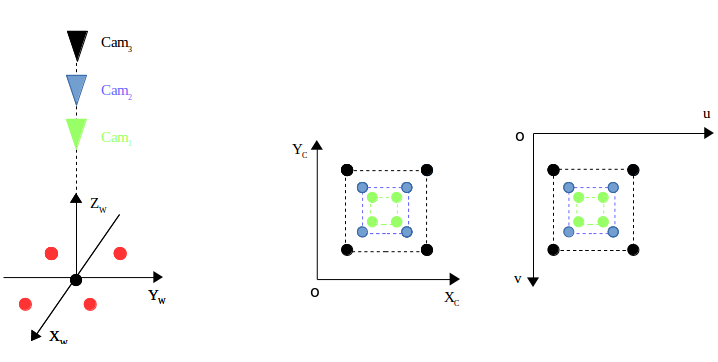
\includegraphics[scale=0.8]{./fig/cam123.png}
\caption{Test}  
\label{fig:cam123}
\end{figure}

\begin{figure}[H]
\centering
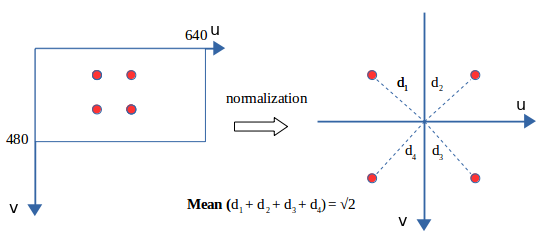
\includegraphics[scale=0.8]{./fig/normalization.png}
\caption{Normalization}  
\label{fig:normalization}
\end{figure}

\texttt{Condition number distribution with normalized homography(only translation but no scaling):}

We already know that we also need to consider the influence of the \texttt{height} on condition number. So we got one assumption: by normalization if we just implement the translation of the image points but not implement the scaling, maybe we we can get one ideal result. In order to verify this assumption we set the $scale = 1$ this times which means no scaling after translation of image points: 
\begin{python}\label{python:regular}
dist = []
pts = pts/pts[2, :]
for i in finiteind:
    c = np.mean(pts[0:2, i].T, axis=0).T
    newp1 = pts[0, i] - c[0]
    newp2 = pts[1, i] - c[1]
    dist.append(np.sqrt(newp1 ** 2 + newp2 ** 2))

dist = np.array(dist)
meandist = np.mean(dist)
scale = 1 # Only translation, no scaling
T = np.array([[scale, 0, -scale * c[0]], [0, scale, -scale * c[1]], [0, 0, 1]])
newpts = np.dot(T, pts)
return newpts,T
\end{python}

But obviously we got the result still with problem which is shown in figure \ref{fig:con_dis_Imag_OnlyTrans}. This figure shows that when the camera is closer to the marker, the condition number gets bigger. It is exactly the opposite of what we want.

The reason for this problem is that if the camera locates closer to the marker, the closer the four image points are to the origin of pixel coordinate. And according to the matrix \texttt{A} of condition number, if the image points locate closer to the origin of pixel coordinate, the smaller the condition number is. Therefore in this case we got a opposite conclusion.

\begin{figure}[H]
\hspace*{-4cm}
\centering
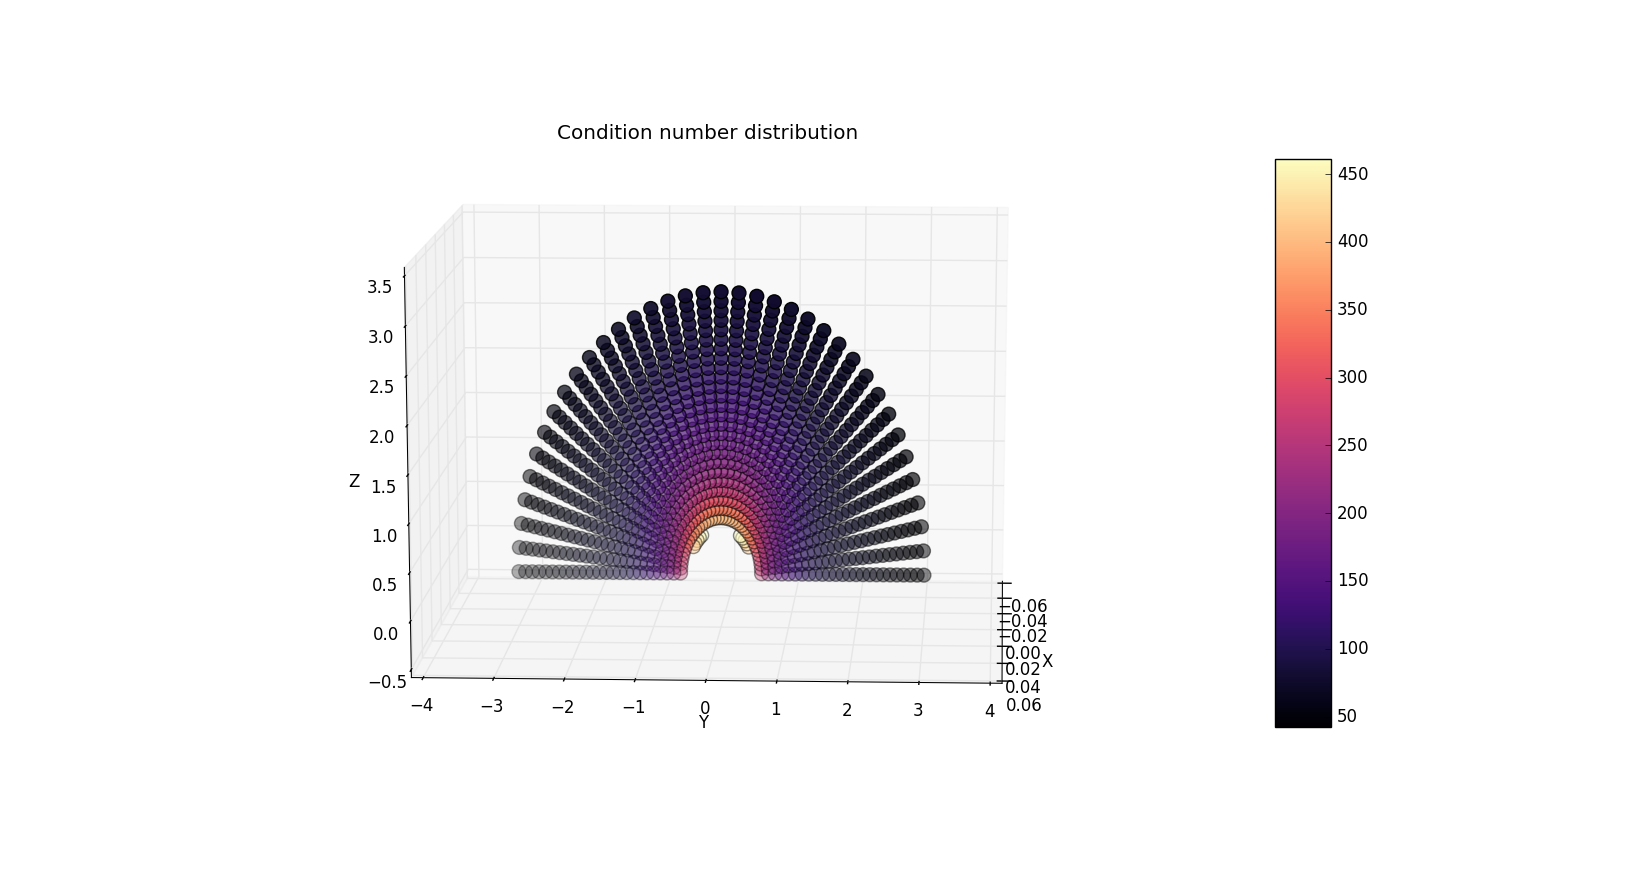
\includegraphics[scale=0.6]{./fig/con_dis_Imag_OnlyTrans.png}
\caption{Condition number distribution, object points are regular normalized and image points are normalized only with translation but no scaling(scale = 1)}  
\label{fig:con_dis_Imag_OnlyTrans}
\end{figure}

If in this case we got a opposite conclusion, can we just make a little trick that we set condition number as it's reciprocal?
\begin{python}\label{python:regular}
mat_cond = gd.matrix_condition_number_autograd(*input_list, normalize = normalized)
# TODO normalized with no scaling (scale = 1) , invert the condtion number
mat_cond = 1 / mat_cond
\end{python}

After performing this little trick, we found that the trend of condition number in terms of the change of \texttt{angle} is still not right, which is shown in figure \ref{fig:angleHeight_invert_condNum}(b). The reason is that before we applied the reciprocal of condition number, when the height is fixed, it has a lower condition number if the angle is smaller. Therefore when we applied the reciprocal of condition number, the lower angle has a bigger condition number.

\begin{figure}[H]
  \centering
  \begin{subfigure}[b]{1.0\textwidth}
    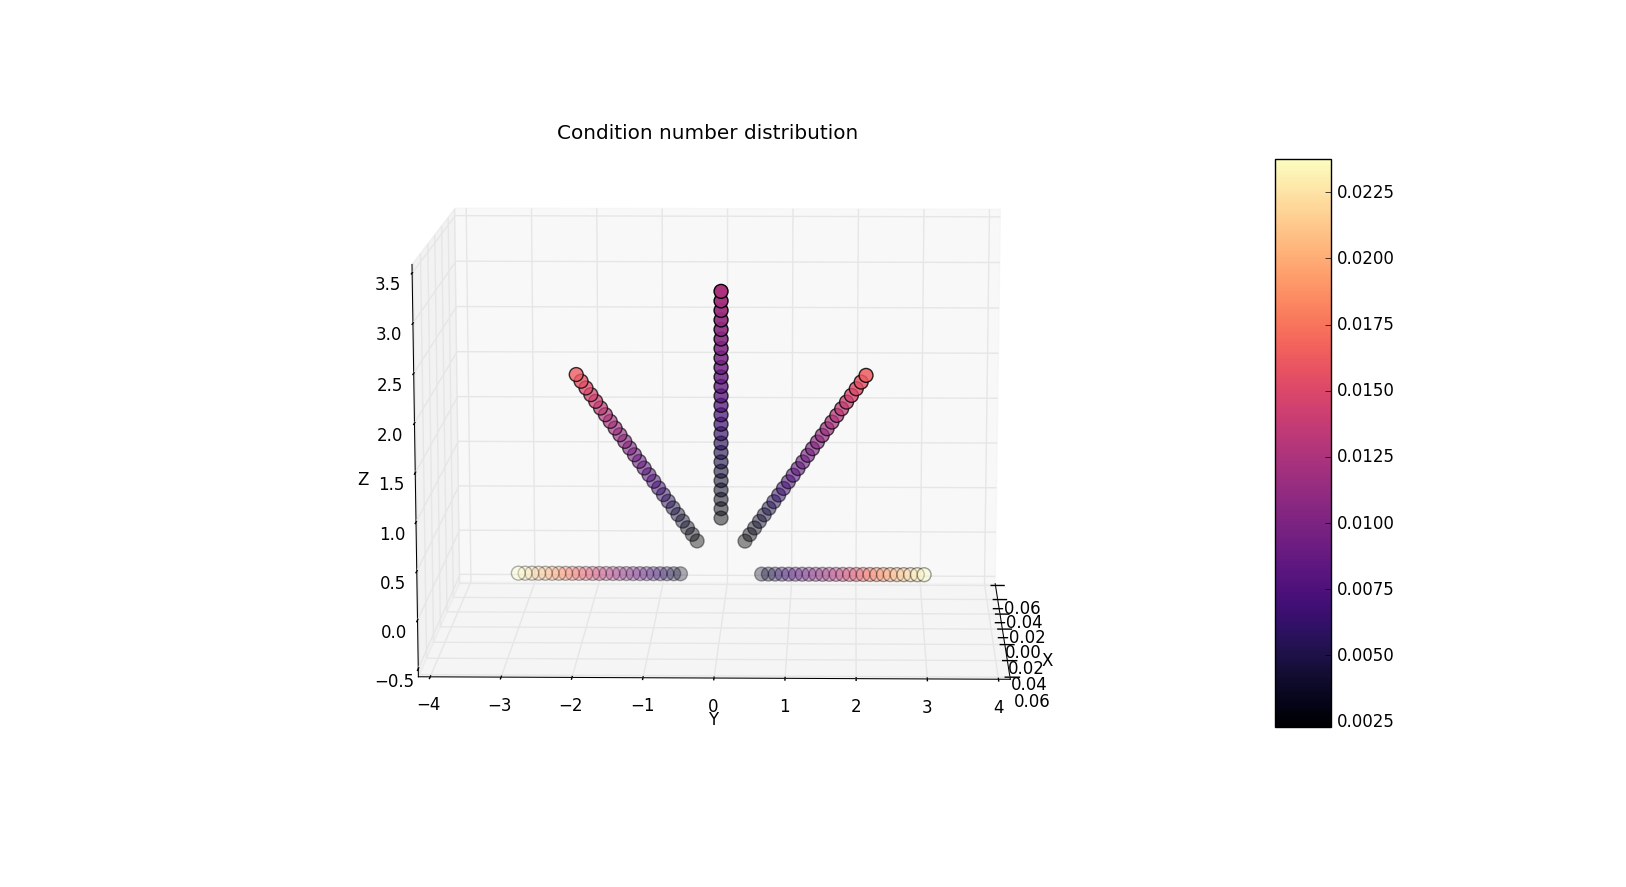
\includegraphics[width=\textwidth]{./fig/cond_num_dis_height.png}
    \caption{Condition number distribution when the angle is fixed as \SI{0}{\degree},\SI{45}{\degree},\SI{90}{\degree},\SI{135}{\degree} and \SI{180}{\degree}($condition number = 1/condition number $ }
  \end{subfigure}
  \begin{subfigure}[b]{1.0\textwidth}
    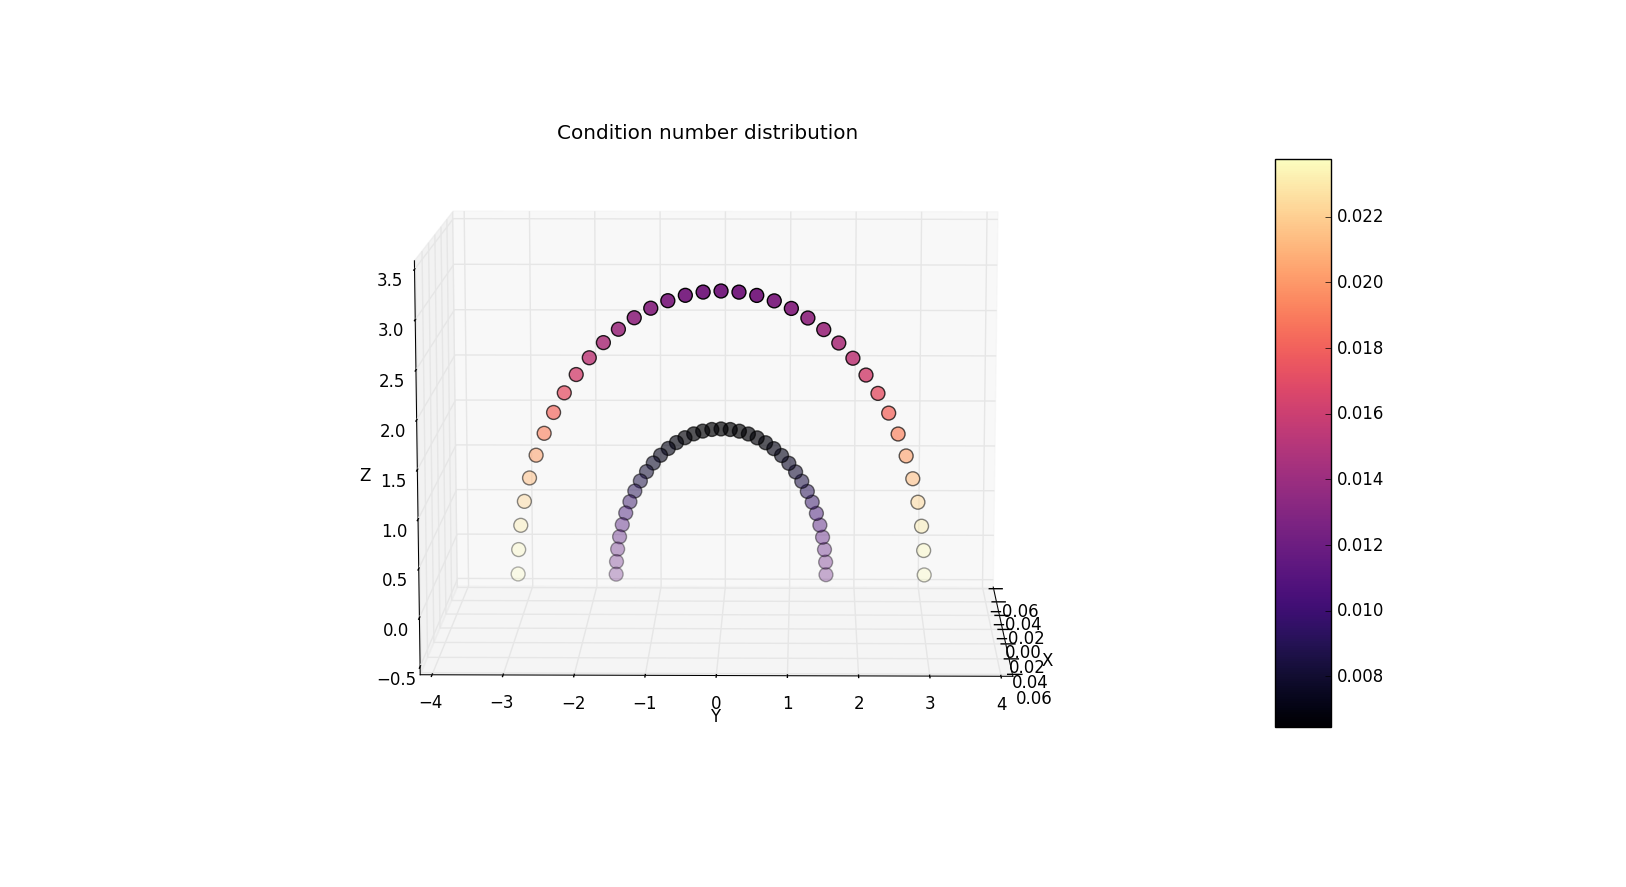
\includegraphics[width=\textwidth]{./fig/angle_invert_condNum.png}
    \caption{Condition number distribution when the height fixed at 1.55m and 3m($condition number = 1/condition number $}
  \end{subfigure}
  \caption{Condition number distribution of different camera positions, each circle represents each camera position, different colors represent different values(figure \ref{fig:magma})}
  \label{fig:angleHeight_invert_condNum}
\end{figure}  
  
\begin{figure}[H]
\hspace*{-4cm}
\centering
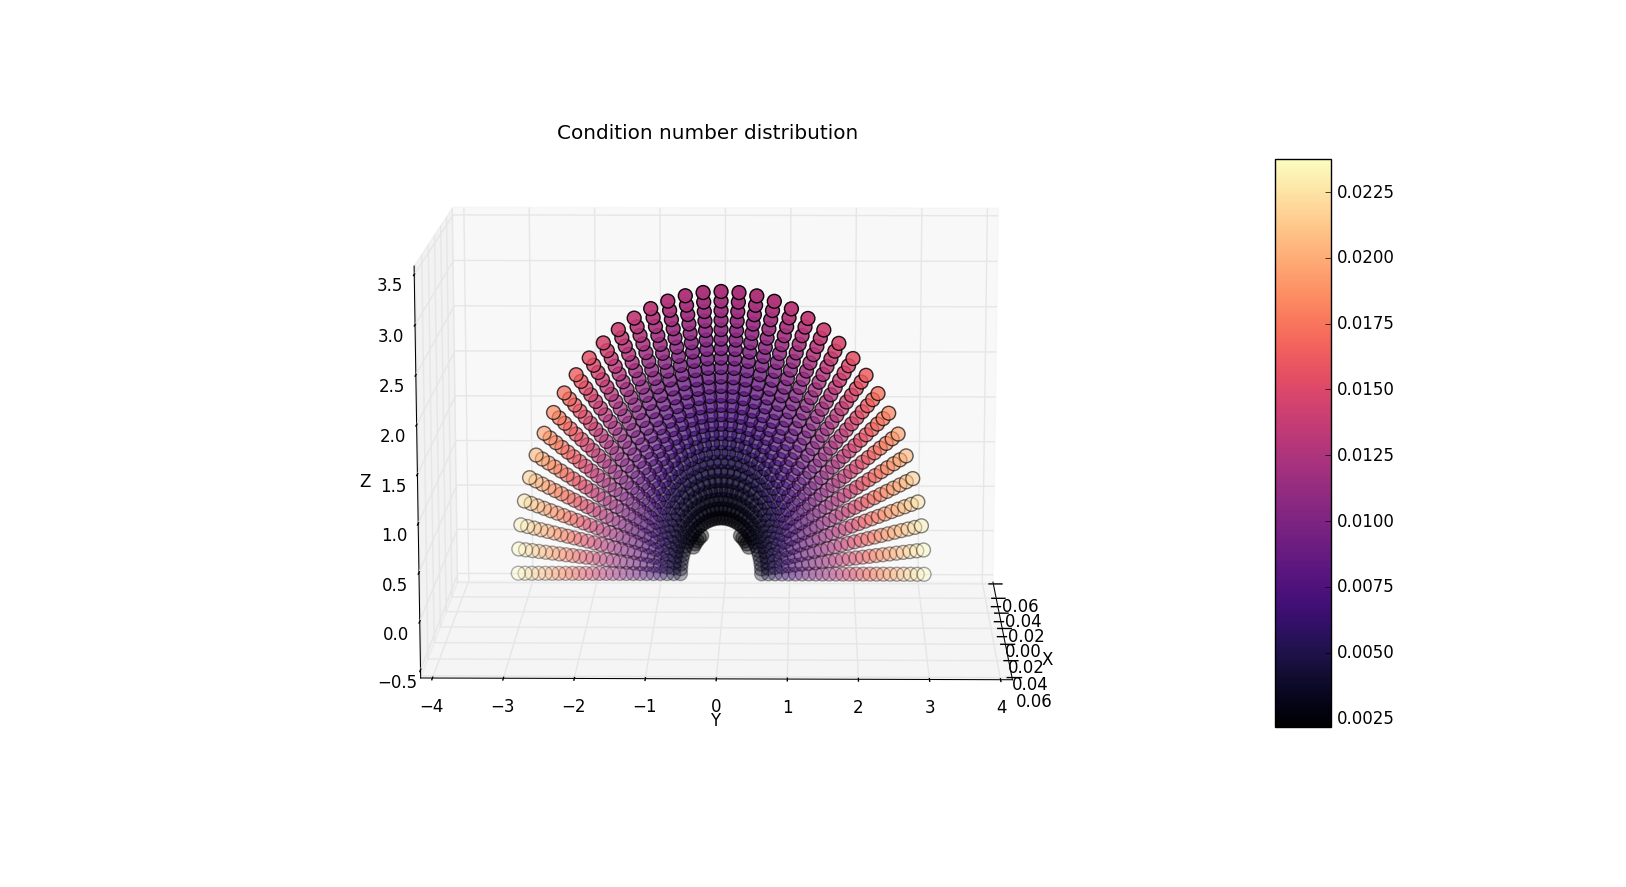
\includegraphics[scale=0.6]{./fig/invert_condNum.png}
\caption{Condition number distribution, object points are regular normalized and image points are normalized only with translation but no scaling(scale = 1), but $condition number = 1/condition number $}  
\label{fig:invert_condNum}
\end{figure}

\texttt{Condition number distribution with normalized homography(scale based on height):}

After all of these simulations, we used another trick: we set the product of height and regular normalized scale as the new scale of normalization:

\begin{python}\label{python:regular}
dist = []
pts = pts/pts[2, :]
for i in finiteind:
    c = np.mean(pts[0:2, i].T, axis=0).T
    newp1 = pts[0, i] - c[0]
    newp2 = pts[1, i] - c[1]
    dist.append(np.sqrt(newp1 ** 2 + newp2 ** 2))

dist = np.array(dist)
meandist = np.mean(dist)
scale = radius*np.sqrt(2)/meandist # Set the scale increasing with distance from camera to marker
T = np.array([[scale, 0, -scale * c[0]], [0, scale, -scale * c[1]], [0, 0, 1]])
newpts = np.dot(T, pts)
return newpts,T
\end{python}

And we got following desired results which are shown in figure \ref{fig:cond_num_Imag_Rnor_angleHeight}, this condition number distribution computed with this approach can be interpreted as the accuracy function.

\begin{figure}[H]
  \centering
  \begin{subfigure}[b]{1.0\textwidth}
    \includegraphics[width=\textwidth]{./fig/cond_num_Imag_Rnor_height.png}
    \caption{Condition number distribution, object points are regular normalized and image points are normalized with $scale = radius*np.sqrt(2) / meandist$. The angle is fixed as \SI{0}{\degree},\SI{45}{\degree},\SI{90}{\degree},\SI{135}{\degree} and \SI{180}{\degree}}
  \end{subfigure}
  \begin{subfigure}[b]{1.0\textwidth}
    \includegraphics[width=\textwidth]{./fig/cond_num_Imag_Rnor_angle.png}
    \caption{Condition number distribution, object points are regular normalized and image points are normalized with $scale = radius*np.sqrt(2) / meandist$. The height is fixed as 1.06666667m, 2.0333333 and 3m}
  \end{subfigure}
  \caption{Condition number distribution of different camera positions, each circle represents each camera position, different colors represent different values(figure \ref{fig:magma})}
  \label{fig:cond_num_Imag_Rnor_angleHeight}
\end{figure}  

\begin{figure}[H]
\hspace*{-4cm}
\centering
\includegraphics[scale=0.6]{./fig/cond_num_Imag_Rnor.png}
\caption{Condition number distribution, object points are regular normalized and image points are normalized with $scale = radius*np.sqrt(2) / meandist$}  
\label{fig:cond_num_Imag_Rnor}
\end{figure}

The figure \ref{fig:cond_num_Imag_Rnor_angleHeight}(a) shows the trend of condition number based on the change of \texttt{h}. We can find that when the camera is close to the origin of marker, it has a relative small condition number at this corresponding position. This is consistent with one of our desired results.

The figure \ref{fig:cond_num_Imag_Rnor_angleHeight}(b) shows the trend of condition number based on the change of \texttt{angle}. We can find that when the camera is close to the x-axis, it has a relative small condition number at this corresponding position. And the condition number distribution is exactly symmetrical. This is also consistent with another one of our desired results.\\

\texttt{Results summary:}

There is no doubt that normalization of homopraphy is an essential step to compute condition number of different camera positions for the accuracy function. However how to implement the meaningful normalization(e.g. how should the coordinates should be scaled?) is one step worth to think about.
 
After many simulations and considering different cases, we used one little trick to compute our desired condition number: we chose to scale the coordinates: the average distance of
a point x from the origin is equal to $radius \times \sqrt{2}$.

Using this little trick we got our desired results mentioned at the beginning of this section: 
The closer the camera is to the marker, the smaller the condition number is which means the more accurate the camera pose. However in the real case in view of the camera's detection range the camera can not be placed too close to the marker and the angle between the camera and the marker plane can not be too small. We can treat the condition number distribution as our accuracy function. Our results about condition number distribution were similar to the accuracy as a function of camera distance and relative camera angle in \cite{abawi2004accuracy} and \cite{pentenrieder2006analysis}.
\chapter{Accuracy of Monocular Tracking using Error Covariance Matrix}
\label{chap:Accuracy of Monocular Tracking using Error Covariance Matrix}

In \cite{bauer2007tracking}
an approach using error covariance matrix to represent the accuracy of monocular tracking is introduced. However this approach does not apply to our situation and I regard the method mentioned in this paper with suspicion. In this section I will explain in detail why this method does not work for our situation.

\section{Gaussian error distributions}

\subsection{Multi-dimensional Gaussian distributions}
\textbf{Gaussian distribution} is a very common continuous probability distribution. In our project we also set the image noisy(errors) as Gaussian distribution. We directly focus on the \textit{n}-dimensional Gaussian distribution which is shown in figure \ref{fig:gaussian}, the form of corresponding probability density function is:

\begin{align}\label{eq:cee1}
 f_{\mu,\Sigma}(x)= \frac{1}{\sqrt{( 2\pi)^n|\Sigma|}}exp^{\big(-\frac{1}{2}(x - \mu)^T \Sigma^{-1} (x - \mu) \big)}
\end{align}
where $\mu \in \mathbb{R}^n$ denotes the mean of random variable vector and $\Sigma \in \mathbb{R}^{n \times n}$ covariance matrix.

\begin{figure}[h!]
\centering
\includegraphics[scale=0.5]{./fig/gaussian.png}
\caption{Probability density function of 2 dimensional Gaussian distribution}  
\label{fig:gaussian}
\end{figure}

A \textit{n}-dimensional covariance matrix $\boldsymbol{\Sigma}$ is always symmetric and positive semi-definite, which means the eigenvalues of covariance matrix are non-negative.

\begin{align*}
\Sigma =   \begin{bmatrix} var(x1) & cov(x_1,x_2) & \cdots & cov(x_1,x_n) \\
                 cov(x_1,x_2) & var(x2) & \cdots & cov(x_n,x_2) \\
                 \vdots  & \vdots  & \ddots & \vdots  \\
                 cov(x_1,x_n) & cov(x_2,x_n) & \cdots & var(x_n) \\ \end{bmatrix} 
\end{align*}

\subsection{Confidence ellipse/ellipsoid}
The confidence ellipse which is also known as error ellipse represents an isocontour of the two dimensional Gaussian distribution and allow you to visualize the selected confidence level. In contrast to confidence ellipse, the confidence ellipsoid represents a visualization of three dimensional Gaussian distribution. 

Now we make a derivation from the probability function(equation \ref{eq:cee1}) and assume that the mean $\mu$ of random variable is zero:
\begin{align*}
p &= \frac{1}{\sqrt{( 2\pi)^n|\Sigma|}}exp^{\big(-\frac{1}{2}(x - \mu)^T \Sigma^{-1} (x - \mu) \big)}\\
\Downarrow \\
p \sqrt{( 2\pi)^n|\Sigma|} &= exp^{\big(-\frac{1}{2}(x - \mu)^T \Sigma^{-1} (x - \mu) \big)}\\
\Downarrow \\
(x - \mu)^T \Sigma^{-1} (x - \mu) &= -2 \ln{p \sqrt{( 2\pi)^n|\Sigma|}}\\
\Downarrow \\
x^T \Sigma^{-1} x &= -2 \ln{p \sqrt{( 2\pi)^n|\Sigma|}} = s
\end{align*}

In general, we can use following equations to describe ellipse and ellipsoid:

\begin{align*}
(\frac{x}{a})^2 + (\frac{y}{b})^2 &= 1 & \text{a,b: length of semi-major axis and length of semi-minor axis}\\
(\frac{x}{a})^2 + (\frac{y}{b})^2 + (\frac{z}{c})^2 &= 1 & \text{a,b,c: semi-axes}
\end{align*}

From covariance matrix we can derive the forms similar to the above equations:

\begin{align*}
\frac{x^2}{\lambda_x} + \frac{y^2}{\lambda_y} &= s \\
\frac{x^2}{\lambda_x} + \frac{y^2}{\lambda_y} + \frac{z^2}{\lambda_z} &= s
\end{align*}
where $\lambda_x$, $\lambda_y$ and $\lambda_z$ are the eigenvalues of the corresponding covariance matrix, \textit{s} defines the scale of the ellipse which could be any arbitrary number. Then we turn the question into how to find \textit{s}, in our case we use confidence level to represent the scale \textit{s}. The relationship between confidence level and scale \textit{s} for different dimensions is shown in table \ref{table:confidence_level}.

\begin{table}[h]
\begin{tabular}{ |l|l|l|l|l|l|l| }
\hline
\multicolumn{7}{ |c| }{Confidence Level} \\
\hline
Dimension & 25\% & 50\% & 75\% & 95\% & 97\% & 99\% \\ \hline
n = 1 & 0.10153  & 0.45494 & 1.3233 & 3.84146 & 4.70929 &  6.6349\\
n = 2 & 0.57536  & 1.38629 & 2.77259 & 5.99146 & 7.01312 &  9.2103 \\
n = 3 & 1.21253  & 2.36597 & 4.10834 & 7.81473 & 8.94729 &  11.3449 \\
\hline
\end{tabular}
\caption[Table caption text]{The value of scale \textit{s} in different confidence levels for different dimensions. e.g. if n = 2 and confidence level is 95\% then the scale \textit{s} is 5.99146\cite{bauer2007tracking}}
\label{table:confidence_level}
\end{table}

Now we make a transform of ellipse and ellipsoid, multiply $\frac{1}{s}$ on both sides of equations:
\begin{align*}
(\frac{x}{ \sqrt{s\lambda_x}})^2 + (\frac{y}{\sqrt{s\lambda_y }})^2 &= 1 \\
(\frac{x}{\sqrt{s\lambda_x }})^2 + (\frac{y}{\sqrt{s\lambda_y }})^2 + (\frac{z}{\sqrt{s\lambda_z }})^2 &= 1
\end{align*}

we find that the length of the axes of ellipse or ellipsoid can be represented as $l_i = \sqrt{s\lambda_i}(i = 1,2,3)$. We can use this formula to calculate the length of axes and then plot the covariance ellipse or ellipsoid for a certain confidence level as an example shown in figure \ref{fig:confidence2D} and figure \ref{fig:ellipsoid}.

\begin{figure}[h!]
\centering
\includegraphics[width=0.9\textwidth]{./fig/confidence2D.png}
\caption{Confidence ellipses for normally distributed data with different confidence levels\cite{vincent_spruyt}} 
\label{fig:confidence2D}
\end{figure}


\begin{figure}[h!]
\centering
\includegraphics[width=0.9\textwidth]{./fig/ellipsoid.png}
    \caption{Visualization of covariance ellipsoid for a certain confidence level\cite{bauer2007tracking}}
\label{fig:ellipsoid}
\end{figure}

\section{Error propagation for Gaussian distributions} 
Two propagation methods are introduced in ...%
which are used to describe Gaussian errors propagation in linear or non-linear functions of monocular tracking system.
\section{Forward propagation} 
For the linear function, if the random variable $\textit{v}$ is a Gaussian distribution then the linear function $f(v)$ is also a Gaussian distribution. We assume that the linear function is describe as $f(v) = Av$, the mean of variable $\textit{v}$ is $\overline{v}$ and the covariance matrix is $\Sigma$. Then the linear function $f(v)$ is also a random variable with mean $f(\overline{v})$ and covariance matrix $\Sigma_f$. This relationship is shown in table \ref{table:linear_function}:

\begin{table}[h!]
\begin{center}
\begin{tabular}{ |l|l|l| }
\hline
 & mean & covariance matrix \\ \hline
$v$ & $\overline{v}$  & $\Sigma$ \\
$f(v)$ & $f(\overline{v})$ & $\Sigma_f = A \Sigma A^T$ \\
\hline
\end{tabular}
\caption[Table caption text]{Linear function: $f(v) = Av $}
\label{table:linear_function}
\end{center}
\end{table}

For the non-linear function $f(v)$, in order to apply the Gaussian distribution forward propagation we need to build an approximation of the non-linear function. We can use Taylor expansion to  present the first order approximation:

\begin{align*}
f(v) = f(v_0 + \Delta_v) = f(v_0) + J_f(v_0)\Delta_v + \mathcal{O}{v^2}
\end{align*}

For the non-linear function $f(v)$ we assume that the mean of variable $\textit{v}$ is $\overline{v}$ and the covariance matrix is $\Sigma$. Then the non-linear function $f(v)$ is a random variable with mean $f(\overline{v})$ and covariance matrix $\Sigma_f$. This relationship is shown in table \ref{table:nonlinear_function}:

\begin{table}[h!]
\begin{center}
\begin{tabular}{ |l|l|l| }
\hline
 & mean & covariance matrix \\ \hline
$v$ & $\overline{v}$  & $\Sigma$ \\
$f(v)$ & $f(\overline{v})$ & $\Sigma_f = J_f \Sigma J_f^T$ \\
\hline
\end{tabular}
\caption[Table caption text]{Non-linear function: $f(v)$}
\label{table:nonlinear_function}
\end{center}
\end{table}

where $J_f$ is the Jacobian matrix of non-linear function $f(v)$ evaluated at $\overline{v}$.

\section{Backward propagation} 

In some situation if the covariance matrix $\Sigma_f$ of function $f(v)$ is given and we want to know the covariance $\Sigma$ of the variable \textit{v}. We can use the following equation to compute the backward propagation:

\begin{align*}
\Sigma = (J_f^T \Sigma_f^{-1} J_f)^{-1}
\end{align*}

where $J_f$ is the Jacobian matrix of non-linear function $f(v)$ evaluated at $\overline{v}$.
This backward propagation is the main idea to compute the accuracy of monocular tracing in \cite{bauer2007tracking}

\section{Accuracy of monocular tracking}
In \cite{bauer2007tracking}
the computation of accuracy of monocular tracking is under a theoretical model, which the topology of the target is known exactly and all the features from the target can be well recognized and that the 2D position estimation is unbiased but not noise free. In \cite{bauer2007tracking}
a spherical coordinate system is used to represent the pose of camera in world.

\begin{figure}[h!]
\centering
\includegraphics[width=0.5\textwidth]{./fig/spherical.png}
    \caption{Setup for analyzing the theoretical accuracy of a monocular tracking
system with planar fiducials\cite{bauer2007tracking}}
\label{fig:spherical}
\end{figure}

In this case the camera pose can be described with 3 parameters($\alpha,\beta,r$) instead of six-dimensional pose($x,y,z,\alpha,\beta,\gamma$), so a covariance matrix $\Sigma_{\alpha,\beta,r} \in \mathbb{R}^{n \times n}$ can represent the error for each camera position.

Recall that the pinhole camera model, the relationship between world coordinate system and pixel coordinate system.
\begin{equation}\label{eq:zckt}
Z_C \begin{bmatrix} u \\ v \\ 1 \end{bmatrix}
      = KT                                         
        \begin{bmatrix} X_W \\ Y_W \\ Z_W \\ 1 \end{bmatrix}                 
\end{equation}
where camera intrinsic parameters \textbf{K} is constant and in our situation we set it as:
\begin{equation*}
K =  \begin{bmatrix} 800 & 0 & 320 \\ 0 & 800 & 240 \\ 0 & 0 & 1\end{bmatrix}                 
\end{equation*}
According to \cite{bauer2007tracking}
without loss of generality the camera extrinsic parameters \textbf{T}([\textbf{R}$|$\textbf{t}]) can be parametrized with $\alpha,\beta,\gamma$ and the following equations show how to get the rotation matrix \textbf{R} based on coordinate transformation, this process is shown in figure \ref{fig:NAB}.
\begin{align*}\label{eq:nrb}
\tensor*[^N]{R}{^B} &= \tensor*[^N]{R}{^A} \cdot \tensor*[^A]{R}{^B}\\
               &=\begin{bmatrix} 
                cos(\alpha)cos(\beta) & -sin(\beta) & sin(\alpha)cos(\beta) \\
                cos(\alpha)sin(\beta) & cos(\beta) & sin(\alpha)sin(\beta)  \\
                sin(\alpha) & 0 & cos(\alpha)
                \end{bmatrix} 
\end{align*}
Because the positive direction of the camera \textit{z}-axis always points to the origin where the marker is placed in the world coordinate system, the rotation matrix $\tensor*[^N]{R}{^B}$ still needs to rotate $\SI{180}{\degree}$ around \textit{x}-axis:
\begin{align*}
R = R_x(\pi) \cdot \tensor*[^N]{R}{^B}\\
\end{align*}

\begin{figure}[h!]
\centering
\includegraphics[width=0.5\textwidth]{./fig/NAB.png}
    \caption{Rotation in spherical coordinate system}
\label{fig:NAB}
\end{figure}

And from Cartesian coordinates to spherical coordinates transformation we know that the translation vector \textbf{t} can be presented using there parameters $\alpha,\beta,\gamma$ as:
\begin{align*}
x &= r \cdot cos(\beta) \cdot sin(\alpha) \\
y &= r \cdot sin(\beta) \cdot sin(\alpha)\\
z &= r \cdot cos(\alpha)
\end{align*}
Now the camera extrinsic parameters \textbf{T}([\textbf{R}$|$\textbf{t}]) can be presented as:
\begin{align*}
T &=\begin{bmatrix} 
                cos(\alpha)cos(\beta) & -sin(\beta) & sin(\alpha)cos(\beta) & r cos(\beta) sin(\alpha)\\
                cos(\alpha)sin(\beta) & cos(\beta) & sin(\alpha)sin(\beta)  & r sin(\beta) sin(\alpha)\\
                sin(\alpha) & 0 & cos(\alpha) & r cos(\alpha) \\
                0 & 0 & 0 & 1                
                \end{bmatrix} 
\end{align*}
Because we already know the expression of the camera extrinsic parameters \textbf{T} with $\alpha,\beta,\gamma$ and the camera intrinsic parameters \textbf{K} is constant, now we can split the equation \ref{eq:zckt} into two parts:
\begin{equation}\label{eq:fjacobian}
 f(\alpha,\beta,r) : 
  \begin{cases} 
     u := A_1 \alpha + B_1 \beta + C_1 r \\
     v := A_2 \alpha + B_2 \beta + C_2 r 
  \end{cases}
\end{equation}
where $\mathit{A_1,B_1,C_1,A_2,B_2,C_2}$ are the coefficients come from \textbf{KT}. Sequentially we can compute the \textit{Jacobian} of function \ref{eq:fjacobian} evaluated at the origin:
\begin{align}\label{eq:evaluated}
J_f =  
\left.\frac{\partial f}{\partial(\alpha,\beta,r)}\right|_0 \in \mathbb{R}^{2n \times 3}
\end{align} 
where \textit{n} is the number of image points(we set $n = 4$ in our simulation).\\
In our case we set image noises as 2-dimensional Gaussian distribution, so the error for each image point can be detected with uncertainty given by the covariance matrices $\Sigma_{v_i} \in \mathbb{R}^{2 \times 2}$. And reference the \textbf{backward propagation} theory the covariance matrix for detecting the planar marker can be represented as:                
\begin{align*}
\Sigma_{\alpha,\beta,r} = \begin{pmatrix}
 J_f^T 
                \begin{bmatrix} 
                  \Sigma_{v1} & \quad & \quad\\ 
                  \quad & \ddots & \quad \\
                  \quad & \quad & \Sigma_{vn}
                \end{bmatrix}^{-1} 
 J_f
                          \end{pmatrix}^{-1}
                          \in \mathbb{R}^{3 \times 3}
\end{align*}
From equation \ref{eq:evaluated} the \textit{Jacobian} of \textit{f} is evaluated at the origin($\alpha = 0,\beta = 0,\gamma = 0$), which means $J_f$ is always a constant matrix no matter where the image point is. If the value of $\mathbf{J_f}$ is constant, this leads to a big problem: \textbf{The value of} ${\Sigma_{\alpha,\beta,r}}$  \textbf{only depends on the set of covariance matrices} $                \begin{bmatrix} 
                  \Sigma_{v1} & \quad & \quad\\ 
                  \quad & \ddots & \quad \\
                  \quad & \quad & \Sigma_{vn}
                \end{bmatrix}^{-1}$. 
And image noise of each point is set as 2-dimensional Gaussian distribution with the mean 0 and standard deviation 2. So the diagonal terms of the covariance matrix $\Sigma_{v_i}$ of each image points with error are closed to 4(it depends on the size of samples) and the rest terms of $\Sigma_{v_i}$ are closed to 0. So we get the following approximate value when n = 4:
\begin{align*}
                \begin{bmatrix} 
                  \Sigma_{v1} & \quad & \quad & \quad\\ 
                  \quad & \Sigma_{v2} & \quad & \quad\\ 
                  \quad & \quad & \Sigma_{v3} & \quad\\ 
                  \quad & \quad & \quad & \Sigma_{v4}\\ 
                \end{bmatrix}^{-1} 
                \approx
                \begin{bmatrix} 
                  2 & 0 & 0 & 0 & 0 & 0 & 0 & 0 \\
                  0 & 2 & 0 & 0 & 0 & 0 & 0 & 0 \\
                  0 & 0 & 2 & 0 & 0 & 0 & 0 & 0 \\
                  0 & 0 & 0 & 2 & 0 & 0 & 0 & 0 \\
                  0 & 0 & 0 & 0 & 2 & 0 & 0 & 0 \\
                  0 & 0 & 0 & 0 & 0 & 2 & 0 & 0 \\
                  0 & 0 & 0 & 0 & 0 & 0 & 2 & 0 \\
                  0 & 0 & 0 & 0 & 0 & 0 & 0 & 2 \\                  
                \end{bmatrix}^{-1} 
\end{align*}

We can easily find that the diagonal terms of the covariance matrix $\Sigma_{v_i}$ play a decisive role in backward propagation formula. Based on these almost similar $\Sigma_{v_i}$ the covariance matrix $\Sigma_{\alpha,\beta,r}$ of different image points only has a extremely tiny change, \textbf{the value of} $\Sigma_{\alpha,\beta,r}$ \textbf{can be almost regarded as constant}! 

According to the above explanation we can not display covariance ellipsoids exactly like figure \ref{fig:cov_ellip}. From this view the accuracy of monocular tracking method introduced in \cite{bauer2007tracking}
can not be applied to our situation! Whether this method can be applied to other situations, I am still skeptical about this.

\begin{figure}[h!]
\centering
\includegraphics[width=0.5\textwidth]{./fig/cov_ellip.png}
    \caption{Accuracy of the pose of the camera in marker coordinates. Display with covariance ellipsoids\cite{bauer2007tracking}}
\label{fig:cov_ellip}
\end{figure}

\chapter{Motion Planning}
\label{chap:Motion_planning}

"Motion planning (also known as the navigation problem or the piano mover's problem) is a term used in robotics for the process of breaking down a desired movement task into discrete motions that satisfy movement constraints and possibly optimize some aspect of the movement.
A basic motion planning problem is to produce a continuous motion that connects a start configuration \texttt{S} and a goal configuration \texttt{G}, while avoiding collision with known obstacles. The robot and obstacle geometry is described in a 2D or 3D workspace, while the motion is represented as a path in (possibly higher-dimensional) configuration space"\cite{wiki_motion_planning}.

\texttt{Configuration space}\\
Although the motion planning problem is applied in the real world, in computer science we need to convert the real space into another space: \texttt{configuration space}.

"A configuration describes the pose of the robot, and the configuration space \texttt{C} is the set of all possible configurations"\cite{wiki_motion_planning}.

According to the definition of configuration space we know that a robot configuration is a specification of the positions of all robot points relative to a fixed coordinate system. And in our case the robot only moves on the ground which means the workspace is a 2-dimensional plane and currently we do not consider translation and rotation of the robot, we can treat the robot as a singe point(zero-sized) translating in this 2-dimensional workspace \texttt{C}, and the configuration can be represented with two parameters (x, y).  

\begin{figure}[h]
\centering
\includegraphics[scale=0.5]{./fig/confi_space.png}
\caption{Configuration space of a point-sized robot. White = $C_{free}$, gray = $C_{obs}$, green point = Start, blue point = Goal\cite{wiki_motion_planning}.}
\label{fig:confi_space}
\end{figure}

\texttt{Grid-based search}\\
For path planning the continuous terrain needs to be discretized, so we need to use some methods to discretize the configuration space. Because of low-dimensional of our workplace and the grid-based algorithm is known as one of common approaches in robotics, the configuration space can be planed on a 2D occupancy grid map, which means we can overlay a grid on top of configuration space.

"Grid-based approaches overlay a grid on configuration space, and assume each configuration is identified with a grid point. At each grid point, the robot is allowed to move to adjacent grid points as long as the line between them is completely contained within $C_{free}$ (this is tested with collision detection)"\cite{wiki_motion_planning}.

If we use grid-based approaches, a grid resolution is required to set. In addition to this, we also need to consider the width and height of the grid, e.g. if we assume that the camera's detection region is a half circle with radius 3 meters, we can set the grid as a $3m \times 6m$ square. This gird is shown in figure \ref{fig:grid_world_marker}. 

\begin{figure}[h]
\centering
\includegraphics[scale=0.6]{./fig/grid_world_marker.png}
\caption{Convert configuration space into a $3m \times m$ grid. The center of the marker is at $(0,3m)$ in world coordinates}
\label{fig:grid_world_marker}
\end{figure}

There are so many known search algorithms which can be applied in different cases, in our simulation we applied \texttt{A*} and \texttt{Artificial potential fields} as our search algorithm and we compared the accuracy of the paths which are computed with these two algorithm. In following sections I will describe the details how to apply the regular \texttt{A*} search algorithm and \texttt{Artificial potential fields} related to our condition number distribution in our situation.

\section{The selected pose estimation algorithm}
In our simulations in order to compute the measured path four different pose estimation algorithms were performs. And we compared the rotational error and translational error of each algorithm for our camera distribution on YZ-plane of marker coordinates. The error results are shown in figure \ref{fig:r_error_and_t_error_ippe}, figure \ref{fig:r_error_and_t_error_lm} and figure \ref{fig:r_error_and_t_error_dls}. Therefrom we found that the iterative method based on the Levenberg-Marquardt optimization denoted as \texttt{LM} has the relative smaller R-error and t-error than others. Therefore we applied \texttt{LM} as our pose estimation algorithm for \texttt{A*} and artificial potential fields method.
\begin{figure}[H]
\centering
\includegraphics[scale=0.5]{./fig/r_error_and_t_error_ippe.png}
\caption{Rotational error and translational error for the selected \texttt{IPPE} method\cite{collins2014infinitesimal}}
\label{fig:r_error_and_t_error_ippe}
\end{figure}

\begin{figure}[H]
\hspace*{1.5cm}
\centering
\includegraphics[scale=0.8]{./fig/r_error_and_t_error_ippe_lm.png}
\caption{Rotational error and translational error for the selected \texttt{LM} and \texttt{EPnP} methods\cite{lepetit2009epnp}}
\label{fig:r_error_and_t_error_lm}
\end{figure}

\begin{figure}[H]
\centering
\includegraphics[scale=0.8]{./fig/r_error_and_t_error_ippe_dls.png}
\caption{Rotational error and translational error for the selected \texttt{DLS} method}
\label{fig:r_error_and_t_error_dls}
\end{figure}


\section{A* search algorithm}
\texttt{A*} is a widely used informed search algorithm in pathfinding. In our situation we applied the regular \texttt{A*} algorithm without considering the condition number distribution and collision avoidance problem in workspace to compute the least cost path, which means the actual shortest path from start node to goal node.

We know that \texttt{A*} is based on an estimate of the cost(total weight) from start node to goal node. Specifically, \texttt{A*} selects the path that minimizes:
\begin{align*}
\Aboxed{f(n) = g(n) + h(n)}
\end{align*}
where n is the current node, g(n) is the cost of the path from the start node to n, and h(n) is a heuristic that estimates the cost of the cheapest path from n to the goal, f(n) is the total cost of the current node. \texttt{A*} computes $f(n) = g(n) + h(n)$. To add two values, those two values need to be at the same scale.

Because the heuristic is problem-specific\cite{wiki_A} and on a grid, there are some well-known heuristic functions to use e.g. \texttt{manhattan distance}, \texttt{diagonal distance}, \texttt{euclidean distance} and so on. And considering that in our situation the robot can move in 8 directions on the given square grid, therefore \texttt{diagonal distance} is suitable for our situation. The following shows how to compute the \texttt{diagonal distance}:
\begin{align*}
dx &= abs(node.x - goal.x)\\
dy &= abs(node.y - goal.y) \\
h &= D * (dx + dy) + (D2 - 2 * D) * min(dx, dy)
\end{align*}
where \texttt{D} is the minimum cost of moving from one space to an adjacent space horizontally or vertically and \texttt{D2} is the cost of moving diagonally. And we set $D = 10$ and $D2 = 14$ in our simulation, we take these values because the distance along the diagonal line is $\sqrt{2}$ or about 1.414 times that it takes to move horizontally or vertically. For simplicity, we use 10 and 14 approximations avoiding to calculate the root and decimals. Using such integers is also faster for calculation of computers.

\begin{figure}[h]
\centering
\includegraphics[scale=1]{./fig/Astar.png}
\caption{Calculated path with \texttt{A*} search algorithm on grid. The robot can move in 8 directions(\texttt{Diagonal distance} as heuristic function)\cite{AHeuristic}.}
\label{fig:Astar}
\end{figure}

The following pseudocode describes the \texttt{A*} algorithm\cite{wiki_A}:
\begin{algorithmHu}[caption={A* pseudocode}, label={alg1}]
 input: start node, goal node
 output: least cost path from start to goal
 
 Initial:
        openList = {start}
        closedList := {}
        cameFrom := {}
        g(start) := 0
        h(start) := heuristic_function(start, goal)
        f(start) := g(start) + h(start)
        
 while openList is not empty:
        current := the node in openList with the lowest f value  
        if current = goal
           return
        remove current from openList
        add current to closedList
        
        for each neighbor of current
             if neighbor in closedList
                continue
             
             if neighbor not in openList
                add neighbor to openList
                
             tentative_g := g(current) + dist_between(current, neighbor)    
             if tentative_g >= g(neighbor)
                continue   
                    
             cameFrom(neighbor) := current
             g(neighbor) := tentative_g 
             f(neighbor) := g(neighbor) + heuristic_function(neighbor, goal)
 return failure  
        
\end{algorithmHu}

The key to find the shortest path(optimal solution) is how to select the heuristic function $h(n)$\cite{AHeuristic}: 
\begin{itemize}
\item If h(n) is 0, \texttt{A*} turns into Dijkstra's Algorithm.
\item If h(n) is always lower than(or equal to) the cost of moving from n to the goal, in this case the lower $h(n)$ is, the more nodes \texttt{A*} expands, low efficiency(slower). However \texttt{A*} is guaranteed to find a shortest path.
\item If h(n) is exactly equal to the cost of moving from n to the goal, \texttt{A*} will find the shortest path and the search will be strictly along the shortest path. The search efficiency at this time is the highest.
\item If h(n) is greater than the cost of moving from n to the goal, the number of search points is few, the search range is small, and the efficiency is high, but the optimal solution cannot be guaranteed.
\item If h(n) is very high compared to g(n), \texttt{A*} turns into Greedy Best-First-Search.
\end{itemize}

In future work, we will modify the \texttt{A*} search algorithm adding condition number to heuristic function and adding obstacles in grid(considering the problem of collision avoidance). Subsequently, comparing the accuracy of paths with modified \texttt{A*} and artificial potential fields method.

\section{Artificial potential fields}

"One approach is to treat the robot's configuration as a point (usually electron) in a potential field that combines attraction to the goal, and repulsion from obstacles. The resulting trajectory is output as the path.The Artificial potential fields can be achieved by direct equation similar to electrostatic potential fields or can be drive by set of linguistic rules"\cite{wiki_motion_planning}.

The artificial potential fields include the attractive fields and repulsive fields. The target point(goal) generates attractive force on the object and guides the object moving toward it. The obstacles generate repulsive force on the object and prevent the object from colliding with them. The total force of an object at each point in the path is equal to the sum of all attractive forces and repulsive forces at that point.
\begin{align*}
\Aboxed{ 
U(q) = U_{att}(q) + U_{rep}(q)
}
\end{align*}

\begin{figure}[H]
\centering
\includegraphics[scale=0.6]{./fig/apf.png}
\caption{Attractive potential fields + repulsive potential fields = Total potential fields\cite{choset2010robotic}}
\label{fig:apf}
\end{figure}

The key of artificial potential fields method is how to construct the attractive fields and the repulsive fields. In our situation we did not consider the obstacles on the gird temporarily, but we treated the condition number distribution on the grid as repulsive fields. 
In our case the order of condition number is 1 to 10, therefore the order of the attractive potential should be less than $10^2$. This is because if the values of the attractive potential are much larger than the condition numbers, only the attractive potential plays the role and the robot would not be affected by the repulsive potential fields(condition number distribution). The following shows our used attractive potential function and repulsive potential function:
\begin{align*}
U_{att}(q) &= \frac{1}{2} \zeta d(q,q_{goal}) \\
U_{rep}(q) &= \text{condition number distribution on grid}
\end{align*}
where, $\zeta$ is a positive scaling factor, $d(q, q_{goal})$ is the distance between the robot q and the goal $q_{goal}$. We set $\zeta = 5$ in our simulation in order to get similar orders of attractive potential and condition number.


\begin{figure}[H]
\centering
\includegraphics[scale=0.6]{./fig/combine.png}
\caption{Artificial potential fields method in our situation, in this figure the start is $(1.55m,2.05m)$ and the goal is $(1.55m,4.05m)$.}
\label{fig:combine}
\end{figure}

\begin{figure}[h]
  \centering
  \begin{subfigure}[b]{0.75\textwidth}
    \includegraphics[width=\textwidth]{./fig/Attractive_potential.png}
    \caption{Attractive potential fields}
  \end{subfigure}
  \begin{subfigure}[b]{0.75\textwidth}
    \includegraphics[width=\textwidth]{./fig/condNum3Dbig.png}
    \caption{Condition number distribution as repulsive potential fields}
  \end{subfigure}
  \begin{subfigure}[b]{0.75\textwidth}
    \includegraphics[width=\textwidth]{./fig/total_potential.png}
    \caption{Total potential fields}
  \end{subfigure}
  \caption{Artificial potential fields method in our situation}
  \label{fig:total_potential}
\end{figure}

The artificial potential fields method has advantages in that it's has simple structure, easy to implement the underlying real-time control and the path is produced with little computation. However, when the attractive force and repulsive force has similar value but on the opposite direction, the total potential force of the robot would be zero, then it will cause robot to be trapped in local minima or oscillations and fail to find a path\cite{RoboTemad2}\cite{wiki_motion_planning}.


\section{Compare accuracy of paths calculated with A* and artificial potential fields method}

In our simulations we set the grid as a $3m \times 6m$ square and the resolution of the grid as 0.1m. The Iterative method based on Levenberg-Marquardt optimization as the pose estimation algorithm was run at each iteration\cite{SOLVEPNP_ITERATIVE}.
Two desired paths, one was computed with \texttt{A*}, another was computed with artificial potential fields method are shown in figure \ref{fig:comparePaths}.
\begin{figure}[H]
\centering
\includegraphics[scale=0.3]{./fig/comparePaths.png}
\caption{Start point: (1.55m,2.05m), goal point: (1.55m,4.05m). The center of the planar marker is at (0,3m). Blue line: path computed with \texttt{A*}, red line: path computed with artificial potential fields method. Each point means each step on the path.}
\label{fig:comparePaths}
\end{figure}

For each desired path, 100 times simulation of the measured paths were performs. For each iteration, 1000 runs of the pose estimation of each step on the desired path were performed. We calculated the mean and standard derivation of errors(euclidean distance) of these 100 times iterations. 
In figure \ref{fig:comparePathsError} the intervals are built from the mean error of each step, we can find that the errors of the path computed with \texttt{A*} are obviously larger than the path computed with artificial potential fields method. Figure \ref{fig:distanceErrorMayavi} represents the comparison of two paths with another form, we can still notice that the errors of these two paths have huge differences, the path computed with artificial potential fields method is more accurate then the path computed with \texttt{A*}.

\begin{figure}[H]
\centering
\includegraphics[scale=0.3]{./fig/comparePathsError.png}
\caption{The blue intervals and red intervals represent the mean error(euclidean distance) between desired paths and measured paths}
\label{fig:comparePathsError}
\end{figure}


\begin{figure}[H]
\centering
\includegraphics[scale=0.3]{./fig/distanceErrorMayavi.png}
\caption{Compare the errors of paths computed with \texttt{A*} and artificial potential fields method}
\label{fig:distanceErrorMayavi}
\end{figure}

We also compared the errors of both paths with it's mean and it's standard deviation in figure \ref{fig:distanceError}. It is obviously to notice that the mean error value and standard deviation on path computed with artificial potential fields method are smaller than that on path computed with \texttt{A*} almost at each step. 

%------------------------R T error-----------------------------
Sequentially the rotational error and translational error of both paths were compared which are shown in figure \ref{fig:compareRErrortError}. We can find that the path computed with artificial potential fields method has a smaller rotational error and translational error than the path computed with \texttt{A*} almost at each step. Another form to represent the comparisons of rotational error and translational error are shown in figure \ref{fig:RErrorMayavi} and \ref{fig:tErrorMayavi}.

\begin{figure}[H]
\centering
\includegraphics[scale=0.3]{./fig/distanceError.png}
\caption{Blue line: Mean error of \texttt{A*} computed path, red line: mean error of artificial potential fields computed path. At each point represents the standard deviation of the error.}
\label{fig:distanceError}
\end{figure}

\begin{figure}[H]
\centering
\includegraphics[scale=0.3]{./fig/compareRErrortError.png}
\caption{Blue line: Rotational error and translational error of path computed with \texttt{A*}, red line: Rotational error and translational error of path computed with artificial potential fields method. At each point represents the error standard deviation.}
\label{fig:compareRErrortError}
\end{figure}

\begin{figure}[H]
\centering
\includegraphics[scale=0.3]{./fig/RErrorMayavi.png}
\caption{Compare the rotational errors of paths computed with \texttt{A*} and artificial potential fields method}
\label{fig:RErrorMayavi}
\end{figure}

\begin{figure}[H]
\centering
\includegraphics[scale=0.3]{./fig/tErrorMayavi.png}
\caption{Compare the translational errors of paths computed with \texttt{A*} and artificial potential fields method}
\label{fig:tErrorMayavi}
\end{figure}




\chapter{Conclusion and Future Work}
\label{chap:Conclusion}

We proposed that the condition number distribution in detection region can be interpreted as the accuracy function. Through this accuracy function we can easily compute the accuracy in the tracking system at given camera pose. Also we already verified the it's feasibility and robustness through comparing the rotational error and translational. Through comparison of different paths computed with regular \texttt{A*} and artificial potential fields method based on condition number distribution, we know that one possible most accurate path in the detection region of the marker is like a curve, the robot should move firstly towards the marker and then outwards the marker.

In the future work maybe we can find out a better solution for normalization of the image points. We also need to modify \texttt{A*} search algorithm, which means the heuristic function should based on condition number distribution on the grid. For artificial potential fields method in each iteration we need to expand the search region from 8 adjacent nodes to 24 adjacent nodes. We also need to increase the resolution of the grid, e.g. 0.05m or 0.01m. Then We should compare the performance of different search algorithms in following ways:
\begin{enumerate}
\item Completeness: does the algorithm find out the solution when there exists one?
\item Optimality: is the solution the best one of all possibility in terms of path cost?
\item Time complexity: how long does it take to find a solution?
\item Space complexity: how much memory is needed to perform the search algorithm?
\end{enumerate}


\chapter{List of Abbreviations}
\label{chap:List of Abbreviations}

%\input{inc/results}
%\input{inc/conclusion}	%Zusammenfassung aller Ergebnisse
%\input{inc/Outlook} 
 	 
 	 \begin{appendices}
 	 \renewcommand{\thechapter}{\Roman{chapter}}
%  	\chapter{Basic Visual Computing with OpenCV}
\label{chap:basicvisualcomputing}
In this thesis the \textit{Qt-creator} IDE is used in combination with \textit{ROS-KINETIC} and its \textit{OpenCV}-library to build the calibration program. In order to access the source code of it a short tutorial on how to install the IDE, ROS-Kinetic and additional drivers is explained in the \textit{README} file located in the project folder. Based on the \textit{OpenCV}-library some core elements of visual computing and their implementation in the library are explained in the following. 

\section{Image Containers}

\begin{figure}[h]
\centering
	\subfloat[IMREAD\_COLOR]{%
    \includegraphics[width=.30\textwidth]{pictures/basics/imread/apple_color.png}}\hspace{1cm}
    \subfloat[IMREAD\_GRAYSCALE]{%
    \includegraphics[width=.30\textwidth]{pictures/basics/imread/apple_gray.png}}\\
    \subfloat[zoomed color]{%
    \includegraphics[width=.30\textwidth]{pictures/basics/imread/appletipzoomed_color.png}}\hspace{1cm}
  	\subfloat[zoomed grayscale]{%
    \includegraphics[width=.30\textwidth]{pictures/basics/imread/appl_colot_tip_zomed.png}}\\
   \caption{Images loaded with \textit{OpenCV} with different flags and a zoomed in version of both}
    \label{fig:imread}
    \end{figure}


Digital acquired images are saved into image containers which are basically matrices. The amount of matrices in which an image is saved are called \textit{channels}. For example an image which is saved only into a single channel is called a \textit{grayscale} image in which the value of each pixel is a single sample representing a intensity information. How fine this intensity information of each pixel is saved depends on the \textit{bit depth} which represents the available number space of each entry in the matrix. Images with color information require usually three channels red, blue and green with a bit depth of 8-bit so the light intensity values of each pixel can be divided into $2^8=256$ gradations.

With these three channels a palette of 16,777,216 colors can be produced. Adding several channels to an image expands each of its column with the amount of additional channels times the already existing column. This is illustrated above with an image of $3\times3$ pixels displaying a vertical white line.
\begin{figure}[h]
\begin{tasks}(2)
\task
$
\begin{bmatrix}
  0 & 255 & 0 \\ 
  0 & 255 & 0 \\
  0 & 255 & 0
\end{bmatrix}
$
\task
$
\begin{bmatrix}
  0 & 0 & 0 & 255 & 255 & 255 & 0 & 0 & 0 \\ 
  0 & 0 & 0 & 255 & 255 & 255 & 0 & 0 & 0 \\
  0 & 0 & 0 & 255 & 255 & 255 & 0 & 0 & 0
\end{bmatrix}
$
\end{tasks}
\caption{Representation of a $3\times3$ pixel image with a vertical white line in the middle, $a)$ in grayscale and $b)$ in a 3 channel a color image, with a bit depth of eight}
\end{figure}

\vspace{0.4cm}


In \textit{OpenCV} the image containers are implemented as a \textit{Mat} object. A \textit{Mat} object has two parameters, its  size and the color space and data type used. 
Loading an image in a Mat object is done with the \lstinline|Mat imread(const String &filename,int flags)| function. The input image gets converted into a specific color space and data type depending on which flag is used. The most used flags in the presented program are \lstinline|IMREAD_GRAYSCALE| which converts a input image to a single channel grayscale \lstinline|Mat| object with a bit size of eight bit and \lstinline|IMREAD_COLOR| which converts the input image into a 3 channel \lstinline|Mat| where every channel has a bit size of 8 bit. Figure \ref{fig:imread} shows an example image loaded with both two different flags.
Accessing the single pixel values in \textit{OpenCV} can be done using pointers or using the \lstinline|Mat.at<interal type>(j,i)| method if the obtained image has only one channel.

\newpage

\section{Image filters and edge detectors}
\label{chapter::imagefilteredgedetector}
\begin{figure}[h]
\centering
\includegraphics[height=4.5cm]{pictures/basics/filtersandstuff/convolution.png}
\caption{Example of convolution kernel with a size of $3\times3$ pixel.\cite{Jean2017}}
\label{fig:convolution}
\end{figure}
In most cases the vision system is not able to process the acquired raw image data directly. The task of image filters is to enhance or modify the acquired raw data by eliminating undesirable characteristics such as random variations in intensity, poor contrast or variations in illumination\cite{Beyerer2016}. Filtering can be performed in the frequency domain by masking specific frequency regions or in the spatial domain by convolution. 

A linear spatial filter is an image operator where each pixel value $I(u,v)$ is changed by a function of the intensities of pixels in a neighborhood of $(u,v)$\cite{utah1}. The matrix of the weights is called the convolution kernel. The value $I'(u,v)$ is therefor calculated with
\begin{equation}
I'(u,v) = \sum_{k=1}^{n} \sum_{l=1}^{m} I(k,l) * g(u-k, v-l)
\end{equation}
where $g(x,y)$ is a weight at the location $(x,y)$ of the convolution mask and $n$/$m$ its amount of columns/rows.
However close to the border of the image where the filter mask ranges over the edge some points need to be extrapolated, otherwise the resulting image gets smaller. 

The theoretical right way to cope with this problem is called \textit{cyclic convolution}. This means that the convolution is repeated periodically so if the kernel arrives at the left border, the missing points should be taken from the right edge of the image\cite{Jahne2005}. This approach is not often used in practical application, instead the border is extended with the half of the width of the filter mask. These border values can be set using different approaches. A simple approach is to fill the border area with zeros. This will introduce horizontal and vertical edges to the image. Another simple approach is to write the same values of the edge pixels into the border area. The image can also be extend by reflection or by replicating pixels from the other side. 

\begin{figure}[h]
\centering
  \subfloat[original image]{%
    \includegraphics[width=.15\textwidth]{pictures/basics/filtersandstuff/Athene.png}}\hfill
  \subfloat[Constant zero border]{%
    \includegraphics[width=.15\textwidth]{pictures/basics/filtersandstuff/border_constant.png}}\hfill
  \subfloat[Reflecting border]{%
    \includegraphics[width=.15\textwidth]{pictures/basics/filtersandstuff/border_reflect.png}}\hfill
  \subfloat[Replicating border]{%
    \includegraphics[width=.15\textwidth]{pictures/basics/filtersandstuff/border_wrap.png}}\hfill
  \caption{Different border types applied on an input image $(a)$.  }\label{Logical squares}

\end{figure}

\newpage

\subsection{Blur filters}
\textit{Smoothing} or \textit{blurring} filters are used to remove details and noise from images. They are commonly applied on an image before its edges are detected\cite{Jahne2005}\cite{OpenCVBlur}.
\begin{figure}[h]
\centering
  \subfloat[Input image]{%
    \includegraphics[width=.15\textwidth]{pictures/basics/filtersandstuff/Lenna.png}}\hfill
  \subfloat[Gaussian blur]{%
    \includegraphics[width=.15\textwidth]{pictures/basics/filtersandstuff/lenna_gauss.png}}\hfill
  \subfloat[Box blur]{%
    \includegraphics[width=.15\textwidth]{pictures/basics/filtersandstuff/lenna_average.png}}\hfill
  \caption{Image smoothing with Gaussian and Box filter with a reflected border}\label{Logical squares}
  \end{figure}

One of the simplest linear blurring filters is a so called \textit{Box blur}. The filter represents a form of low-pass filter in which each pixel of the resulting image has a value equal to the average of its neighborhood pixel. The kernel of a $3\times3$ \textit{Box blur} filter looks like
\begin{equation}
(1/9)*
\begin{bmatrix}
  1 & 1 & 1 \\ 
  1 & 1 & 1 \\
  1 & 1 & 1
\end{bmatrix}
\end{equation}
and can be computed in \textit{OpenCV} with the \lstinline|blur()| function.
The most common used blurring filter used is the so called \textit{Gaussian blur}. Therefore the Gaussain 2D function 
\begin{equation}
G(x,y) = \frac{1}{2\pi\sigma^2}e^{-\frac{x^2}{2\sigma^2}}
\end{equation}
where $x$ is the distance from the origin in the horizontal axis, $y$ is the distance from the origin in the vertical axis and $\sigma$ represent the standard deviation of the Gaussian distribution, gets approximated with a kernel. The bigger the size of the kernel the more the image gets blurred. An example of a multivariate Gaussian function with a standard deviation of one and its approximated kernel is shown below. 
\begin{figure}[h]
\centering
\begin{minipage}[h]{0.5\textwidth}
\includegraphics[width=\linewidth,keepaspectratio=true]{pictures/basics/filtersandstuff/gauss2.png}
\end{minipage}%%%%%%%%%%%%%%%%
\begin{minipage}[h]{0.5\textwidth}
$(1/237)*
\begin{bmatrix}
 1 & 4 & 7 & 4 & 1 \\
  4 & 16 & 26 & 16 & 4 \\
   7 & 26 & 41 & 26 & 7 \\
    4 & 16 & 26 & 16 & 4 \\
     1 & 4 & 7 & 4 & 1      
\end{bmatrix}
$
\end{minipage}
\caption{A 3D illustration of the 2D Gaussian function with a standard deviation of one(left) and its approximated $5\times5$ sized kernel(right)}
\end{figure}

\newpage

\subsection{Edge detectors}
\begin{figure}[h]
\centering
  \subfloat[Roberts Cross]{%
    \includegraphics[width=.22\textwidth]{pictures/basics/filtersandstuff/robertscross.png}}\hfill
  \subfloat[Sobel]{%
    \includegraphics[width=.22\textwidth]{pictures/basics/filtersandstuff/sobel.png}}\hfill
  \subfloat[LoG]{%
    \includegraphics[width=.22\textwidth]{pictures/basics/filtersandstuff/LoG.png}}\hfill
   \subfloat[Canny]{%
        \includegraphics[width=.22\textwidth]{pictures/basics/filtersandstuff/canny.png}}
  \caption{Inverted output of different edge detectors. The input image is "Lenna", the same as in figure \ref{Logical squares}\label{Logical squares}}
\end{figure}
Edge detectors are used to identify features in an image which belong to the structure and properties of objects in the scene. Edges typically occur on the boundary between two different regions in an image. In an ideal case the result of applying an edge detector to an image lead to the boundaries of an object. Several edge detectors were developed in the past but it still remains an active research field due to its importance for feature detection and feature extraction.\cite{Beyerer2016}\cite{Gonzalez2002}. Three simple edge detectors are presented in the following. 
\paragraph{Roberts cross}
One of the first edge detectors was presented by Lawrence Roberts which approximates the gradient of an image through discrete differentiation.\cite{Roberts1965a}. Therefore the difference between diagonally adjacent pixel is calculated using two different kernels and their sum of squares is build. The gradient is defined as 
\begin{align}
\begin{aligned}
G(x,y) &= \sqrt{G_x^2 + G_y^2}  & 
\Theta &= \arctan{(\frac{G_y(x,y)}{G_x(x,y})} - \frac{3\pi}{4} &
G_x &= \begin{bmatrix} 1  & 0 \\ 0  & -1 \end{bmatrix} & 
G_y &= \begin{bmatrix} 0  & 1 \\ -1 & 0 \end{bmatrix}
\end{aligned}
\end{align}

Applying this detector on an image takes three steps. First both kernels $G_x$ and $G_y$  need to be extended $G_x$ and $G_y$ to a $3\times3$ kernel by adding an additional zero column/row at the beginning of the matrix. Convolving the image with the first kernel finds the gradient edges at -45\textdegree  and the second at 45\textdegree. The two resulting images are combined to a resulting image with their sum of squares. The benefit of this edge detector is its easy implementation however it is very sensitive to noise\cite{Davis1975a}.
\paragraph{Sobel}
Another detector which also detects edges based on the approximation of the derivatives in x and y-direction is the Sobel filter\cite{Sobel1990}. The filter is defines as 
\begin{align}
G(x,y) &= \sqrt{G_x^2 + G_y^2}  &
\Theta &= \arctan{(\frac{G_y(x,y)}{G_x(x,y})} &
G_x &= \begin{bmatrix} 1  & 0 & -1 \\ 2 & 0 & -2 \\ 1  & 0 & -1 \end{bmatrix} &
G_y &= \begin{bmatrix} 1  & 2 & 1 \\ 0 & 0 & 0 \\ -1  & -2 & -1 \end{bmatrix} &
\end{align} 
The $G_x$ kernel approximates the derivative along the x-axis and the $G_y$ kernel approximates the derivative along the y-axis. The calculation process of the resulting gradient image is also done by convolution. Due to its larger kernel the Sobel operator takes a bit more computational time but therefore smooths the input image to a greater extend which makes the operator less sensitive to noise. 
\paragraph{Laplacian/LoG}
The Laplacian operator is a convolution kernel which approximates the second derivate in both directions and adds them up. The definition of the Laplacian $L(x,y)$ is defined as 
\begin{align}
L(x,y) &= \frac{\delta^2I}{\delta^2x} + \frac{\delta^2I}{\delta^2y} &
K_1 &= \begin{bmatrix} 0  & 1 & 0 \\ 1 & -4 & 1 \\ 0  & 1 &  0 \end{bmatrix} &
K_2 &= \begin{bmatrix} 1  & 1 & 1 \\ 1 & -8 & 1 \\ 1  & 1 &  1 \end{bmatrix} 
\end{align}
with $K_1$ and $K_2$ are two commonly used approximations. Using the second derivative makes the operator very sensitive to noise. Thats why typically the image is first blurred with a Gaussian filter. These two steps can be merged together resulting in the \textit{Laplacian of Gausian}(Log) kernel. The LoG function for two dimensions is defined as 
\begin{align}
LoG(x,y) &= -\frac{1}{\pi\sigma^4} \left[ 1-\frac{x^2+y^2}{2\sigma^2} \right] e^{-\frac{x^2+y^2}{2\sigma^2}}
\label{eq:LoG}
\end{align}
a discrete approximation with a kernel size of $9\times9$ and $\sigma=1.4$ is listed at the appendix. 

\paragraph{Canny edge detector}
Looking for pixel correspondences between the camera and the display single pixels are needed in order to retrieve pixel-to pixel correspondences.
With the previously mentioned operators the edges are represented with the gradient,  which results in thick edges which need to be thinned. A thinning algorithm is presented in chapter\ref{chap:pointmatching} which thins the edges without any information about its orientation. However if the orientation of the edge is taken into account canny offers a more precise thinning with additional noise suppression. 
The canny edge detector is an algorithm which improves the edge detecting with the previously mentioned operators. Therefore the algorithm uses 6 steps. 

In the first step the image is smoothened with the Gaussian filter. 
Then the gradient of the image is detected using the Sobel operator where the magnitude of the gradient is approximated as $|G| = |G_x| + |G_y|$. 
The orientation of the edge is calculated with $\Theta = \arctan2(G_y G_x)$ where there exist 4 possible solutions for an edge point to be in a digital image. The first position would be on a horizontal edge so its orientation would be zero. Other possible positions of the edge point on the edge would be along the positive/negative diagonal which represents a orientation of 45 respectively 135 degree and along on a vertical edge which represents an orientation of 90 degree. So the orientation values are mapped to 0, 45, 90 or 135 if they lie in a certain interval. 

With the known directions of the edges non maximum suppression is applied to thin the edges resolving into single pixel edges. 
The non maximum-suppression algorithm has two steps which are applied on each pixel of the gradient image. First the edge strength of the current pixel is compare with the strength of the pixels in the negative and positive direction of the gradient. The value of the current pixel will be suppressed if its strength is lower then the pixel in the mask with the same direction otherwise it will be preserved. 

Two binarized images are then created using a upper and a lower threshold. So the image with the higher threshold has less noise and fewer false edges but therefore bigger gaps between edge segments compared to the image with a lower threshold.

The last step is to decide which edges of the two binearized images are preserved in the output image called is hysteresis. It is obvious that the edge points found in the image with the higher threshold should be preserved because they represent strong edges. The additional edge points found in the image with the lower threshold are only preserved if one of its eight connected neighbors belongs to a strong edge.

Because of its high accuracy and the fact that the algorithm is already implemented as a function in the \textit{OpenCV} library the canny edge detector is chosen in the created program. 
%  	\input{inc/Anhang/Anhang}	
  	 
  	 

%      \chapter{Mathematik}
%        some text...

\end{appendices}
	%======================================================
	% The back matter
	%======================================================
	%\cleardoublepage
	%\refstepcounter{dummy}
	%\bibliographystyle{plainnat} % <--- layout of the bib
	%\bibliography{References} % file name of your bib
    %\addcontentsline{toc}{chapter}{\bibname}
    \printbibliography
\end{document}
%======================================================
%======================================================